% ##############################################
% Start: Template Preamble
% ##############################################
%
\listfiles
% Documentclass definition
% KOMA-Script class 'scrbook'
% Link to the documentation:
%http://mirrors.ctan.org/macros/latex/contrib/koma-script/doc/scrguide.pdf
% CTAN: http://www.ctan.org/pkg/koma-script
\documentclass%
[%
paper=a4
,fontsize=11pt % common are 10, 11 or 12
,headings=big
,parskip
,numbers=noendperiod % 2.3.1 vs 2.3.1. (no dot after the last chapter number)
,twoside=true
,bibliography=totoc % Bibliography appears in Table of Contents (without a number)
,totoc=listof % List of Figures and List of Tables appear in Table of Contents
,version=last % Use latest version of the KOMA-Script
]%
{scrbook}


% Loading additional packages from the KOMA-Script family
% Special KOMA-Script package - I added it because I also use the float package in this template, see: 
% http://tex.stackexchange.com/questions/51867/koma-warning-about-toc
% CTAN: http://www.ctan.org/tex-archive/macros/latex/contrib/koma-script/doc
\usepackage{scrhack}

% Better support for marginnotes
% new command: \marginnote
% LaTeX standard command: \marginpar
% CTAN: http://www.ctan.org/pkg/marginnote
\usepackage{marginnote}

% Extended header and footer support
% CTAN: http://www.ctan.org/pkg/scrpage2
\usepackage[%
  	automark
  	,ilines
	,headsepline
	,footsepline
]{scrpage2}

% Page layout definition
% User friendly interface to change layout parameters
% CTAN: http://www.ctan.org/pkg/geometry
\usepackage{geometry}
\geometry{% siehe geometry.pdf (Figure 1)
	bottom=30mm,
	showframe=false, % For debugging: try true and see the layout frames
	%showframe=true, % For debugging: try true and see the layout frames
	margin=30mm,
	marginparsep=3mm,
	marginparwidth=20mm
}
%%Geometry different from master thesis... Check in formatAndDefs_original.tex


% Standard packages
% Input encoding is 'latin1' (Latin 1 - also known as ISO-8859-1)
% CTAN: http://www.ctan.org/pkg/inputenc
%
% A newer package is available - you may look into:
% \usepackage[x-iso-8859-1]{inputenc}
% CTAN: http://www.ctan.org/pkg/inputenx
\usepackage[latin1]{inputenc}%OK

% Font Encoding is 'T1' -- important for special characters such as Umlaute � or � and special characters like � (enje)
% CTAN: http://www.ctan.org/pkg/fontenc
\usepackage[T1]{fontenc, url}%OK
\usepackage[bitstream-charter]{mathdesign}

% Language support for 'english' (alternative 'ngerman' or 'french' for example)
% CTAN: http://www.ctan.org/pkg/babel
\usepackage[english]{babel} %OK
\usepackage[babel]{csquotes}
\usepackage{hyphenat}
\hyphenation{tem-pe-ra-tu-re}

% Doing calculations with LaTeX units -- needed for the vertical line in the footer
% CTAN: http://www.ctan.org/pkg/calc
\usepackage{calc}%OK

% Extended graphics support
% There is also a package named 'graphics' - watch out!
% CTAN: http://www.ctan.org/pkg/graphicx
\usepackage{graphicx}%OK

% Extendes support for floating objects (tables, figures), adds the [H] placing option (\begin{figure}[H]) which palces it "Here" (without any doubt).
% CTAN: http://www.ctan.org/pkg/float
\usepackage{float}

% Support for captions, subcaptions and subfigures
\usepackage[margin=20pt]{subcaption}
\usepackage{caption}
\captionsetup{justification=justified, format=hang}

% Extended color support
% I use the command \definecolor for example.
% Option 'Table': Load the colortbl package, in order to use the tools for coloring rows, columns, and cells within tables.
% CTAN: http://www.ctan.org/pkg/xcolor
\usepackage[table]{xcolor}

% Nice tables
% CTAN: http://www.ctan.org/pkg/booktabs
\usepackage{booktabs}%OK

% Better support for ragged left and right. Provides the commands \RaggedRight and \RaggedLeft.
% Standard LaTeX commands are \raggedright and \raggedleft
% http://www.ctan.org/pkg/ragged2e
\usepackage{ragged2e}

% Create function plots directly in LaTeX
% CTAN: http://www.ctan.org/pkg/pgfplots
\usepackage{pgfplots}
\pgfplotsset{compat=1.11}

%Create appendix
\usepackage[toc,page]{appendix}

% Create table of contents for each chapter
% CTAN: http://www.ctan.org/pkg/minitoc
\usepackage{minitoc}
\setcounter{minitocdepth}{2}

% Create nice bibliography
% CTAN: http://www.ctan.org/pkg/biblatex
\usepackage[backend=biber, bibstyle=authoryear, citestyle=authoryear-comp, sortcites, doi=true, dashed=false, indexing, backref=true, sorting=nyt, maxcitenames=1, maxbibnames=100, uniquelist=false, firstinits=true]{biblatex}%refsection=chapter, url=true, 
\setlength\bibitemsep{\baselineskip}
\DeclareNameFormat{coloured-family-given/given-family}{%
  \ifnumequal{\value{listcount}}{1}
    {\textcolor{myColorMainA}{%
     \ifgiveninits
       {\usebibmacro{name:family-given}
         {\namepartfamily}
         {\namepartgiveni}
         {\namepartprefix}
         {\namepartsuffix}}
       {\usebibmacro{name:family-given}
         {\namepartfamily}
         {\namepartgiven}
         {\namepartprefix}
         {\namepartsuffix}}%
     \ifboolexpe{%
       test {\ifdefvoid\namepartgiven}
       and
       test {\ifdefvoid\namepartprefix}}
       {}
       {\usebibmacro{name:revsdelim}}}}
    {\ifgiveninits
       {\usebibmacro{name:given-family}
         {\namepartfamily}
         {\namepartgiveni}
         {\namepartprefix}
         {\namepartsuffix}}
       {\usebibmacro{name:given-family}
         {\namepartfamily}
         {\namepartgiven}
         {\namepartprefix}
         {\namepartsuffix}}}%
  \usebibmacro{name:andothers}}
\DeclareNameAlias{sortname}{coloured-family-given/given-family}
\AtEveryCite{\color{myColorMainA}}
\usepackage{guit}
\urlstyle{sf}

%Create list of abbreviations and glossary
\usepackage[acronym, toc]{glossaries}

%Create analytical index
\usepackage[toc]{makeidx}
\DeclareIndexFieldFormat{indextitle}{}{}{}

%for schemes and pictures
\usepackage{tikz}
\usetikzlibrary{calc}

%Auxiliary packages for styling (from Nils)
\usepackage[protrusion=true,expansion=true]{microtype}
\usepackage[color=yellow,linecolor=white,textsize=footnotesize]{todonotes} % 
\usepackage{nicefrac}
\usepackage[binary-units=true]{siunitx}
\sisetup{per-mode = symbol-or-fraction}
\sisetup{detect-family = true}

%for nice tables
\usepackage{array}
\newcolumntype{P}[1]{>{\centering\arraybackslash}p{#1}}
\newcolumntype{M}[1]{>{\centering\arraybackslash}m{#1}}

\usepackage{longtable}
\usepackage{rotating}
\usepackage{tabularx}

\newcolumntype{s}{>{\hsize=.5\hsize}X}

\newcommand{\heading}[1]{\centering{\textbf{#1}}}

%%%Text specific features, like \textdegree{}
\usepackage{textcomp} 

% ####-Important-####
%
% Definition of the two main colors
% -----------------------
% The corresponding xcolor package ist loaded in the file
% 01_Preamble/StandardPackages.tex
%
% ####-Important-####
\definecolor[named]{myColorMainA}{RGB}{0,26,153}
\definecolor[named]{myColorMainB}{RGB}{174,49,54}
% Customization of:
% - Floating Objects (Caption)
% - Table of Contents (TOC)
% - List of Figures
% - List of Tables
% - Headings (like chapter, section, etc.)
% ##############################################
% Start: Table of Contents (TOC) Customization
% ##############################################
%

% Level for numbered captions
\setcounter{secnumdepth}{5}

% Level of chapters that appear in Table of Contents
\setcounter{tocdepth}{5} % bis wohin ins Inhaltsverzeichnis aufnehmen
% -2 no caption at all
% -1 part
% 0  chapter
% 1  section    
% 2  subsection 
% 3  subsubsection
% 4  paragraph
% 5  subparagraph

% KOMA-Script code to adjust TOC
% Applying the color 'myColorMainA' which is defined in the main file (MainFile.tex)
\makeatletter
\addtokomafont{chapterentrypagenumber}{\color{myColorMainA}}
\addtokomafont{chapterentry}{\color{myColorMainA}}
\addtokomafont{partentrypagenumber}{\color{myColorMainA}}
\addtokomafont{partentry}{\color{myColorMainA}}
\makeatother

\makeatletter
\mtcsetfont{minitoc}{section}%
{\small\sffamily\upshape\bfseries\color{myColorMainA}}
\makeatother
\mtcsetrules{minitoc}{off}
\mtcsettitle{minitoc}{Contents}
\mtcsettitlefont{minitoc}{\large\sffamily\upshape\bfseries\color{myColorMainA}}

%
% #######################
% End: Table of Contents (TOC) Customization
% #######################

% ##############################################
% Start: Floating Object Customization
% ##############################################
%

% Extended support for captions of figures and tables etc.
% CTAN: http://www.ctan.org/pkg/caption
\usepackage[%
	font={small},
	labelfont={bf,sf},
	format=hang, % try plain or hang
	margin=5pt,
]{caption}
%

% #######################
% End: Floating Object Customization
% #######################

% ##############################################
% Start: Headings Customization
% ##############################################
%

% KOMA-Script code to customize the headings
% Applying the color 'myColorMainA' which is defined in the main file (MainFile.tex)
\addtokomafont{part}{\color{myColorMainA}}
\addtokomafont{chapter}{\color{myColorMainA}}
\addtokomafont{section}{\color{myColorMainA}}
\addtokomafont{subsection}{\color{myColorMainA}}
\addtokomafont{subsubsection}{\color{myColorMainA}}
\addtokomafont{paragraph}{\color{myColorMainA}}
\addtokomafont{subparagraph}{\color{myColorMainA}}

% #######################
% End: Headings Customization
% #######################


% Customization of the header, footer and teh margin note
\usepackage{titlesec}
% Custom command fpr the margin notes: \myMarginnote{Your Text}
% Comment on the \lineskiplimit=-\maxdimen:
% See http://tex.stackexchange.com/questions/49072/
% Without it the line spacing of the normal text was changed (ugly).
\newcommand{\myMarginnote}[1]{%
	\marginnote{% needs marginnote package
		\ifthispageodd{\RaggedRight}{\RaggedLeft}% needs ragged2e package
		\color{myColorMainA}%
		\lineskiplimit=-\maxdimen% 
		\normalfont\sffamily\scriptsize%
		#1}%
}

% ##############################################
% Start: Header and Footer Customization
% ##############################################
%

% KOMA-Script code for header and footer font
\setkomafont{pageheadfoot}{%
	\normalfont\sffamily\bfseries
	}
\setkomafont{pagefoot}{%
	\normalfont\sffamily
	}
\setkomafont{pagenumber}{%
	\normalfont\rmfamily
	}

% Define width of header
\setheadwidth[0pt]{textwithmarginpar}

% Define with of header line
\setheadsepline{0.4pt}

% Define width of footer
\setfootwidth[0pt]{text}
% Define with of footer line (here: no line)
\setfootsepline[text]{0pt}

% Some calculations
% calc package is needed which is loaded here: 01_Preamble/CommonPackages.tex
% If you want to understand the calculations visit:
% http://en.wikibooks.org/wiki/LaTeX/Page_Layout
\newlength{\myLenghthFootAbstand}
\setlength{\myLenghthFootAbstand}{\paperheight-1in-\topmargin- \headheight-\headsep-\textheight-\footskip}
\newlength{\myLenghthTemp}
\setlength{\myLenghthTemp}{\myLenghthFootAbstand+\baselineskip}

% Define content of header and footer
% Using some scrpage2 commands here. The scrpage2 package is loaded here: 01_Preamble/KOMA-Script-Packages.tex
% Some LaTeX magic...
% Clear all defaults
\clearscrheadfoot
% Header
\ohead{%
	\textcolor{myColorMainA}{\headmark}
	}
% Left (even page numbers) footer
\lefoot%
[% scrplain style (begin)
	\setlength{\unitlength}{\myLenghthFootAbstand}%
	\begin{picture}(0,0)%
		\put(0,-1)%
		{%
			\makebox(0,0)[lb]%
			{%
				\rule{0.4pt}{\myLenghthTemp}%
			}%
		}%
	\end{picture}\llap{\pagemark~}%
]% scrplain style (end)
%
{% scrheadings style (begin)
	\setlength{\unitlength}{\myLenghthFootAbstand}%
	\begin{picture}(0,0)%
		\put(0,-1)%
		{%
			\makebox(0,0)[lb]%
			{%
				\rule{0.4pt}{\myLenghthTemp}%
			}%
		}%
	\end{picture}\llap{\pagemark~}%
}% scrheadings style (end)

% Right (odd page numbers) footer
\rofoot%
[% scrplain style (begin)
	\rlap{~\pagemark}%%
	\setlength{\unitlength}{\myLenghthFootAbstand}%
	\begin{picture}(0,0)%
		\put(0,-1)%
		{%
			\makebox(0,0)[lb]%
			{%
				\rule{0.4pt}{\myLenghthTemp}%
			}%
		}%
	\end{picture}%
]% scrplain style (end)
%
{% scrplain style (begin)
	\rlap{~\pagemark}%%
	\setlength{\unitlength}{\myLenghthFootAbstand}%
	\begin{picture}(0,0)%
		\put(0,-1)%
		{%
			\makebox(0,0)[lb]%
			{%
				\rule{0.4pt}{\myLenghthTemp}%
			}%
		}%
	\end{picture}%
}% scrplain style (end)


\titlespacing*{\chapter}{0cm}{-1.cm}{-40pt}%pbk
\titleformat{\chapter}[display]{\Huge\filleft\sffamily\upshape\bfseries\color{myColorMainA}}{\color{myColorMainA}\normalfont\bf\fontfamily{put}\fontseries{b}\fontsize{95pt}{0pt}\selectfont\thechapter}{20pt}{}[\vspace{2ex}\filright\vspace{2ex}\glsresetall]
%\filleft\scshape


%
% #######################
% End: Header and Footer Customization
% #######################

% Optimize paragraphs (avoid overfull... warnings)
% This is an suggestion from Axel Reichert (LaTeX package author)
% See CTAN: http://www.ctan.org/author/reichert
% See CTAN: http://www.ctan.org/pkg/l2tabu-english (Cgapter: 1.8 Should I use \sloppy?)

\tolerance 1414
\hbadness 1414
\emergencystretch 1.5em
\hfuzz 0.3pt
\widowpenalty=10000
\vfuzz \hfuzz
\raggedbottom

% PDF related packages
% Package for PDF features such as bookmarks and hyperlinks. 
% Important: Should be loaded at the end.
% CTAN: http://www.ctan.org/pkg/hyperref
\usepackage[%
bookmarks, % Create bookmarks
bookmarksopen=true, % Unfold bookmatk tree in PDF viewer when document is opened
bookmarksopenlevel=1, % Level of unfolding
bookmarksnumbered=true, % Number bookmarks
hidelinks, % do not highlight hyperlinks -- looks ugly
% Ansicht beim �ffnen
pdfpagelabels=true, % See manual...
plainpages=false, % See manual...
hyperfootnotes=true, % Hyperlinks for footnotes
hyperindex=true, % Indexeintr�age verweisen auf Text
]{hyperref}

% PDF related packages
% Package to create test text -- just for demonstration purposes
% The command \blindtext produces a test text -- good for testing the layout
% CTAN: http://www.ctan.org/pkg/blindtext
\usepackage[]{blindtext}
% The custom command \myMarginnote is defined in the file: 
% 01_Preamble/HeaderFooterMarginnote.tex
\renewcommand{\blindmarkup}[1]{\myMarginnote{#1}}

% Custom commands for style
\DeclareMathVersion{mathchartertext}
\SetSymbolFont{letters}{mathchartertext}{OML}{mdbch}{m}{n}
\newcommand{\charmu}{\mathversion{mathchartertext}$\mu$\mathversion{normal}}
\newcommand{\charmum}{\mathversion{mathchartertext}$\mu$m\mathversion{normal}}
%\newcommand\ReferencesList{}
%\newcommand\AddtoRefsList[1]{\xdef\ReferencesList{\ReferencesList,#1}}
%\AtEveryCitekey{\AddtoRefsList{\thefield{entrykey}}}

%\makeatletter
%\patchcmd{\blx@addbackref@i}{\c@refsection}{\c@savedrefsection}{}{}

%\newcounter{savedrefsection}
%\newcommand\saverefsection{%
%  \protected@write\@mainaux{}{\string\setcounter{savedrefsection}{\the\c@refsection}}%
%}
%\makeatother

\newcounter{oldtocdepth}

\newcommand{\hidefromtoc}{%
  \setcounter{oldtocdepth}{\value{tocdepth}}%
  \addtocontents{toc}{\protect\setcounter{tocdepth}{-10}}%
}

\newcommand{\unhidefromtoc}{%
  \addtocontents{toc}{\protect\setcounter{tocdepth}{\value{oldtocdepth}}}%
}


\newcommand{\heading}[1]{\centering{\textbf{#1}}}
\newcommand{\xvarpm}[2]{\ooalign{\raisebox{-.5\height}{$#1-$}\cr\raisebox{.2\height}{$#1+$}\cr}}
\newcommand{\varpm}{\mathbin{\mathpalette\xvarpm\relax}}

%Title page Packages
\usepackage{amsmath}
\usepackage{tikz}
\usepackage{epigraph}
\usepackage{lipsum}
\usepackage{addfont}
\addfont{OT1}{cmpica}{\pica}

\renewcommand\epigraphflush{flushright}
\renewcommand\epigraphsize{\normalsize}
\setlength\epigraphwidth{0.7\textwidth}

%\definecolor{titlepagecolor}{cmyk}{1,.60,0,.40}
\definecolor{titlepagecolor}{RGB}{0,26,153}


%\DeclareFixedFont{\titlefont}{T1}{ppl}{b}{it}{0.5in}
\DeclareFixedFont{\titlefont}{T1}{qag}{b}{it}{0.43in}


\makeatletter
\def\printuniv{%
    {\large \@author}}
\makeatother
\author{%
    Universit\'{e} Claude Bernard Lyon 1\\
    Physics departement\\
    Doctoral school ED52: Physics and Astrophysics\vspace{20pt} \\
    }

% The following code is borrowed from: https://tex.stackexchange.com/a/86310/10898

\newcommand\titlepagedecoration{%
\begin{tikzpicture}[remember picture,overlay,shorten >= -10pt]

\coordinate (aux1) at ([yshift=-15pt]current page.north east);
\coordinate (aux2) at ([yshift=-380pt]current page.north east);
\coordinate (aux3) at ([xshift=-3.8cm]current page.north east);
\coordinate (aux4) at ([yshift=-150pt]current page.north east);

\begin{scope}[titlepagecolor,line width=12pt,rounded corners=12pt]
\draw
  (aux1) -- coordinate (a)
  ++(225:4) --
  ++(-45:5.1) coordinate (b);
\draw[shorten <= -10pt]
  (aux3) --
  (a) --
  (aux1);
\draw[opacity=0.3,titlepagecolor,shorten <= -10pt]
  (b) --
  ++(225:2.2) --
  ++(-45:2.2);
\end{scope}
%\draw[titlepagecolor,line width=8pt,rounded corners=8pt,shorten <= -10pt]
%  (aux4) --
 % ++(225:0.8) --
  %++(-45:0.8);
\begin{scope}[titlepagecolor!70,line width=6pt,rounded corners=8pt]
\draw[shorten <= -10pt]
  (aux2) --
  ++(225:3) coordinate[pos=0.45] (c) --
  ++(-45:3.1);
\draw
  (aux2) --
  (c) --
  ++(135:2.5) --
  ++(45:2.5) --
  ++(-45:2.5) coordinate[pos=0.3] (d);
\draw
  (d) -- +(45:1);
\end{scope}
\end{tikzpicture}%
}


%
% #######################
% End: Template Preamble
% #######################

%%Adding bibliography files
%\addbibresource{05_Bibliography/Biblio_13.bib}
\addbibresource{05_Bibliography/thesis.bib}

% ##############################################
% Start: Document
% ##############################################
%
% ------------------------------------------------------------------

\makeindex

\begin{document}
\dominitoc
%\dominilof
%\dominilot

\pagenumbering{gobble}
%Thesis cover page
%\frontmatter
\hidefromtoc

%%%%%%%%%%%%%%%%
% modèle de page de garde pour une thèse de l'Université de Lyon (version de mars 2016)
% Attention ! Encodage UTF8 ! Sinon adapter en conséquence...
%%%%%%%%%%%%%%%%

%\documentclass[11pt,a4paper]{book}

%\usepackage[utf8]{inputenc}
%\usepackage[T1]{fontenc}
%\usepackage{graphicx}
%\usepackage[frenchb]{babel}
%\usepackage[inner=2.5cm,outer=2.5cm, top=2.5cm, bottom=2.5cm]{geometry}

\newgeometry{inner=2.5cm,outer=2.5cm, top=2.5cm, bottom=2.5cm}
\afterpage{\restoregeometry}

%\begin{document}

\setlength{\parindent}{0pt}
\thispagestyle{empty}


\begin{center}

\includegraphics[height=3cm]{03_GraphicFiles/pageDeGarde/logo} %le fichier "logo" doit être dans le même dossier que le fichier tex
\end{center}


\fontsize{11pt}{13pt}\selectfont
N\textsuperscript{o} d'ordre NNT : xxx

\vspace{1cm}

\begin{center}
\fontsize{14pt}{16pt}\selectfont
\textbf{\uppercase{Th\`{e}se de doctorat de l'universit\'{e} de Lyon}}\\
\fontsize{12pt}{14pt}\selectfont
op\'{e}r\'{e}e au sein de\\
\textbf{l'Universit\'{e} Claude Bernard Lyon 1}

\vspace{0.5cm}

\textbf{\'{E}cole Doctorale ED52\\% rectifier le numéro d'accréditation
Physique et Astrophysique de Lyon}% nom complet de l'école doctorale

\vspace{0.5cm}

\textbf{Sp\'{e}cialit\'{e} de doctorat :\\
Discipline : Physique m\'{e}dicale} % éventuellement


\vspace{1.5cm}

Soutenue publiquement \`{a} huis clos le 14/12/2018, par :\\
\fontsize{14pt}{16pt}\selectfont
\textbf{Mattia Fontana}

\vspace{1.5cm} % adapter à la longueur du titre

\rule[20pt]{\textwidth}{0.5pt}

\fontsize{25pt}{28pt}\selectfont
\textbf{Tests and characterization of gamma cameras for medical applications}\\
\vspace{0.5cm}
\fontsize{20pt}{23pt}\selectfont
\textbf{Test et caract\'{e}risation de cam\'{e}ras gamma pour le m\'{e}dical}

\rule{\textwidth}{0.5pt}

\vspace{2cm} % adapter à la longueur du titre
\end{center}

\fontsize{12pt}{14pt}\selectfont
Devant le jury compos\'{e} de :
\bigskip

\fontsize{11pt}{13pt}\selectfont

%Nom Pr\'{e}nom, grade/qualit\'{e}, \'{e}tablissement/entreprise \hfill Pr\'{e}sident(e) % mention "président" à ne préciser qu'après la soutenance

\bigskip

Llos\'{a} Gabriela, Professeur associ\'{e}e, IFIC - Institut de Fisica Corpuscolar, Paterna, Espagne \newline \hfill Rapporteure

Thirolf Peter, Professeur associ\'{e}, Fakult\"{a}t f\"{u}r Physik der LMU M\"{u}nchen - Lehrstuhl f\"{u}r Experimentalphysik - Medizinishce Physik, Garching, Allemagne \newline \hfill Rapporteur

Augier Corinne, Professeur, IPNL - Institut de Physique Nucl\'{e}aire de Lyon, France \newline \hfill Examinatrice

Cerello Piergiorgio, INFN - Istituto Nazionale di Fisica Nucleare, sezione di Torino, Italie \newline \hfill Examinateur

Morel Christian, Professeur, CPPM - Centre de Physique de Particules de Marseille - Aix-Marseille Universit\'{e}, Marseille, France \newline \hfill Examinateur

Rafecas Magdalena, Professeur, Institut f\"{u}r Medizintechnik - Universit\"{a}t zu L\"{u}beck, Allemagne \newline \hfill Examinatrice

\bigskip

L\'{e}tang Jean Michel, ma\^{i}tre de conf\'{e}rences, CREATIS - Centre de Recherche en Acquisition et Traitement de l'Image pour la Sant\'{e}, Lyon, France \newline \hfill Co-directeur de th\`{e}se % le cas échéant

Testa \'{E}tienne, ma\^{i}tre de conf\'{e}rences, IPNL - Institut de Physique Nucl\'{e}aire de Lyon, France \newline  \hfill Directeur de th\`{e}se

\bigskip

Dauvergne Denis, Directeur de Recherche CNRS, LPSC - Laboratoire de Physique Corpuscolaire de Grenoble, France \newline  \hfill Invit\'{e} % le cas échéant

\newpage

%\fontsize{12pt}{14pt}\selectfont   % si le document général n'est pas en police 11pt, décommenter et préciser la taille utilisée
% Suite du manuscrit
%\end{document}

% Empty page after title page
\cleardoublepage

%Change geometry after cover page

\newgeometry{% siehe geometry.pdf (Figure 1)
	bottom=30mm,
	showframe=false, % For debugging: try true and see the layout frames
	%showframe=true, % For debugging: try true and see the layout frames
	margin=30mm,
	marginparsep=3mm,
	marginparwidth=20mm
}

% Title page
%% Title page using \maketitle (a more flexible alternative is the titlepage environment)
\title{PHD Thesis}
\subtitle{Tests and characterization of gamma
cameras for ion beam therapy monitoring and nuclear
medicine application.}
\author{Mattia Fontana}
\date{03.12.2018}
\maketitle
\begin{titlepage}

\noindent
\textcolor{titlepagecolor}{\titlefont Tests and characterization \newline of gamma
cameras for \newline medical applications}\par
\epigraph{PhD Candidate}%
{\textsc{Mattia Fontana}}

\epigraph{Thesis directors}%
{\textsc{\'{E}tienne Testa} and \textsc{Jean Michel L\'{e}tang}}
\null\vfill
\vspace*{1cm}
\noindent
\hfill
\begin{minipage}{0.35\linewidth}
    \begin{flushright}
        \printuniv \\
        Defended on December the \nth{14} 2018
    \end{flushright}
\end{minipage}
%
\begin{minipage}{0.02\linewidth}
    \rule{1pt}{125pt}
\end{minipage}
\titlepagedecoration
\end{titlepage}



% Empty page after title page
\cleardoublepage

% Activate header and footer defined in the file:
% 01_Preamble/HeaderFooterMarginnote.tex
\pagestyle{scrheadings}

% Activate roman numbering 
\pagenumbering{roman}

% Start with page 1 (I)
\setcounter{page}{1}

% Prologue
%% Chapter without numbering but with appearance in the Table of Contents
% \addchap is a command from KOMA-Script
\addchap{Prologue}



% Abstract
% Chapter without numbering but with appearance in the Table of Contents
% \addchap is a command from KOMA-Script
%\addchap{Abstract}
\chapter*{Abstract}

\glsresetall


The application of nuclear and particle physics techniques in the field of medical diagnosis and pathology treatment is nowadays well-established in the clinical routine. In particular, several medical imaging techniques are based on the exploitation of elementary particles (\glsdesc{pet} (\gls{pet}), \glsdesc{spect} (\gls{spect}), \glsdesc{ct} (\gls{ct}) scans,  etc.), as well as treatment methods, mainly concerning cancer, which causes about 9 millions deaths per year all over the world.
     
In this context, ion beam therapy is a promising technique in cancer treatment because of the ion defined range and favorable dose delivery features with respect to standard photon radiotherapy. Strict and precise treatment planning and monitoring are now key points for the method developments and full exploitation. In particular, with the aim of optimizing the ion treatment effectiveness, the ion range monitoring is mandatory: different solutions have been explored, but an online treatment check is still a challenge. 
The ion beam treatment monitoring is mainly performed by means of secondary charged or neutral particles. In this context, the detection of the prompt-gammas (PG) emitted during treatments has proven its potential in the ion range control in real time. Since the first evidence of the existing correlation between the emitted gamma profile fall-off and the Bragg peak position, several groups are involved in research activities in order to develop and optimize instruments and methods with the aim of improving this monitoring technique.  Among the others, collimated and Compton cameras are being studied and optimized for this application. The same detectors can also be employed in nuclear medicine for the detection of the radioactive elements decay products.      

A collaboration of 4 laboratories in France, called \textit{\glsdesc{clarys}} (\gls{clarys}), is involved in the parallel development of two composite detectors for ion beam monitoring and nuclear medicine applications, and this thesis is carried out within this collaboration with the detectors clinical trial as final aim.

The development project started a few years ago and is now at the final stage. The two cameras have been designed according to simulation studies, and the different components are now under tests.
The collimated camera is composed of a multi-slit tungsten mechanical collimator, set in front of an absorber composed of 30 \glsdesc{bgo} (\gls{bgo}) blocks, for a total size of 210$\times$175$\times$30~mm$^{3}$; each block presents a streaked structure with a 8$\times$8 pseudo-pixel matrix and the signal is read-out by 4 photomultipliers. A $\sim$3~ns time resolution can be achieved on average for the prompt-gamma detection. The same absorber is part of the Compton camera, in addition to a scatterer section composed of 7 \glsdesc{dssd}s (\glspl{dssd}) 96$\times$96$\times$2~mm$^{3}$ each.
With the collimated camera, the parallel emitted photons are selected by the collimator and a mono-dimensional emission profile can be reconstructed. The Compton camera has a more efficient detection technique, thanks to the absence of a mechanical collimation system, and could potentially lead to 3D information via the reconstruction of the Compton cones. These features make it suitable for the application in nuclear medicine, in particular as an alternative to the present \gls{spect} collimated cameras, allowing for accurate and efficient image reconstructions with the usage of high energy gamma source, which should reduce image blurring effects due to attenuation in the patient and the total released dose with respect to the present clinical routine.
 
Concerning the monitoring of ion beam therapy treatments, an additional detector component is needed to temporally and spatially tag the incoming beam ions and help rejecting the relevant background (mostly due to neutrons) which strongly affects the prompt-gamma yield. A scintillating fiber tagging hodoscope, which can be coupled to both collimated and Compton camera, is under development: it is composed of 2 perpendicular planes of 128 scintillating fibers, read-out from both sides by 8 64-channel photomultipliers by Hamamatsu.
 
The thesis work consists in the critical evaluation, characterization and tuning of the different components, together with the associated electronics, and of the complete detectors on beam. In parallel, simulation studies can improve the detection technique and optimize the detector structure, as well as pave the way for further applications.

After a general introduction devoted to expose the thesis context in chapter~\ref{chap::1}, an overview of the instrumental and technical state of the art of the gamma cameras is given in chapter~\ref{chap::2}. Chapter~\ref{chap::3} focuses on the two cameras developed by the \gls{clarys}; the camera components are described in details, and all the characterization measurements performed during the three years of my PhD thesis are explained. Chapter~\ref{chap::4} and~\ref{chap::5} presents the simulation studies I performed with the aim of investigating the potential of the developed detectors for the application on ion beam therapy monitoring and nuclear medicine, respectively. The entire chapter~\ref{chap::6} is dedicated to the description of the tests performed on proton beams for the detector characterization measurements. The final chapter~\ref{chap::7} is used to summarize and discuss all the results obtained in this thesis work; furthermore, the perspectives of the project are fixed on a time-line for the next future, and new research directions emerging from the obtained results are proposed.        

\cleardoublepage

% Table of Contents and Lost of Figures/Tables
% Table of Contents (TOC)
% Special code so that it appears as a bookmark in the PDF viewer
\phantomsection
\pdfbookmark[0]{Table of Contents}{toc} % <-- Please edit the name if you want a different text as a bookbarl for the Table of Contents
\tableofcontents
% List of Figures
\listoffigures
% List of Tables
\listoftables 

% *****  ACRONYMS  ************

%%%%%%%%%%%%%%%%%% Institutions - collaborations - groups %%%%%%%%%%%%%%%%%%%%%%%%%
\newacronym{ipnl}{IPNL}{Institut de Physique Nucl\'{e}aire de Lyon, France}
\newacronym{lpsc}{LPSC}{Laboratoire de Physique Subatomique et Corpuscolaire, Grenoble, France}
\newacronym{lpc}{LPC}{Laboratoire de Physique de Clermont, France}
\newacronym{creatis}{CREATIS}{Centre de Recherche en Acquisition et Traitement de l'Image pour la Sant\'{e}, Lyon, France}
\newacronym{cppm}{CPPM}{Centre de Physique des Particules de Marseille, France}
\newacronym{clarys}{CLaRyS}{\textit{Contr\^{o}le en Ligne de l'hadronth\'{e}rapie par Rayonnements Secondaires}}
\newacronym{ganil}{GANIL}{Grand Accelerateur National d'Ions Lourds, Caen, France}
\newacronym{hit}{HIT}{Heidelberg Ion Therapy Center, Germany}
\newacronym{ipno}{IPNO}{Institut de Physique Nucl\'{e}aire d'Orsay, France}
\newacronym{lal}{LAL}{Laboratoire de l'Acc\'{e}l\'{e}rateur Lin\'{e}aire, Paris, France}
\newacronym{irfu}{IRFU}{Institut de Recherche sur les lois Fondamentales de l'Univers, Paris, France}
\newacronym{micrhau}{MICRHAU}{Micro-\'{e}lectronique RH\^{o}ne AUvergne}
\newacronym{cern}{CERN}{Conseil Europ\'{e}en pour la Recherche Nucl\'{e}aire, Geneva, Switzerland}
\newacronym{lhcb}{LHCb}{Large Hadron Collider beauty}
\newacronym{avirm}{AVIRM}{Application et Valorisation des Interactions Rayonnements-Mati\`{e}re}
\newacronym{psi}{PSI}{Paul Scherrer Institut, Villigen, Switzerland}
\newacronym{cal}{CAL}{Centre Antoine Lacassagne, Nice, France}
\newacronym{esrf}{ESRF}{European Synchrotron Radiation Facility, Grenoble, France}
\newacronym{infn}{INFN}{Istituto Nazionale di Fisica Nucleare, Italy}
\newacronym{adam}{A.D.A.M.}{Advanced Oncotherapy}
\newacronym{light}{LIGHT}{Linac for Image Guided HadronTherapy}
\newacronym{dwa}{DWA}{Dielectric Wall Accelerator}
\newacronym{llnl}{LLNL}{Lawrence Livermore National Laboratory, USA}
\newacronym{iba}{IBA}{Ion Beam Applications, Belgium}
\newacronym{cnao}{CNAO}{Centro Nazionale di Adroterapia Oncologica, Italy}
\newacronym{nirs}{NIRS}{National Institute of Radiological Sciences, Japan}
\newacronym{gsi}{GSI}{GSI Helmholtz Centre for Heavy Ion Research, Germany}
\newacronym{himac}{HIMAC}{Heavy Ion Medical Accelerator in Chiba, Japan}
\newacronym{nist}{NIST}{National Institute of Standards and Technology}
\newacronym{niu}{NIU}{Northern Illinois University}
\newacronym{fnal}{FNAL}{Fermi National Accelerator Laboratory}
\newacronym{llu}{LLU}{Loma Linda University}
\newacronym{ucsc}{UCSC}{University of California and Santa Cruz}
\newacronym{pravda}{PRaVDA}{Proton Radiotherapy Verification and Dosimetry Application}
\newacronym{lbl}{LBL}{Lawrence Berkeley Laboratory}
\newacronym{mgh}{MGH}{Massachusetts General Hospital}
\newacronym{inside}{INSIDE}{Innovative Solutions for Dosimetry in Hadrontherapy}
\newacronym{ptcog}{PTCOG}{Particle Therapy Co-Operative Group}
\newacronym{bnl}{BNL}{Brookhaven National Laboratory}
\newacronym{ge}{GE}{General Electric}
\newacronym{mit}{MIT}{Massachusetts Institute of Technology}

%%%%%%%%% Materials %%%%%%%%%%%%%%%%
\newacronym{bgo}{BGO}{Bismuth Germanium Oxide - Bi$\mathrm{_{12}}$GeO$\mathrm{_{20}}$}
\newacronym{cdte}{CdTe}{Cadmium Telluride}
\newacronym{cdznte}{CdZnTe}{Cadmium Zinc Telluride}
\newacronym{pmma}{PMMA}{Poly Methyl Metacrylate}
\newacronym{naitl}{NaI(Tl)}{Sodium Iodide doped with Thallium}
\newacronym{nai}{NaI}{Sodium Iodide}
\newacronym{lso}{LSO}{Cerium-doped Lutetium Oxyorthosilicate - Lu$\mathrm{_{2(1-x)}}$Ce$\mathrm{_{2x}}$SiO$\mathrm{_{4}}$}
\newacronym{lyso}{LYSO}{Lutetium-Yttrium OxyorthoSilicate - Lu$\mathrm{_{2(1-x)}}$Y$\mathrm{_{2x}}$SiO$\mathrm{_{5}}$}
\newacronym{baf2}{BaF$_2$}{Barium Fluoride}
\newacronym{csf}{CsF}{Cesium Fluoride}
\newacronym{cebr3}{CeBr$_3$}{Cerium Bromide}
\newacronym{labr3}{LaBr$_3$}{Lanthanum Bromide}
\newacronym{iod131}{$^{131}$I}{Iodine-131}
\newacronym{iod123}{$^{123}$I}{Iodine-123}
\newacronym{ind111}{$^{111}$In}{Indium-111}
\newacronym{ind131}{$^{131}$In}{Indium-131}
\newacronym{sod22}{$^{22}$Na}{Sodium-22}
\newacronym{cob60}{$^{60}$Co}{Cobalt-60}
\newacronym{cob57}{$^{57}$Co}{Cobalt-57}
\newacronym{ytt91m}{$^{91m}$Y}{Yttrium-91m}
\newacronym{fe59}{$^{59}$Fe}{Iron-59}
\newacronym{k42}{$^{42}$K}{Potassium-42}
\newacronym{lut177}{$^{177}$Lu}{Lutetium-177}
\newacronym{yagce}{YAG:Ce}{Cerium-activated yttrium aluminum garnet}
\newacronym{csi}{CsI}{Cesium Iodide}
\newacronym{lfs}{LFS}{Lutetium Fine Silicate}
\newacronym{pe}{PE}{Polyethylene}
\newacronym{gaggce}{GAGG:Ce}{Cerium doped Gadolinium Aluminium Gallium Garnet}


%%%%%%%%%%%% Detectors and utils %%%%%%%%%%%%%%%%%%%%%%
\newacronym{tof}{TOF}{Time-Of-Flight}
\newacronym{tot}{TOT}{Time-Over-Threshold}
\newacronym{fwhm}{FWHM}{Full Width at Half Maximum}
\newacronym{enc}{ENC}{Equivalent Noise Charge}
\newacronym{dssd}{DSSD}{Double-sided Silicon Strip Detector}
\newacronym{hegp}{HEGP}{High Energy General Purpose}
\newacronym{legp}{LEGP}{Low Energy General Purpose}
\newacronym{megp}{MEGP}{Medium Energy General Purpose}
\newacronym{lehr}{LEHR}{Low Energy High Resolution}
\newacronym{pm}{PM}{Photo-Multiplier}
\newacronym{sipm}{SiPM}{Silicon Photo-Multiplier}
\newacronym{fe}{FE}{Front-End}
\newacronym{asic}{ASIC}{Application-Specific Integrated Circuit}
\newacronym{led}{LED}{Light Emitting Diode}
\newacronym{adc}{ADC}{Analog-to-Digital Converter}
\newacronym{tdc}{TDC}{Time-to-Digital Converter}
\newacronym{nim}{NIM}{Nuclear Instrumentation Module}
\newacronym{atca}{ATCA}{Advanced Telecommunications Computing Architecture}
\newacronym{utca}{\charmu-TCA}{Micro Advanced Telecommunications Computing Architecture}
\newacronym{rms}{RMS}{Root Mean Square}
\newacronym{csa}{CSA}{Charge Sensitive Amplifier}
\newacronym{shs}{SHS}{Slow Shaper}
\newacronym{fpga}{FPGA}{Field Programmable Gate Array}
\newacronym{lvds}{LVDS}{Low-Voltage Differential Signaling}
\newacronym{cr-rc}{CR-RC}{Capacitor Resistor - Resistor Capacitor}
\newacronym{dll}{DLL}{Delay Locked Loop}
\newacronym{mch}{MCH}{\charmu-TCA Carrier HUB}
\newacronym{amc}{AMC}{Advanced Mezzanine Card}
\newacronym{asm}{ASM}{Analog Sampling Module}
\newacronym{thor}{THOR}{Trigger et HORloge}
\newacronym{udp}{UDP}{User Datagram Protocol}
\newacronym{tcp}{TCP}{Transmission Control Protocol}
\newacronym{ram}{RAM}{Random Access Memory}
\newacronym{vme}{VME}{VERSABUS Module Eurocard}
\newacronym{gsps}{Gsps}{Giga Sample Per Second}
\newacronym{msps}{Msps}{Mega Sample Per Second}
\newacronym{drs}{DRS}{Domino Ring Sampler}
\newacronym{dpga}{DPGA}{\textit{D\'{e}tecteur Pix\'{e}lis\'{e} de Grande Acceptance}}
\newacronym{usb}{USB}{Universal Serial Bus}
\newacronym{hsmc}{HSMC}{High-Speed Mezzanine Card}
\newacronym{sptr}{SPTR}{Single Photon Time Resolution}
\newacronym{mcs}{MCS}{Multiple Coulomb Scattering}
\newacronym{pg}{PG}{Prompt-Gamma}
\newacronym{em}{EM}{Electromagnetic}
\newacronym{ffag}{FFAG}{Fixed Field Alternating Gradient}
\newacronym{rf}{RF}{Radio-Frequency}
\newacronym{mlp}{MLP}{Most Likely Path}
\newacronym{mwpc}{MWPC}{Multi Wire Proportional Chamber}
\newacronym{gem}{GEM}{Gas Electron Multiplier}
\newacronym{ccd}{CCD}{Charge-Coupled Device}
\newacronym{ic}{IC}{Ionization Chamber}
\newacronym{ivi}{IVI}{Interaction Vertex Imaging}
\newacronym{cmos}{CMOS}{Complementary Metal Oxide Semiconductor}
\newacronym{icrp}{ICRP}{International Commission on Radiological Protection}
\newacronym{crt}{CRT}{Coincidence Resolution Time}
\newacronym{rpc}{RPC}{Resistive Plate Chamber}
\newacronym{lapd}{LAPD}{Large Area Pixelized Detector}
\newacronym{psf}{PSF}{Point-Spread Function}
\newacronym{doi}{DOI}{Depth Of Interaction}
\newacronym{lor}{LOR}{Line Of Response}
\newacronym{fov}{FOV}{Field Of View}
\newacronym{pgs}{PGS}{Prompt Gamma Spectroscopy}
\newacronym{pgt}{PGT}{Prompt Gamma Timing}
\newacronym{pgpi}{PGPI}{Prompt Gamma Peak Integral}

%%%%%%%%%%%% Code and software utils %%%%%%%%%%%%%%%%%%%%%
\newacronym{geant4}{GEANT4}{GEometry And Tracking 4}
\newacronym{lm-mlem}{LM-MLEM}{List Mode-Maximum Likelihood Expectation Maximization}
\newacronym{mlem}{MLEM}{Maximum Likelihood Expectation Maximization}
\newacronym{megalib}{MEGAlib}{Medium-Energy Gamma-ray Astronomy library}
\newacronym{gate}{GATE}{GEANT4 Application for Tomographic Emission}
\newacronym{lq}{LQ}{Linear-Quadratic}
\newacronym{lem}{LEM}{Local Effect Model}
\newacronym{mkm}{MKM}{Microdosimetric Kinetic Model}
\newacronym{fbp}{FBP}{Filtered Back-Projection}
\newacronym{art}{ART}{Algebraic Reconstruction Technique}
\newacronym{qmd}{QMD}{Quantum Molecular Dynamics}
\newacronym{inc}{INC}{Intra-nuclear Cascade}
\newacronym{bic}{BIC}{Binary Intra-nuclear Cascade}
\newacronym{bme}{BME}{Boltzmann-Master-Equation}
\newacronym{nurbs}{NURBS}{Non-Uniform Rational Basis Splines}
\newacronym{gpu}{GPU}{Graphics Processing Unit}
\newacronym{vrt}{VRT}{Variance Reduction Technique}
\newacronym{mc}{MC}{Monte Carlo}


%%%%%%%%%%%%% Physics %%%%%%%%%%%%%%%%%%%
\newacronym{pet}{PET}{Positron Emission Tomography}
\newacronym{spect}{SPECT}{Single Photon Emission Computed Tomography}
\newacronym{ct}{CT}{Computed Tomography}
\newacronym{mri}{MRI}{Magnetic Resonance Imaging}
\newacronym[plural=OAR, firstplural=Organs At Risk (OAR)]{oar}{OAR}{Organ At Risk}
\newacronym{csda}{CSDA}{Continuous Slowing Down Approach}
\newacronym{let}{LET}{Linear Energy Transfer}
\newacronym{rbe}{RBE}{Relative Biological Effectiveness}
\newacronym{bnct}{BNCT}{Boron Neutron Capture Therapy}
\newacronym{ptv}{PTV}{Planned Target Volume}
\newacronym{ctv}{CTV}{Clinical Target Volume}
\newacronym{sobp}{SOBP}{Spread-Out Bragg Peak}
\newacronym{impt}{IMPT}{Intensity-Modulated Particle Therapy}
\newacronym{imrt}{IMRT}{Intensity-Modulated RadioTherapy}
\newacronym{tps}{TPS}{Treatment-Planning System}
\newacronym{hu}{HU}{Hounsfield Units}
\newacronym{wepl}{WEPL}{Water-Equivalent Path Length}
\newacronym{rsp}{RSP}{Relative Stopping Power}
\newacronym{pct}{pCT}{proton Computed Tomography}
\newacronym{tcpr}{TCP}{Tumor Control Probability}
\newacronym{dsb}{DSB}{Double-Strand Break}
\newacronym{pide}{PIDE}{Particle Radiation Data Ensemble}
\newacronym{oer}{OER}{Oxygen Enhancement Ratio}
\newacronym{fdg}{FDG}{Fluoro-Deoxy-Glucose}
\newacronym{snr}{SNR}{Signal-to-Noise Ratio}
\newacronym{iconv}{IC}{Internal Conversion}
\newacronym{ec}{EC}{Electron Capture}
\newacronym{si}{SI}{Internation System of units}
\newacronym{roi}{ROI}{Region Of Interest}
\newacronym{fop}{FOP}{Fall-Off Position}


\makeglossaries


\cleardoublepage

% Activate arabic numbering 
\pagenumbering{arabic}

% Start with page 1
\setcounter{page}{1}

\unhidefromtoc

% Prologue
% Chapter without numbering but with appearance in the Table of Contents
% \addchap is a command from KOMA-Script
\addchap{Prologue}



% Introduction
\chapter{Introduction}

\section{Ion beam therapy}

\subsection{Physics}

\subsection{Advantages and drawbacks}

\subsection{Range verification}

\subsection{Secondary radiations}

\subsection{Prompt-gammas: physics and features}

\subsection{State of the art of range verification}


\section{Nuclear medicine}

\subsection{PET and SPECT}

\subsection{Comparison, advantages and drawbacks}

\subsection{State of the art of SPECT}


\section{Photons}

\subsection{Photon interactions in matter}

\subsection{Photon detection}


\clearpage
%\printbibliography[heading=subbibintoc]


% Main Part
\chapter{Gamma cameras}

\vfill

\minitoc

\newpage


\begin{figure}[H]
\centering
	\includegraphics[width=0.9\textwidth]%
	{03_GraphicFiles/CowLickingNose.jpg}%
\caption[A cow]{A cow licking its nose. Usage with permission of the photographer \textsc{Nicole Barth}, taken from \url{www.flickr.com/photos/46311827@N07/14885545396}.}
\label{fig:CowLickingNose}
\end{figure}

In \figurename~\ref{fig:CowLickingNose}\myMarginnote{Reference to a figure} you see a cow that is licking its nose. The picture was taken by Nicole Barth on 11.08.2014 using a Canon EOS 500D. The original file has a resolution of $4247 \times 2831$ pixels.

\begin{figure}[H]
\centering
\begin{tikzpicture}
\begin{axis}[
axis lines = middle,
enlargelimits = true,
xlabel = {$x$},
ylabel = {$y$},
trig format plots = rad,
width = 0.9\textwidth,
height= 80mm,
title style={font=\bfseries,align=center,text width=0.7\textwidth},
title = {Example Diagram with a Line Break in the Title (using the \texttt{text width} option in the \texttt{title style})},
]
\addplot[myColorMainA,domain=0:9, line width=1pt, smooth]
{0.2*x^2};
\addplot[myColorMainB,domain=0:9, line width=1pt, smooth]
{5*sin(x)};
\end{axis}
\end{tikzpicture}
\caption[Scientific diagram]{A scientific diagram using the \texttt{pgfplots} package by \textsc{Christian Feuersaenger} using the same colors which are also used for the layout.}
\label{fig:ScientificDiagram}
\end{figure}


\begin{table}[H]
\centering
\begin{tabular}{@{}llr@{}} \toprule
\multicolumn{2}{c}{Item} \\ \cmidrule(r){1-2}
Animal & Description & Price (\$)\\ \midrule
Gnat & per gram & 13.65 \\
& each & 0.01 \\
Gnu & stuffed & 92.50 \\
Emu & stuffed & 33.33 \\
Armadillo & frozen & 8.99 \\ \bottomrule
\end{tabular}
\caption[Small table]{A small table created with the \texttt{booktabs} package (example taken from the package documentation).}
\end{table}



\blinditemize

\blindenumerate

\blindmathpaper


\section{Working principle}

\section{Applications in medicine}

\subsection{Ion beam therapy}

\subsection{Nuclear medicine}


\section{State of the art}

\clearpage
%\printbibliography[heading=subbibintoc]


\chapter{CLaRyS prototypes}


\vfill

\minitoc

\newpage


\section{Hardware setup}

\subsection{Scatterer and collimator}

\subsection{Absorber}

\subsection{Beam tagging hodoscope}

\subsection{Acquisition system}

\subsection{Electronics}

\subsection{Mechanics}

\section{Status of instrumental development}

\section{Performed tests}

\section{Next steps and perspectives}

\clearpage
%\printbibliography[heading=subbibintoc]


\chapter	{Compton camera application for ion beam therapy monitoring}

\vfill

\minitoc

\newpage


\section{Introduction}\label{section::Intro}
Ion beam therapy is a cancer treatment technique which is rapidly gaining importance in the global tumor therapy panorama. In addition to the already operational 70 clinical facilities, with more than 175000 patients already treated by the end of 2017, several new centers have been designed and approved for construction worldwide~\cite{PTCOG_stats}. The favorable feature of this treatment technique is connected to the peculiar energy deposition profile of charged particles as a function of depth in matter. As first observed by Bragg~\cite{Bragg_main}, the depth-dose profile of charged particles shows a maximum close to the end of their range in matter; in addition to this, a strong enhancement of the relative biological effectiveness (RBE) is observed for ions heavier than protons in the region of the Bragg peak~\cite{RBE_Elsasser, RBE_Weyrather}, which further enhances the 
dose ratio between target and healthy tissues.

The maximum of the dose is deposited in the Bragg peak region in the patient and must be tuned to cover the target volume (defined via CT scan) and, at the same time, spare the surrounding healthy tissues. Treatment planning and delivery uncertainties limit the tumour targeting capabilities, like uncertainties in the material composition determination, CT units conversion to ion stopping power, patient mis-positioning, organ motion or morphological changes between treatment fractions. These uncertainties force the clinicians to fix relatively large safety margins around the planned treatment volume, up to 3.5\% + 3 mm~\cite{Paganetti:2012aa}. Ion-range verification is one of the conditions required for a broader usage of ion beam therapy and for its further development. With the goal of fully exploiting the ion beam therapy dosimetric potential, the monitoring should be in real-time and ideally in 3 dimensions, in order to detect important deviations between the planned and delivered dose to the target volume or to surrounding organs, in particular in case of proximity to organs-at-risk~(OAR). This capability would allow for a reduction of the above mentioned safety margins and for a better tumor targeting; in addition to this, it could permit the use of new irradiation fields with OAR downstream with respect to the tumor position~\cite{Knopf:2013aa}.   

Several range verification techniques have been considered worldwide for twenty years. Most of them rely on the detection of secondary radiation generated during the slowing down process of incident ions, in particular during nuclear reactions. Among theses secondary radiations, positron emitters have been deeply studied in order to exploit positron emission tomography (PET) machines for treatment monitoring. The only available and functional range monitoring system in a clinical center is based on this technique~\cite{ENGHARDT2004}, which is anyway affected by physical and technical limitations\cite{PARODI2016}.

%PET techniques are based on the detection of the two back-to-back 511~keV photons produced by the annihilation of positrons (created by the emitter fragments of nuclear reactions) with patient electrons, resulting in a delayed radiation which should be detected with time coincidences, allowing for an intrinsic background reduction. Nevertheless, the monitoring with positron emitters secondary signal must deal with a limited count rate compared to medical imaging PET, with the lifetime of emitters providing a delayed information that implies the signal integration over a whole treatment fraction (not a single spot or group of spots), with physiological washout effects depending on to the emitters lifetime.
%
%Even if the only available and functional range monitoring system in a clinical center is based on this technique~\cite{ENGHARDT2004}, several clinical experience with commercial or adapted PET system already shown intrinsic limitations mainly connected to the ring geometry (not directly applicable to the treatment monitoring due to the presence of the beam) or in general to geometrical constraints limiting the field of view and the resulting system global efficiency and spatial accuracy (the limited detection angle generates artifacts in the final image)~\cite{PARODI2016}. The research is ongoing and new results are expected for the next years thanks to the introductions of new systems with adapted geometries, to the improvements in acquisition and reconstruction techniques and to the clinical introduction of time-of-flight systems, intrinsically able to improve the detector spatial resolution via interaction time information, and depth-of-interaction reconstruction, which will allow for a more precise spatial reconstruction for reduced angular artifacts effects.

In addition to positron annihilation products, the relaxation of excited nuclei also produces secondary photons in a wide energy range, between some hundreds of keV till about 8-10~MeV. After the first idea proposal published in 2003~\cite{PG_first}, these secondary products of particle treatment have been deeply investigated and the correlation of this gamma radiation to the ion depth-dose profile has been confirmed by several research groups, starting from~\cite{Min_PG} for protons and~\cite{Testa_PG} for carbon ions. The so-called prompt gamma-rays (PG) have the advantage to be emitted almost instantaneously after the beam interaction in the tissue, making them more adapted than PET 511~keV gammas for real-time monitoring. Moreover, as shown in~\cite{Robert2013}, the emission rate is compatible to the one of the annihilation gammas for both protons and carbon beams. Consequently, different techniques have been proposed to exploit this signal for treatment monitoring purpose, with the related detection systems. Some methods are based on PG timing~\cite{Golnik:2014aa, Krimmer_PGPI} or energy~\cite{Verburg:2014aa} information and rely on non-collimated systems; more complex detection apparatus can achieve an actual PG imaging, by exploiting mechanical or electronic collimation (i.e.~with collimated gamma camera or Compton camera, respectively) for the photon selection (see e.g.~\cite{Min_PG, Bom_collimated, Priegnitz:2015aa, Smeets:2012aa, Roellinghoff_2014, Frandes_2010, LLOSA2012105, KORMOLL2011114, MCCLESKEY2015163, Matsuoka:2014qna, Peterson:2010aa, Solevi:2016aa, ALDAWOOD2017190}). For a review on PG monitoring, see~\cite{krimmer:hal-01585334}.

Originally designed for astrophysics applications, the potential of Compton cameras for medical imaging has been soon recognized~\cite{TODD:1974aa} and then directly translated to the ion beam therapy monitoring domain. Such a gamma detection system is generally  composed of two sections: a scatterer and an absorber. The scatterer is dedicated to the gamma Compton scattering, and should be designed to optimize the Compton scattering probability in the prompt gamma energy range, while reducing the so-called Doppler broadening effect due to electron bounding and motion~\cite{Doppler}; in most of the cases, this leads to the choice of a light material (low $Z$), segmented in several subsections. On the other hand, heavier materials may be used to improve photon detection efficiency~(\cite{Solevi:2016aa, ALDAWOOD2017190, 0031-9155-60-18-7085}). The absorber finally intends to capture the Compton scattered photons via photoelectric effect and is often composed of segmented high-$Z$ scintillating materials. A slightly different Compton camera configuration can also achieve Compton electron tracking in the scattering detector~\cite{Frandes_2010, Yoshihara_ETCC}, which results in additional information for the further reconstruction algorithm.
 The collected interaction positions and energy depositions in the two detector sections are used to constrain the emission point to the surface of a cone (or to a segment in the cone if the Compton electron track information is retrieved), via Compton kinematics (for an electron initially at rest):
\begin{equation}
\cos\theta\,=\,1-\frac{m_{e}c^{2}E_{1}}{E_{2}(E_{1}+E_{2})},
\label{Compton_equation}
\end{equation} 
where \(m_{e}c^{2} = 511\)~keV, \(E_{1}\) and \(E_{2}\) are the energies, respectively, deposited in the scatterer and the absorber. 
Analytic or iterative algorithms use these cones to create the image of the prompt gamma emission distribution, with intrinsic 3 dimensional capability~\cite{McKisson3D, Kuchment:2016uiw}. 


Several sources of uncertainty and signal background are connected to the above described detection method. The reported Compton kinematics formula assumes valid the relation in equation~\ref{energy_equation}:
 \begin{equation}
E_{0} = E_{1}+E_{2}.
\label{energy_equation}
\end{equation} 
Since the initial photon energy (\(E_{0}\)) is not known a priori, a complete photon energy absorption is needed for the cone calculation, or at least three interactions are required in a single event. An underestimation of the total initial energy (caused by a photon non-complete absorption in the absorber section or by the Compton electron escape from the scatterer section), leads to an underestimation of the Compton angle, so to a Compton cone reconstruction uncertainty. If double scattered photons are selected, the initial photon energy can be calculated analytically so that a complete absorption is not mandatory. In addition to this, the Compton formula considers the Compton scattering electron initially at rest, and its energy configuration creates a blur in the Compton angle reconstruction, resulting in the already cited Doppler broadening effect~\cite{Doppler}. Furthermore, the detection principle is based on time coincidences between the two detector sections, therefore the time structure of the incoming particles plays an important role. The final image accuracy suffers from random coincidences generated by two prompt gammas interacting within the same time window or by contamination of secondaries, mainly neutrons and protons. The effect of random coincidences can be reduced by high detector time resolution or background rejection methods~\cite{Draeger:2017aa}. Energy selections can be applied to the collected coincidences~\cite{Polf:2009aa, Hilaire:2016aa} or the homogeneous neutron background can be reduced via time-of-flight information~\cite{Testa:2010aa}.

Ortega and colleagues~\cite{Ortega:2015aa} presented a detailed analysis of the noise sources for Compton imaging in proton therapy monitoring, and the clinical application of this method for detecting range shifts is tested. The simulation study showed the relative expected rate of prompt gammas and neutrons, and the resulting rate of random coincidences ranging from 19 \% to more than 60 \% depending on the beam energy and the coincidence time window. This amount of fake events leads to complex reconstruction scenarios, where the identification of a 3~mm range shift is not clear for all cases.

Starting from these results, we propose in this paper to study with Monte Carlo simulations a Compton camera prototype based on semiconductor and scintillator detectors~\cite{krimmer:hal-01101334} developed by the CLaRyS collaboration (four French research institutions: IPNL and CREATIS in Lyon, LPSC in Grenoble, and CPPM in Marseille). % which is currently working on the design and development of gamma detectors for online ion beam therapy monitoring. 
The camera performance is studied with respect to the gamma energy in the prompt gamma energy range. Furthermore, the feasibility of its clinical application as depth-dose profile monitor during ion beam therapy clinical treatment is analyzed. After a preliminary study with point-like gamma sources irradiation focused on detector efficiency measurements as a function of the source position and gamma energy, clinical proton and carbon beams impinging on an homogeneous PMMA phantom are simulated to reproduce treatment conditions and analyze the prompt gamma detection resulting scenario. The ratio between true and random coincidences is studied as a function of the beam intensity. Two kinds of reconstruction algorithms, a line-cone analytic method and a MLEM iterative one, are applied to the collected data in order to compare the imaging results. Finally, the precision with which the dose profile fall-off can be detected with the Compton camera is reported.   


%The ClaRyS collaboration (Institut de Physique Nucleaire and Centre de Recherche en Acquisition et Traitement de l'Image pour la Sant\'e in Lyon, Laboratoire de Physique Subatomique et Cosmologie in Grenoble, Centre de Physique des Particules in Marseille) is currently working on the design and development of gamma detectors for online ion beam therapy monitoring. The project includes the development and clinical test of a Compton camera prototype based on semiconductor and scintillator detectors~\cite{krimmer:hal-01101334}. The feasibility of its clinical application is studied in this work with Monte Carlo simulations.


\section{Material and methods}

\subsection{Simulation setup}

The monitoring system modeled in this simulation work is a Compton camera prototype under development within the French collaboration CLaRyS. The detectors detailed characteristics can be found in \cite{krimmer:hal-01101334}.\\
%Like most of the Compton camera devices, the CLaRyS prototype includes a scatterer and an absorber. 
The scatterer consists of seven parallel planes of silicon detectors (double-sided silicon strip detectors, DSSDs), $9\times9\times0.2$~cm$^3$, with 1~cm distance between the centers of two neighboring planes, while the absorber is composed of an array of $10\times10$ BGO (Bismuth Germanate - Bi$_{12}$GeO$_{20}$) blocks ($3.5\times3.5\times3.0$~cm$^3$ each) placed behind the silicon layers at a distance which can be tuned according to the requirements.

\begin{figure}	
  \centering
  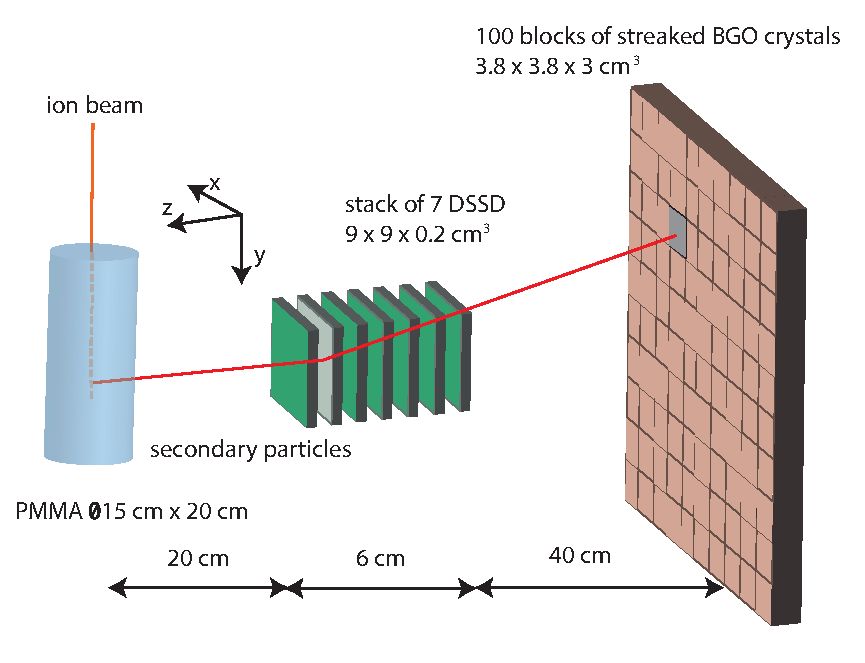
\includegraphics[width=0.7\textwidth]{03_GraphicFiles/chapter3/HT/Compton_Camera_hadontherapy_PMMA_Cylinder_EN.pdf}
  \caption{Scheme of the simulation setup (not at scale): a PMMA cylindrical phantom is set in front of the Compton camera prototype. The Compton camera is composed of a stack of 7 double sided silicon strip detectors (scatterer) and a plan of 100 single BGO blocks. The set distances are realistic for clinical conditions. This geometrical configuration has been used for all the simulations presented in this work.}
  \label{fig:fig_setup_CC_simulation_Hadronth}
\end{figure}

The silicon detectors have a strip pitch of 1.4~mm, for a total of 64 strips per side (double-sided readout based on electron and hole pairs collection). 
Regarding the BGO blocks, their entrance surface is streaked in a 8$\times$8 matrix of pseudo-pixels, $4.4\times4.4$~mm$^{2}$ size, and the readout is performed via 4 photo-multiplier tubes. The position reconstruction is achieved via Anger logic.

A scheme of the simulation setup is given in figure~\ref{fig:fig_setup_CC_simulation_Hadronth}. The ion beam interacts with a cylindrical PMMA (PolyMethylMethAcrylate) phantom (15~cm diameter and 20~cm length) placed in front of the Compton camera as target. It is placed 20~cm far from the first silicon plane (center-to-center distance) which seems a realistic distance in clinical conditions. The distance between the last silicon layer and the absorber array (center-to-center) is set to 40~cm in order to permit time-of-flight measurements (see section~\ref{MatMeth::TOF_Ecut}).

The silicon detector strips are not reproduced in the simulation code, and the transverse spatial resolution is set to 0.9~mm FWHM at the reference energy of 1~MeV, according to preliminary measurements performed on smaller detector prototypes. Concerning the transverse direction (perpendicular to the beam line), the interaction position is set to the center of the involved silicon plane. A mono-block crystal is simulated for the absorber for simplicity. The events are selected to be limited to a single block component based on the interaction localization, and the interaction position is reconstructed via center of gravity calculation if multiple interactions occur. An uncertainty contribution, randomly extracted by a Gaussian of 5~mm FWHM, is added to the reconstructed position to mimic the pseudo-pixel-based readout. For what concerns the parallel direction, given the fact that the employed BGO blocks have not depth of interaction reconstruction capabilities, the interaction position is fixed to the center of the mono-block crystal.

The energy resolution of the BGO blocks was estimated in preliminary measurements and is accordingly set to 17\% FWHM at the reference energy of 667~keV (a 137-cesium source has been used for the measurements). The energy resolution of the silicon detector is set to 5~keV (FWHM) according to the design expectations.

The time resolution has been set to 3.0~ns FWHM for the BGO blocks and to 15.0~ns FWHM for the silicon slabs, according to preliminary measurements performed on test detector modules at the GANIL %(Grand Accelerateur National d'Ions Lourds) 
center in France.

The detector resolutions play an important role in the Compton camera performances. The spatial resolution of the absorber influences the position of the apex of the Compton cone as well as its axis orientation. The energy resolution of the scatterer determines the Compton cone aperture angle. The time resolution impacts the coincidence window between the absorber and the scatterer, and therefore the detectors ability to distinguish between true and random coincidences.

The CLaRyS project also includes the development of a beam tagging hodoscope, composed of scintillating fibers read out by multi-channel photomultipliers. This detector is used to synchronize the beam time and space structure to the prompt gamma detection in order to tune the detection window reducing the background contamination. In addition to this, the spatial localization of the impinging beam bunch can be included in the event reconstruction algorithm to add constraints to the obtained solutions (see section~\ref{MatMeth:reconstruction}). The hodoscope is not included in the simulation, but its spatial and time resolution have to be taken into account for the time-of-flight discrimination (see section~\ref{MatMeth::TOF_Ecut}) and events reconstruction. They are set to 1~ns and 1~mm FWHM, respectively.\\ 
The detector's spatial, energy, and time resolutions are summarized in table \ref{table:table_resolution_detecteurs_CC_simulation_Hadronth}.

\begin{table}
\centering
%\begin{tabular}{>{\columncolor[gray]{0.9}}ccc}
\caption{Estimations of reachable resolutions with the detectors. Those resolutions are applied during the simulations.}
\begin{tabular}{cccc}
\hline
\textbf{Resolution (FWHM) at 1~MeV} & \textbf{Scatterer} & \textbf{Absorber} & \textbf{Hodoscope}\\
\hline 
\textbf{spatial [mm]	}			 &     0.9		 &  5 &	 1\\
%\hline
\textbf{energy}				&	5~keV		&  17~\%	&	/\\
%\hline
\textbf{timing [ns]}	        		&	15			&	3 	&  1\\
\hline
\end{tabular}
\label{table:table_resolution_detecteurs_CC_simulation_Hadronth}
\end{table}
    
The Monte Carlo simulation is performed with the Geant4 toolkit, version 9.6.02. 
%Geant4 has been developed at CERN %(Conseil europ\'{e}en pour la recherche nucl\'{e}aire) for high energy physics experiments, but it has been shown that it can be used for ion beam therapy studies \cite{cirrone_hadrontherapy_2011,toshito_new_2010}. 
%Some improvements are still needed in order to extend the hadronic models to low energy applications~\cite{dedes_assessment_2014, Pinto:2016aa}.
The particle interactions in matter are described in this work by means of the models listed in table~\ref{table:table_modele_physic_CC_simulation_Hadronth}. Additionally, the Doppler broadening and the photon polarization effects are included.
 

\definecolor{Gray}{gray}{0.9}

\begin{table}
\label{physlist_ion}
\caption{Hadronic models used in the Geant4 simulations.}
\begin{scriptsize}
\begin{center}
\renewcommand{\arraystretch}{1.2}
%\begin{tabular} {>{\columncolor[gray]{0.9}}cccc}\hline  
\begin{tabular} {cccc}\hline
%\rowcolor{Gray}
\textbf{Process} & \textbf{Protons} & \textbf{Ions} & \textbf{Neutrons} \\ \hline 
\textbf{Electromagnetic} & \multicolumn{3}{c}{standard$_{\rm{option3}}$} \\ %\hline
\textbf{Inelastic} & G4BinaryCascade & G4QMDReaction  &  G4BinaryCascade  \\ 
 & & (G4IonsShenCrossSection)&+ G4NeutronHPInelastic ($<$19~MeV)\\ %\hline
\textbf{Elastic} & G4LElastic & G4LElastic & G4LElastic + G4NeutronHPElastic ($<$19~MeV)\\ %\hline
\textbf{Fission} & / & / & G4LFission + G4NeutronHPFission($<$19~MeV) \\ %\hline
\textbf{Capture} & / & / & G4LCapture +  G4NeutronHPCapture ($<$19~MeV) \\ %\hline
\textbf{Radioactivedecay} & / & G4Radioactivedecay & / \\ \hline
\end{tabular}
\end{center}
\end{scriptsize}
\label{table:table_modele_physic_CC_simulation_Hadronth}
\end{table}

%\subsection{Data processing}
%\label{subsection:Treatment_data_CC_hadrontherapy_Geant4}

\subsection{Beam structure}
\label{subsection:modelisation_fasceau_ions_CC_hadrontherapy_Geant4}
\subsubsection{Beam structure measurements at HIT}\label{beam_measurement}
Our group performed a set of measurement to characterize the beam time structure of the synchrotron installed in the Heidelberg Ion Therapy Center (HIT), Germany~\cite{HIT_timestructure}. This set of measurements extends the results reported in~\cite{HIT_timestructure} and is then used to reproduce a realistic beam in the simulation.\\
The beam characterization has been performed for 200~MeV/u and 400~MeV/u primary ion energy with a two-fiber hodoscope (basic prototype of the one at present under development) and the spill signal was given by the accelerator. Figure \ref{fig:fig_structure_temps_faisceau_HIT_2013_CC_simulation_Hadronth} shows the results for carbon ions at 400~MeV/u. The pulses have a spill period of 150.2~ns and each bunch is approximately 21.5~ns.
The mentioned measurements have shown that the spill phase changes during the extraction: this implies that the HF signal from the synchrotron can not be used to trigger the pulses, so that the use of an additional beam time stamp system like the hodoscope seems required for time-of-flight background rejection purposes.

\begin{figure} [!hbtp]	
  \centering
  %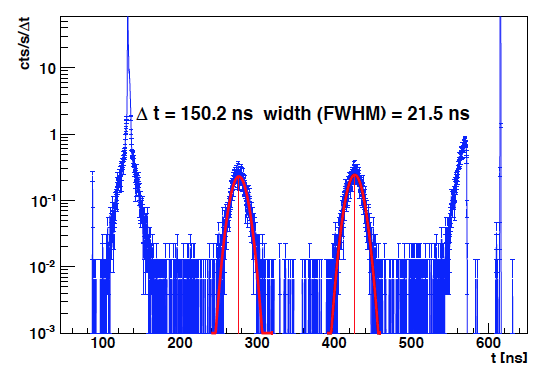
\includegraphics[width=0.6\textwidth]{./Figure/2013_Structure_Time_Beam_400MeV.png}
  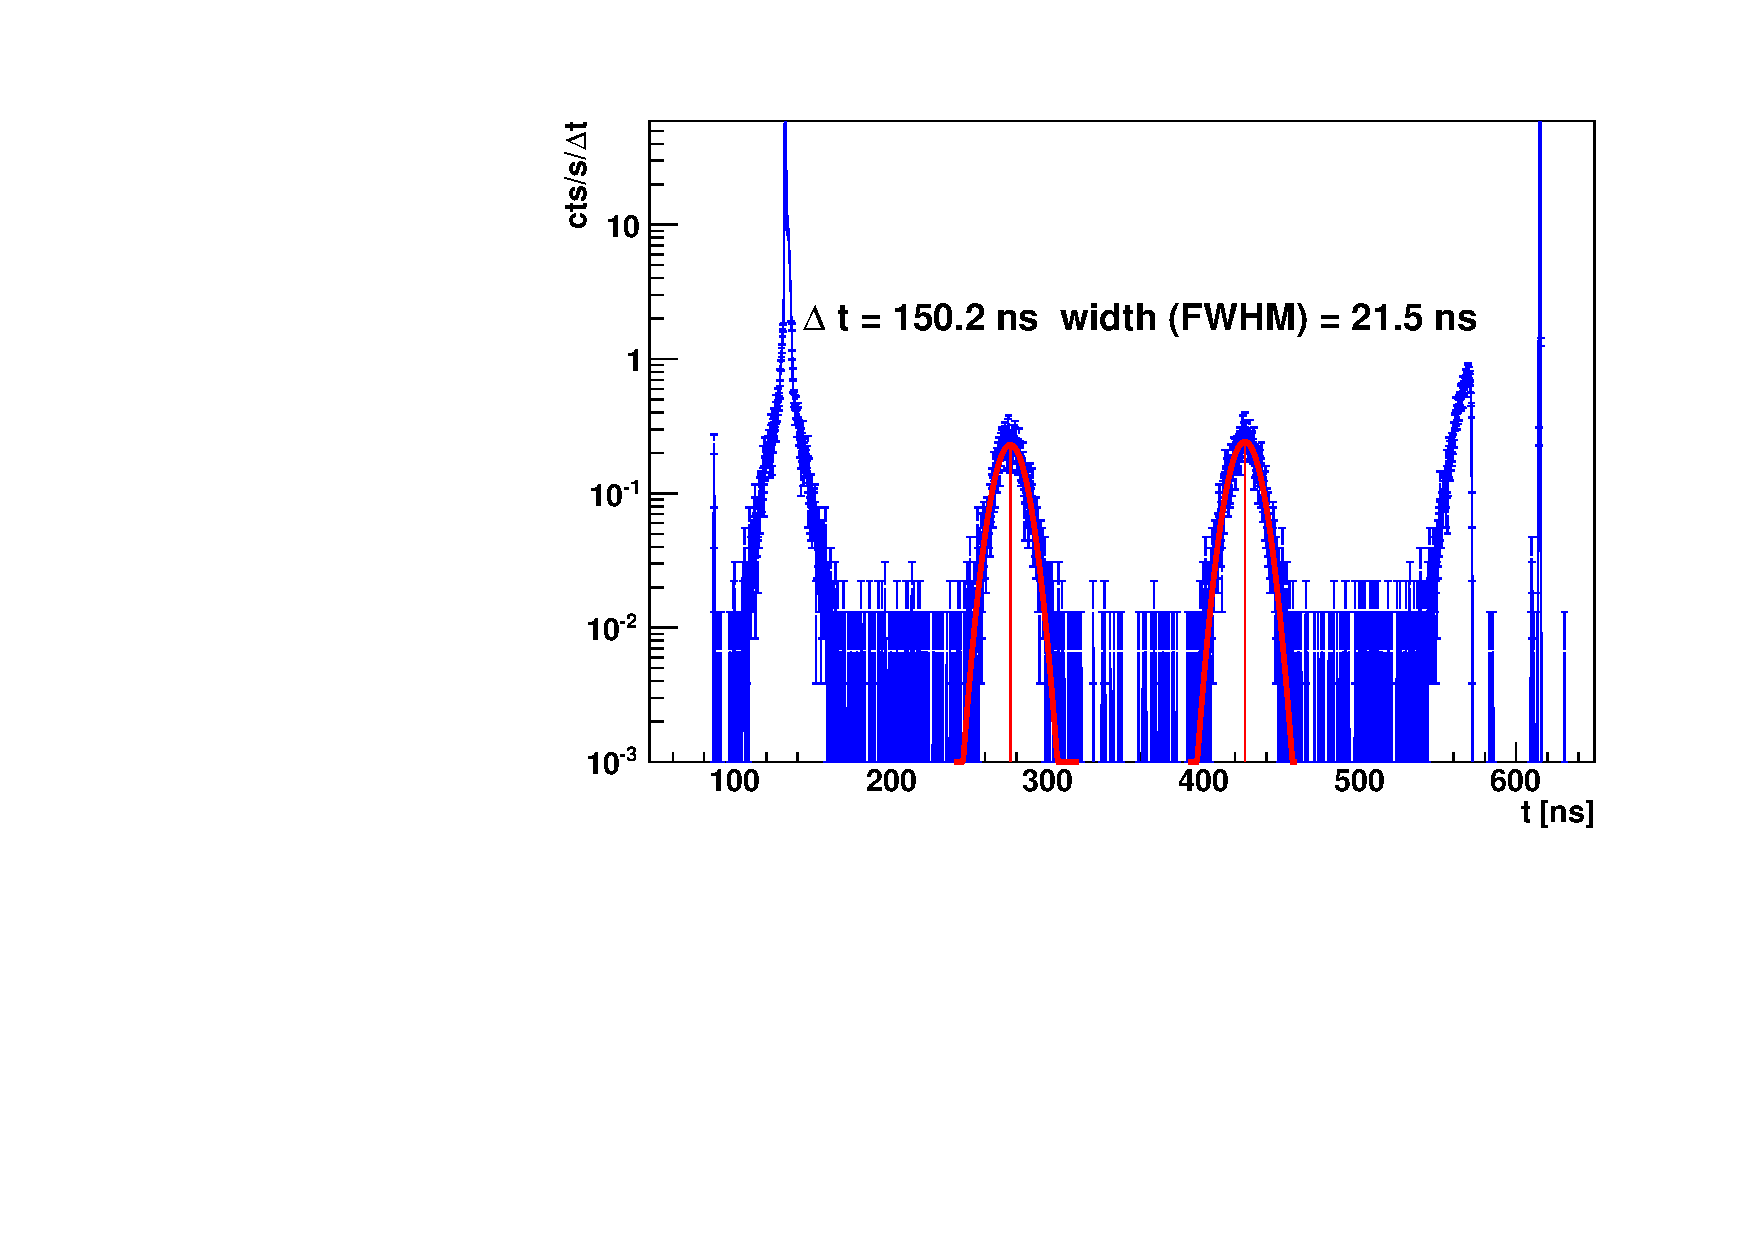
\includegraphics[width=0.6\textwidth]{03_GraphicFiles/chapter3/HT/fiber_vert_hor_run14.pdf}
  \caption{Time micro-structure measured from a carbon ion beam at 400~MeV/u delivered at HIT. The pulses have an extraction period of 150.2~ns and the bunches are 21.5~ns FWHM.  On the x axis the time has been measured with a two-scintillating-fiber hodoscope, with 1~ns FWHM time resolution.}
  \label{fig:fig_structure_temps_faisceau_HIT_2013_CC_simulation_Hadronth}
\end{figure}


\subsubsection{Beam modeling}\label{beam_modeling}
The two main beam particles used in clinics are considered in the simulation: protons and carbon ions. The beam range of interest is 15.2~cm in the PMMA phantom, and the associated energy is 160~MeV for protons and 305~MeV/u for carbon ions.\\ 
The beam transverse dimension is modeled with a Gaussian distribution with a standard deviation of 5~mm for protons at 160~MeV and 3.5~mm for carbon ions at 305~MeV/u. The number of incident ions for a spot in pencil beam scanning (PBS) mode is $10^8$ for protons (distal spot - upper intensity limit) and $10^5$ for carbon ions (average spot intensity)~\cite{Kramer:2000aa, Grevillot_2011,smeets_2012}. In the simulation, the beam intensity is modeled by an average number of particles per bunch. The exact number of particles in each bunch is given by a random extraction from a Poisson distribution, where the mean value is the selected beam intensity.\\
The beam time structure is applied at the data analysis stage. Two different time structures have been considered for this study, related to two kinds of accelerators used in clinical practice: the IBA C230 cyclotron for protons (used in 16 clinical centers worldwide) and the HIT synchrotron for carbon ions. For protons at 160 MeV, the primary particles are grouped in bunches of 2~ns (this value may vary also according to the distance between the cyclotron and the treatment room, and energy spread selection) at a frequency of 106~MHz (9.42~ns)~\cite{Roellinghoff_2014}. The clinical beam intensity is 3.2~nA which corresponds to about 200 protons per bunch. Concerning the carbon ion beam at 305~MeV/u, the simulated time structure refers to the measurements presented in section~\ref{beam_measurement}. We used 30~ns duration bunches a frequency of 5.9~MHz (170~ns period). The clinical beam intensity for carbon ions is $5\times10^7$~ions/s during extraction, corresponding to about 9~ions per bunch. 

The coincidence window (between scatterer and absorber events) is set to 40~ns, centered on each absorber detected interaction. This value is adapted to the detectors time resolutions. At the simulation stage, each interaction in the detector layers is collected with the related local time. The beam time structure is then applied to each single hit, and the selected coincidence window is used to retrieve scatterer-absorber coincidence events.\\ 
Table~\ref{table:definition_beam_structure_CC_hadrontherapy_Geant4} summarizes the presented beam time structures and coincidence reconstruction features.

\begin{table} [!htbp]
\footnotesize
\centering
\caption{Description of the two beam structures studied: the IBA cyclotron C230 for protons and the synchrotron installed at the Heidelberg Ion Therapy Center (HIT) in Germany for carbon ions. The macro-structure of the synchrotron, at the second time scale, is not considered here. The beam structures are applied to the simulation data.}
\setlength{\tabcolsep}{2pt}
%\hspace{-2.1cm}
\begin{tabular}{c|c|cc}
%\cline{2-4}
\hline
		\multicolumn{2}{c}{ }		 & 					\textbf{Protons} & \textbf{Carbon ions}\\ 
\hline
%\cline{2-4}%\hline
\multirow{3}{*}\textbf{Clinical features}		&	Facility	& IBA Cyclotron C230 &   Synchrotron at HIT\\
											& Clinical intensity& $  2\times10^{10}$ p/s  & $  5\times10^{7}$ ions/s\\
											& Energy 			&160~MeV 			&    305~MeV/u\\
%\cline{2-4}%
\hline
\multirow{3}{*}\textbf{Beam structure}		&	Bunch time [ns]	& 3.2				&  30\\
											& Period [ns]		&   9.4 				& 170\\
											& Primaries/bunch 	&217 			& 9\\
%\cline{2-4}%
\hline
\multirow{2}{*}\textbf{Detectors}						& Coincidence window [ns]		& 40 	&  40 \\
											&Time resolution (FWHM) [ns] & \multicolumn{2}{c}{Si: 15 and BGO: 3}\\
%\cline{2-4}%
\hline
\end{tabular}
\label{table:definition_beam_structure_CC_hadrontherapy_Geant4}
\end{table}



%\newpage
%---------------------------------------------------------------
%---------------------------------------------------------------
\subsection{TOF and energy based data selection}
\label{MatMeth::TOF_Ecut}

The Compton detection principle is based on a double interaction in the scatterer and absorber section, where an interaction is defined as an energy deposit in a detector module. As discussed in section~\ref{subsection:modelisation_fasceau_ions_CC_hadrontherapy_Geant4}, the coincidence reconstruction relies on a defined time window, fixed according to the detector resolution. In a simulation environment, different kinds of coincidence events can be distinguished and studied: 
\begin{itemize}
\item[-] real coincidences: created by a single photon first interacting in a single scatterer plane and then in a single absorber block;
\item[-] quasi-simultaneous interaction of two secondary particles;
\item[-] double interaction of the same particle, not a photon (e.g. protons, neutrons).
\end{itemize}

In an experiment the collected data are affected by a certain number of the so-called random coincidences, which cannot be experimentally distinguished from true coincidences, from the timing coincidence point of view. The amount of random coincidences depends on the detector time resolutions, the fixed time coincidence window and the beam time structure, the phantom composition and camera prototype setup. In figure~\ref{fig:fig_explication_coincidence_CC_simulation_Hadronth}, a schematic view of the different kinds of coincidences is presented.

\begin{figure}
  \centering
  \includegraphics[width=0.9\textwidth]{03_GraphicFiles/chapter3/HT/Schema_coincidence_EN.eps}
  \caption{Diagram showing the different definitions of coincidences in the Compton camera.}
  \label{fig:fig_explication_coincidence_CC_simulation_Hadronth}
\end{figure}

In addition to this, the prompt gamma measurement is contaminated by other secondary particles (mainly massive and charged particles like protons and neutrons), produced by the interaction of the primary particles with the patient/phantom.
Ad-hoc filtering methods are applied to reduce the above described contamination.

\begin{itemize}
\item Time-Of-Flight: it has been demonstrated that a time-of-flight discrimination is possible and effective in reducing the background generated by massive particles interactions~\cite{Testa:2010aa}. The massive particles approach the detector at a lower speed with respect to photons. The time information provided by the hodoscope and the absorber can be combined to fix a detection time window and reject all the events outside the window. The time elapsed between the incident particle creation ($\mathrm{t_{creation}}$) and the secondary particle detection in the absorber ($\mathrm{t_{absorber}}$) is considered as the time-of-flight. The particle creation time is modeled according to the beam time structure, as presented in section~\ref{beam_modeling}. The detection time in the absorber is calculated with the simulation local time of the hit in the detector layer. The hodoscope time resolution (1~ns FWHM) is applied to the primary particle creation time, with a contribution randomly extracted from a Gaussian with $\sigma\,=$ 1/2.35~ns ($u_{\mathrm{hodoscope}}$) . The detection time in the absorber is affected by the absorber time resolution, already included in the simulation code.

 \begin{eqnarray}
%TOF = t_{\mathrm{absorber}}-t_{\mathrm{hodoscope}} \\
TOF_{\mathrm{simulation}} = t_{\mathrm{absorber}}-(t_{\mathrm{creation}} + u_{\mathrm{hodoscope}})
\label{TOF_equation}
\end{eqnarray} 

The time-of-flight spectrum resulting from the simulation shows that the coincidences of interest (produced by prompt-gamma rays) are included in a window between 0 and 8~ns (figure \ref{fig:fig_TOF_distribution_CC_simulation_Hadronth}). Therefore, all the coincidences with a TOF no included in this time window have been rejected.
\begin{figure}	
  \centering
  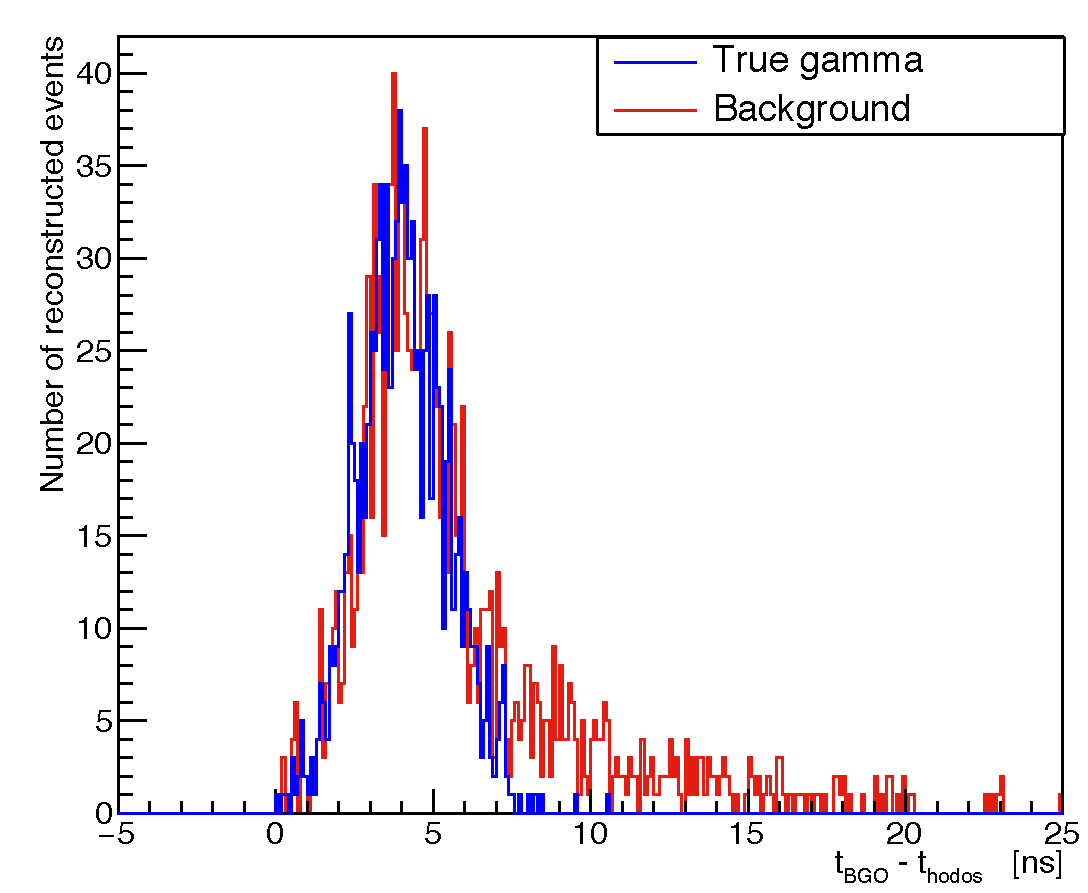
\includegraphics[width=0.6\textwidth]{03_GraphicFiles/chapter3/HT/TOFspectra_2}
  \caption{Time of flight spectra of true gamma coincidences (blue) and background events (red) obtained with $10^{8}$ 160~MeV incident protons.}	
  \label{fig:fig_TOF_distribution_CC_simulation_Hadronth}
\end{figure}

\item Energy selection: energy thresholds are defined for the event detection. 50~keV and 100~keV are set as lower threshold for the energy deposited in a single silicon layer and absorber, respectively. For a complete event, a total absorbed energy lower limit is set to 1~MeV. In addition to the effect of background rejection, this selection also reduces the impact of partially absorbed photons and events with Compton electron escape.

Further energy selections, assuming for instance $E_1+E_2$ equal to one of the strong gamma lines, have been applied by other authors. Also, filters checking the possibility of reconstructing a Compton cone could be used. At this stage we did not consider such approaches, in order to cope with simple considerations on signal to noise on raw data.

\end{itemize}

\subsection{Reconstruction algorithms}
\label{MatMeth:reconstruction}
Once the coincidences are defined and selected according to the fixed physical cuts, the prompt-gamma emission point has to be reconstructed for each event. This can be done via analytic or iterative algorithms based on the Compton kinematics. Both are presented in the following sections.


\subsubsection{Line-cone algorithm}
The reconstruction via line-cone algorithm exploits the energy deposit and position information collected by the camera in addition to the beam spatial information provided by the hodoscope. Thanks to the deposited energies in the detectors and the interaction positions, a cone surface is analytically defined via the Compton equation~\ref{Compton_equation}. Figure~\ref{fig:reconstruction_scheme} shows a sketch of the reconstruction principle. The interaction position in the scatter gives the cone apex and the line connecting the interaction positions in scatterer and absorber gives the cone axis. We assume that the initial energy of the gamma ray is fully absorbed in the absorber. According to previous simulation results, the rate of events fully absorbed in the Compton camera is more than 60~\% in the PG energy range. In order to constrain the reconstruction, the beam direction is used to limit the possible solutions (lying on the reconstructed cone surface) to two points (intersection of the beam direction and the reconstructed cone). The set of all the reconstructed points gives the emission source distribution. The final image is the mono-dimensional projection of the prompt gamma emission spectrum. 

\begin{figure}
\centering
  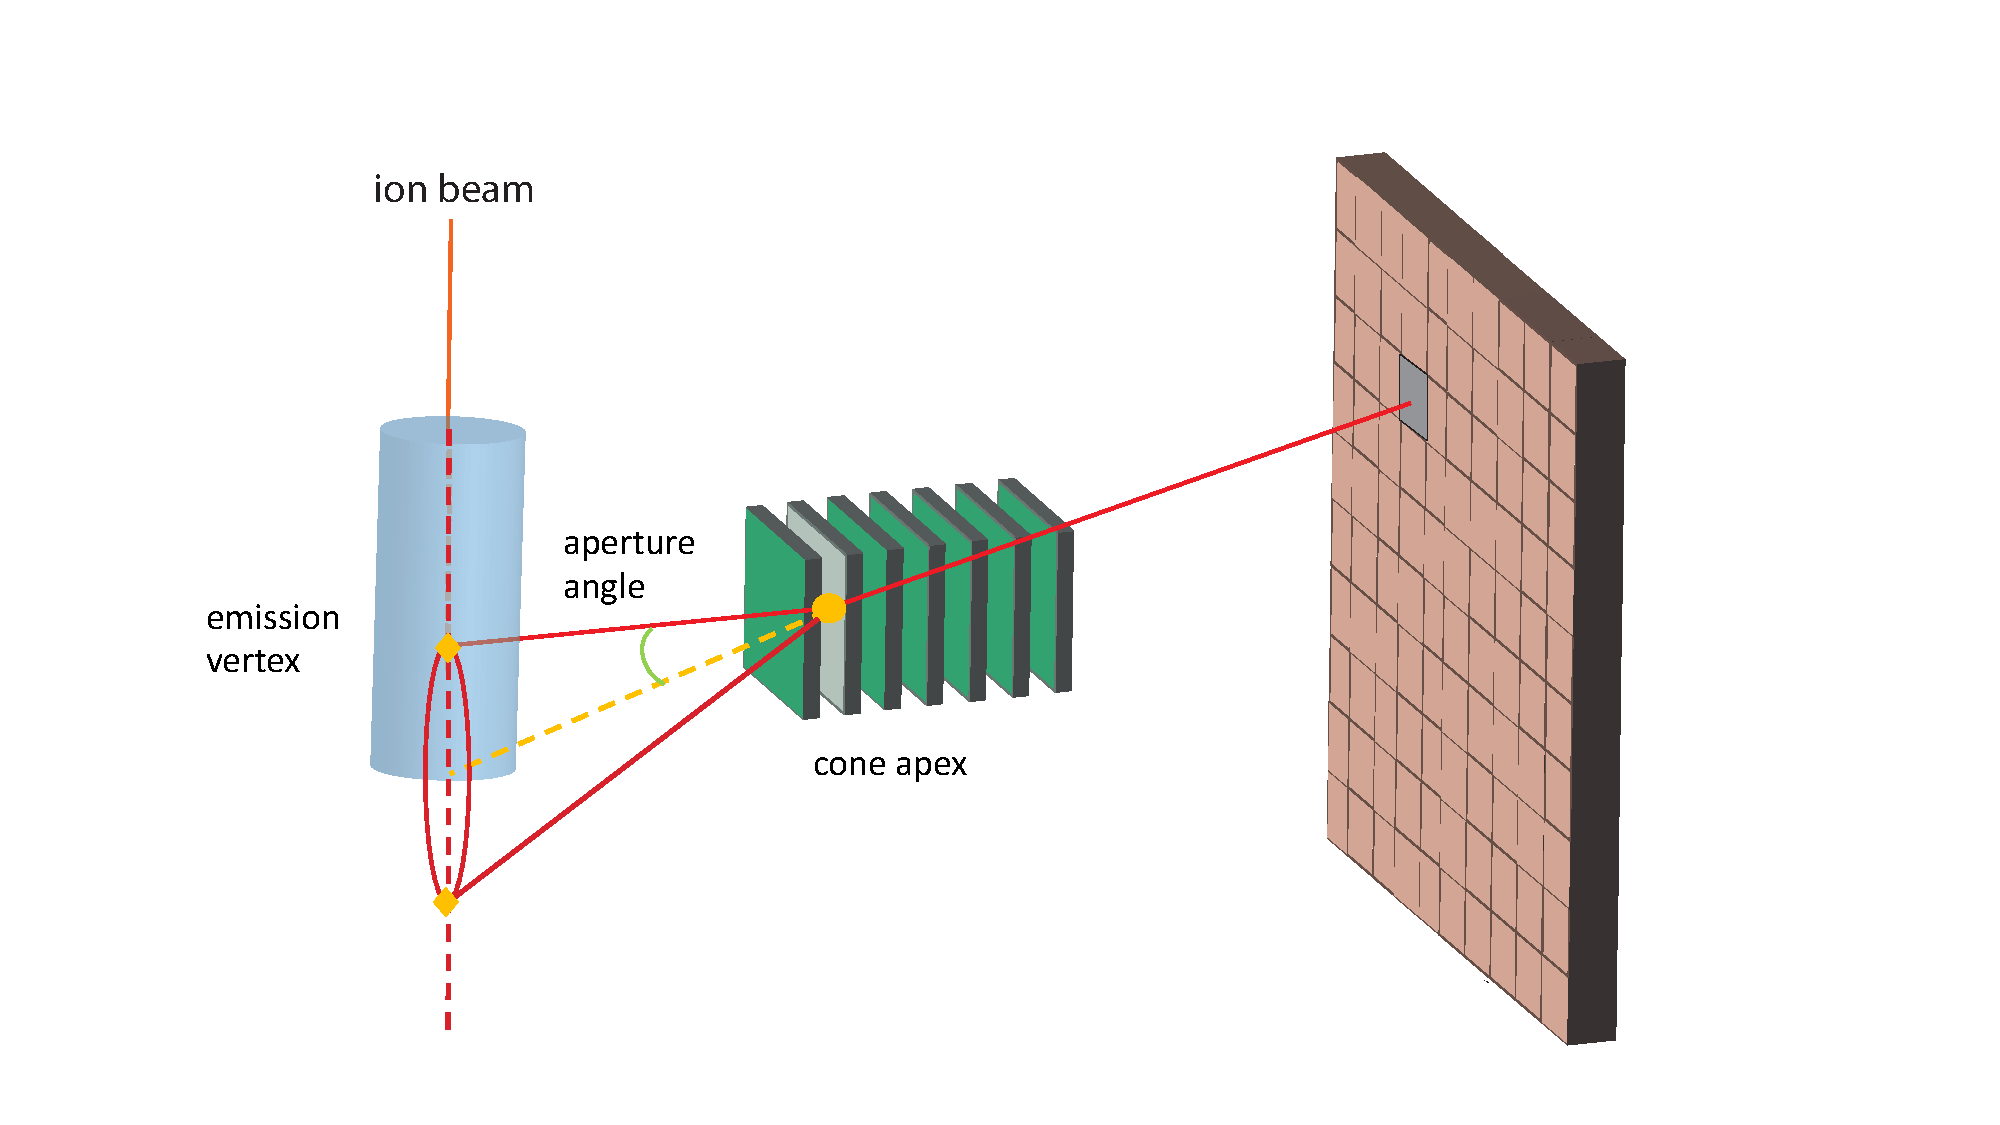
\includegraphics[width=0.8\textwidth]{03_GraphicFiles/chapter3/HT/reconstruction_scheme}
  \caption{Scheme of the reconstruction principle for Compton events. For line-cone reconstruction methods, two points are extracted for each event (diamonds in the figure), provided by the intersection between the reconstructed Compton cone and the beam line. The reconstructed image is strictly 1D. For the iterative MLEM algorithm, each algorithm iteration adds constraints to the reconstructed cone surfaces, leading to  a 3D image.}	
  \label{fig:reconstruction_scheme}
\end{figure}

\subsubsection{LM-MLEM algorithm}	
The iterative methods allow to get a 3D image reconstruction, potentially by taking into account the spatial resolution and the energy resolution of the detectors. Few iterative algorithms have been developed for Compton event reconstruction~\cite{schone_common_2010, zoglauer_design_2011,gillam_compton_2011,mackin_evaluation_2012,lojacono_low_2013}.

The \textit{List-Mode Maximum Likelihood Expectation Maximization} (LM-MLEM) algorithm is an MLEM version which allows to reconstruct the image directly from the list of detected events.
The LM-MLEM algorithm used for this study is detailed in~\cite{hilaire_compton_2014}.%\cite{maxim_filtered_2014,hilaire_compton_2014}.%\cite{maxim_analytical_2009,lojacono_low_2013,maxim_filtered_2014,hilaire_compton_2014}.\newline

%The first step is to define the volume which includes the origin of the prompt gamma ray detected. This volume is divided into equal voxels and the emission intensity is assumed homogeneous for each voxel $j$, with a Poisson distribution of parameter $\lambda_j$ (a vector of the emissions intensities of all the voxels). The algorithm is based on a system matrix $T$ composed of the coefficients  $t_{ij}$ which represent the probability that a photon produced in the voxel $j$ is detected in coincidence by the Compton camera as an event $i$. The probability for a gamma detected in coincidence to be emitted from the voxel $j$ is denoted as $s_j$.
%The LM-MLEM algorithm starts with an initial value $\lambda^{(0)}_j$, which can be the simple back-projection reconstruction.
%The iterations rely on the following recurrence relation:
%
%\begin{equation}
%\lambda_j^{(l+1)} =  \frac{\lambda_j^{(l)} }{s_j} \sum\limits_{i=1}^{N_{\gamma}} t_{ij} \frac{1}{P_i^{(l)}},\quad \rm{with}\quad  P_i^{(l)}=\sum\limits_{k=1}^{N_{v}} t_{ij}\lambda_k^{(l)},
% \label{eq:equation_lambda_compton_med_nucleaire}
%\end{equation}
%where $N_{\gamma}$ is the number of detected events and $N_v$ is the number of voxels in the image.
%
%For each photon detected, the coefficients in column i are calculated by taking into account the uncertainties on the angle between the source and the involved scatterer plane and the angle between the scatterer plane and the absorber involved module.
%The matrix elements $t_{ij}$ are calculated as:
%\begin{equation}
% t_{ij} = K(\beta_i,E_{tot})\frac{|\rm{cos}(\theta_{{V_2V_1}}) |}{V_2V_1^2} \int\limits_{M\in v_j} \frac{|\rm{cos}(\theta_{V_1M})|}{V_1M^2} h_i(M)dv,
% \label{eq:equation_tij_compton_med_nucleaire}
%\end{equation}
%where $\beta_i$ is the Compton scattering angle, $V_1$ the interaction position in the scatterer, $V_2$ the interaction position in the absorber, $h_i$ the spatial kernel which models the uncertainties on the Compton angle for each voxel $M$, $K(\beta_i,E_{tot})$ the differential cross section and $v_j$ the reconstructed volume.
%
%In order to simplify and speed up the calculation of the $t_{ij}$ matrix, the voxels located far from the reconstructed cone are set to 0. The distance between the cone and the voxel is calculated by taking the voxel center as reference point. %The spatial resolutions are not included in this version of the algorithm.\newline
%For each iteration, the matrix $T$ is stored and the reconstructed image can be produced.


\subsection{Performance study}
\label{MatMeth:performance}
In this section the parameters studied for the camera performance evaluation are explained. The study is mainly divided into three sections:
\begin{itemize}

\item Absolute efficiency: the camera absolute efficiency for gamma detection is studied by means of mono-energetic irradiation with point-like sources;
\item Rate of random coincidences: with proton and carbon beams interacting with the PMMA phantom, the rate of random and true detected coincidences is studied as a function of the beam intensity;
\item Camera precision: the camera capability of identifying the fall-off of the prompt-gamma emission profile is tested and the two reconstruction methods presented above are compared. 

\end{itemize}


\subsubsection{Absolute detection efficiency}
The absolute efficiency is crucial for the Compton camera performances and for its possible application in treatment monitoring. An efficient monitoring system should be ideally in real time, in order to allow for a treatment adaptation or interruption in case of severe issues detected in the delivered dose profile with respect to the planned treatment. In order to achieve an online detection of such deviations, given the limited prompt gamma emission rate per incident ion~\cite{Ortega:2015aa}, a high detection efficiency is required to perform a monitoring on, ideally, a beam spot basis. In addition to this, the absolute detection efficiency directly affects the image reconstruction quality, which is in general increased for increased statistics.

In order to well define the expected camera efficiency, it has been studied with the irradiation from point-like mono-energetic gamma sources, set in different positions with respect to the center of the camera on the transverse plane.	

The absolute efficiency $\epsilon$ is defined as:
\begin{equation}
\epsilon =\frac{\mathrm{N}\gamma_{\mathrm{coinc}}}{\mathrm{N}\gamma_{\mathrm{total}}},
\end{equation}
\label{eq:equation_efficacite_absolue}
with $N\gamma_{\mathrm{coinc}}$ the number of gamma events corresponding to true coincidences, $N\gamma_{\mathrm{total}}$ the total number of emitted gammas.

The setup is the same as figure~\ref{fig:fig_setup_CC_simulation_Hadronth}, with the exception of the PMMA phantom which is removed to leave the gamma source in air.
The point-like source is set in the range $-300$~mm to $+300$~mm (with the center of the camera transverse section set in the position 0), and moved in variable length steps: 20~mm close to the center of the camera, then increasing up to 1~cm for the most peripheral point. The movement followed the transverse axis of the camera. Different energies have been tested to mimic different prompt gamma lines: 300~keV, 500~keV, 1~MeV, 2~MeV, 4~MeV, 6~MeV. No time structure is reproduced for this part for the study.\\
Moreover, the rate of events with a almost full primary energy absorption has been studied as a function of the primary gamma energy and the position in the range presented above. The threshold for the energy absorption has been set to 90\% of the primary gamma energy.\\ 

\subsubsection{Rate of random coincidences}

As the Compton detection principle relies on time coincidences, in addition to the main importance played by the detectors energy resolutions, the beam intensity and time structure are important parameters to be studied in order to assess the possible clinical implementation of a Compton detection based monitoring of ion beam treatment. The ability of the detection system to distinguish between true and random coincidences, i.e.~the resulting signal over noise ratio, strongly depends on the beam time structure. The number of true and random coincidences (where the two cases listed in section~\ref{MatMeth::TOF_Ecut} are included in the random coincidences) is studied as a function of the beam intensity, before and after data reconstruction via line-cone algorithm~(see section~\ref{MatMeth:reconstruction}).

The range of intensities is defined in order to cover a wide range of operation: from a very low beam intensity to a realistic clinical particle rate. Therefore, for proton and carbon ions, the lowest beam intensity is set to 0.1 particles per bunch on average, while the upper limit is set to 217 protons or 70 carbon ions per bunch. All the simulations are performed with a total of $10^{8}$ primary protons and  $2\times10^{5}$ primary carbon ions (see section~\ref{beam_modeling}). For the analysis of the results, the coincidence yields are scaled to the number of incident ions and the beam intensity to the average number of ions per bunch.

\subsubsection{Camera precision}
\label{MatMeth:precision}

The camera precision is defined as the difference between the predicted PG fall-off position - FOP - (according to the treatment planning) and the detected one.
In this study, a reference profile has been defined as the reconstructed emission vertex profile at high statistics ($\mathrm{10^{10}}$ incident protons). This Bragg peak position is used as reference and compared to the ones at lower statistics, deduced as described in the following.

For the LM-MLEM reconstruction, the reconstruction volume is set to $20\times40\times1$~cm$^3$ around the expected FOP, with a $100\times200\times5$ voxel matrix. To be noticed that the two reconstruction methods produce different results: the line-cone method is based on the beam direction information, so that it naturally returns a mono-dimensional image as result, while the LM-MLEM method is able to reconstruct the prompt-gamma emission distribution in three dimensions. A mono-dimensional projection along the beam direction is used for the falloff identification and for a direct comparison of the line-cone method.
The \textit{SmoothKern} method, with the Nadaraya-Watson regression~\cite{Nadaraya_regression, Watson_regression}, is used to smooth the reference profiles in order to reduce relative statistical fluctuations.

A region of interest (ROI) ranging from $y=0$ mm to $y=+100$ mm is defined around the expected Bragg peak position, located at $y=+50$~mm in the phantom. The reference reconstructed profiles are modeled in the ROI by a linear combination of Non-Uniform Rational Basis Splines (NURBS)~\cite{NURBS}. 

The reference data set is normalized in order to obtain lower statistics profiles, in the range 1$\times$10$^8$ to 5$\times$10$^9$. Statistical fluctuations, randomly extracted following a Poisson law, are added to the obtained PG profiles to mimic realistic reconstructed profiles. This method is used to reduce the analysis time.

For each chosen statistics, 1000 PG profiles are generated and a custom minimization method is applied to deduce the minimal shift between the reference profile and the one at lower statistics. The minimization algorithm shifts the reference profile in a 60~mm range, between $-30$~mm and $+30$~mm with respect to the initial position, with a step of $0.1$~mm, and for each position it compares its position to the low statistics profile by calculating the $\chi^2$ as follows:
\begin{eqnarray}
\chi^2 = \sum\limits_{i=1}^{N_{bin}} {(y_{\mathrm{sample,i}}-y_{\mathrm{NURBS,i}})^2},
\end{eqnarray}
where for every bin $i$ $y_{\mathrm{sample}}$ is the number of events in the low statistics profile, $y_{\mathrm{NURBS}}$ is the number of events for the reference profile NURBS (scaled at the same low statistic). Several minimization algorithms are available, but in order to avoid artifacts at low statistic, a robust custom defined approach has been preferred.

%Figures~\ref{fig:fig_Results_Chi2_Distribution_Variation_CC_simulation_Hadronth_LC} and~\ref{fig:fig_Results_Chi2_Distribution_Variation_CC_simulation_Hadronth_MLEM} show the distribution of $\chi^2$ calculated for a low statistic profile at $10^8$ incident protons.

The global minimum of all the calculated $\chi^2$ is then retrieved and the shift associated to this value is added to the shift distributions. % shown in figure~\ref{fig:fig_Results_Precision_Distribution_Variation_CC_simulation_Hadronth_LC} and~\ref{fig:fig_Results_Precision_Distribution_Variation_CC_simulation_Hadronth_MLEM} for the line-cone and LM-MLEM algorithm respectively, for $10^8$ incident protons. 
The standard deviation of the distribution resulting of the thousand results gives the precision of the camera for a given number of incident protons. 



% \begin{figure}
% \centering
% \subfloat[\label{fig:fig_Results_Estimation_Camera_Profil_highStat_CC_simulation_Hadronth_LineCone}]{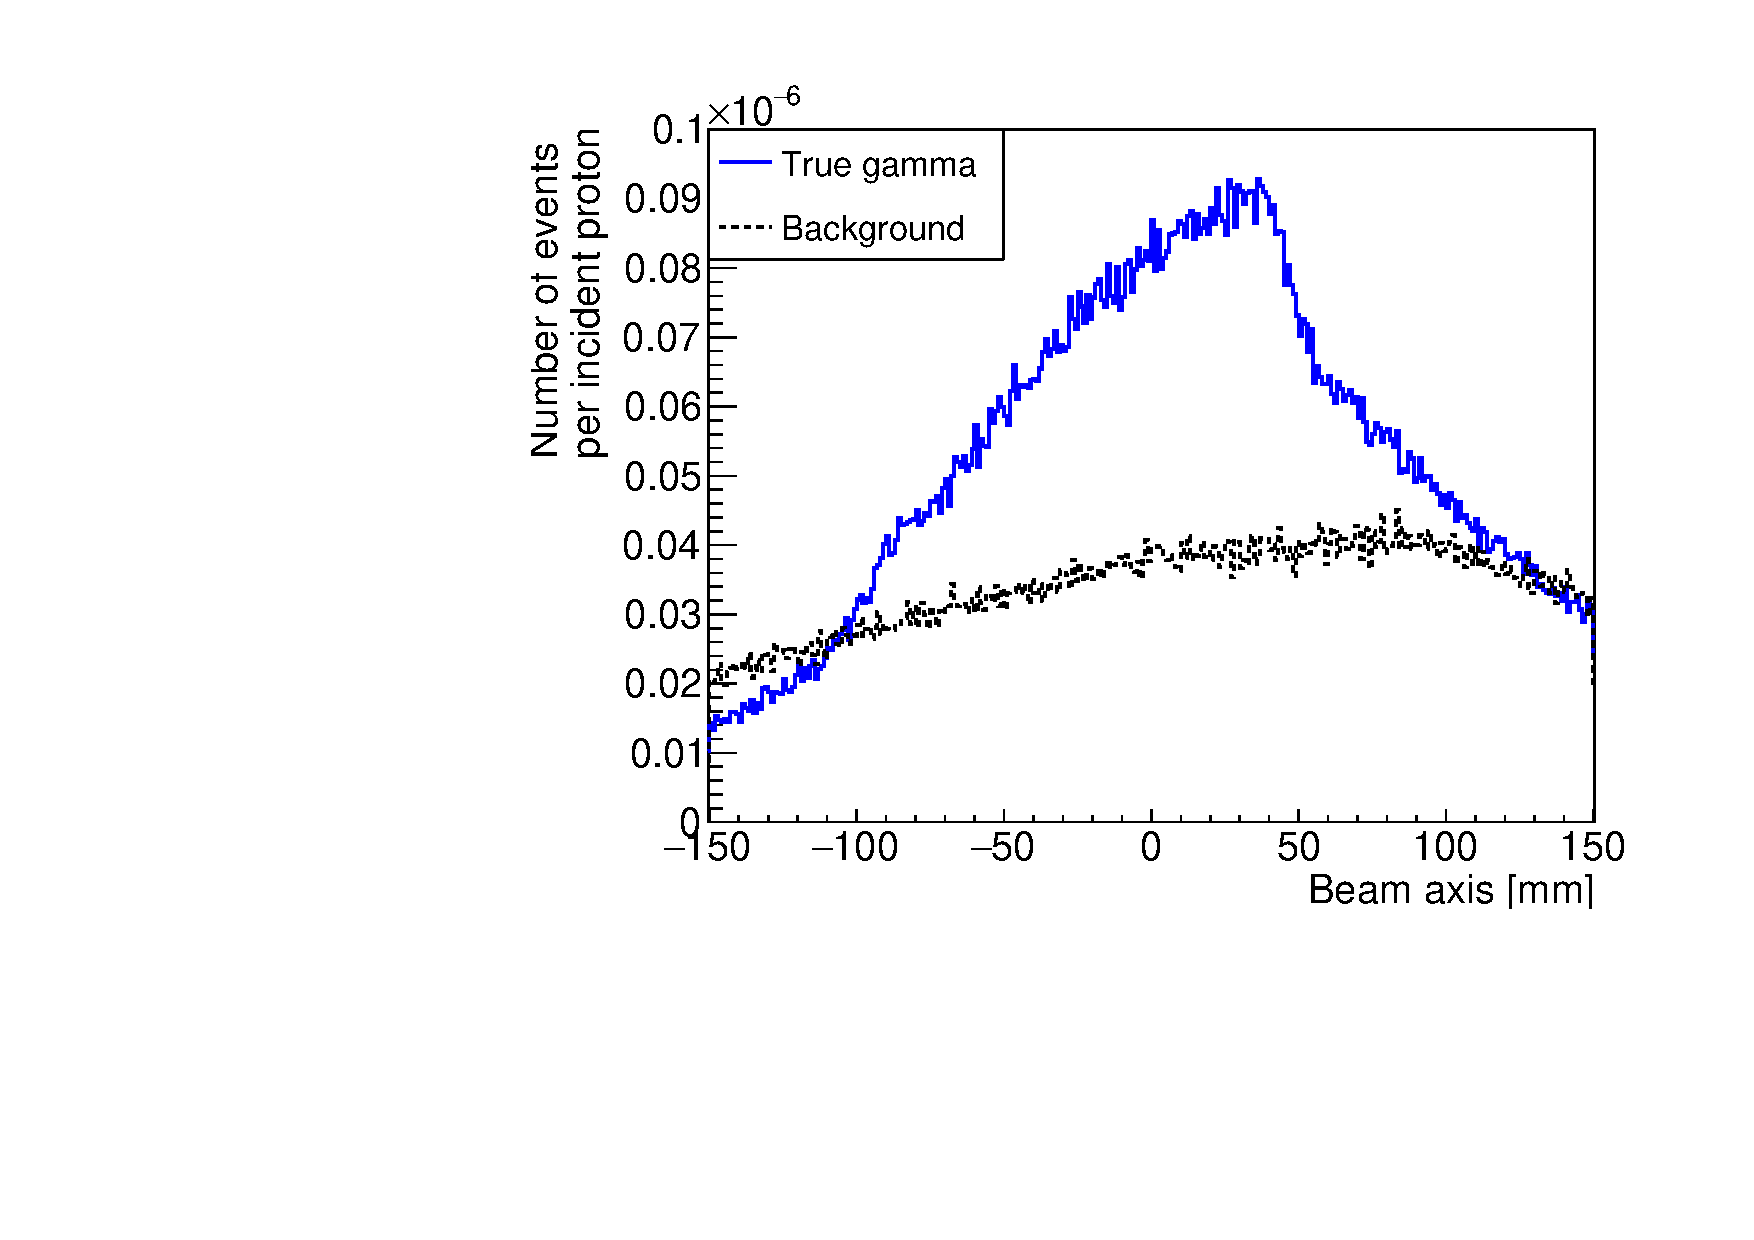
\includegraphics[width=0.33\textwidth]{./Figure/profile_high_stat_linecone_2.pdf}}
% \subfloat[\label{fig:fig_Results_Estimation_Camera_Profil_highStat_CC_simulation_Hadronth_MLEM}]{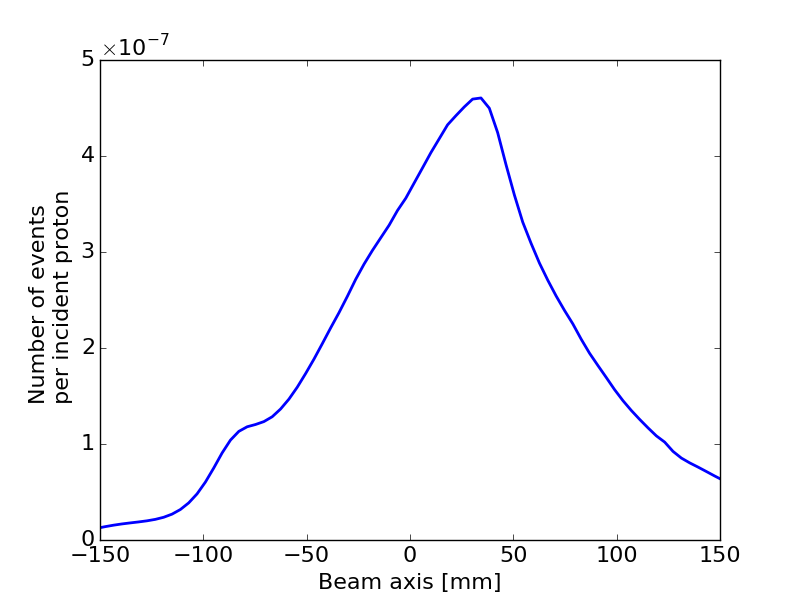
\includegraphics[width=0.32\textwidth]{./Figure/profileY_corr_r15.png}}\\
%  %\subfloat[\label{fig:fig_Estimation_Camera_CC_NURBS_Poisson_LC}]{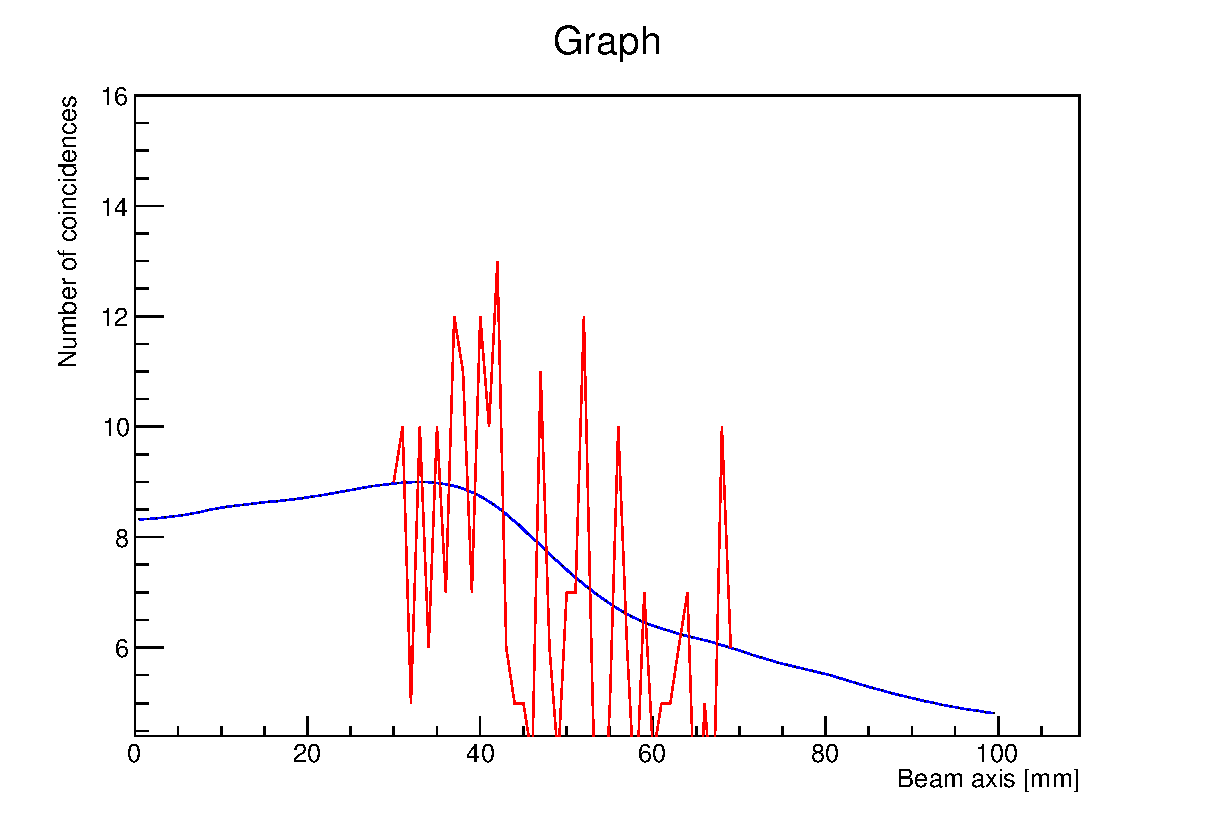
\includegraphics[width=0.33\textwidth]{./Figure/2017-08-02_Poisson_Nurbs_1e8_Article_LC.eps}}
%  \subfloat[\label{fig:fig_Estimation_Camera_CC_NURBS_Poisson_LC}]{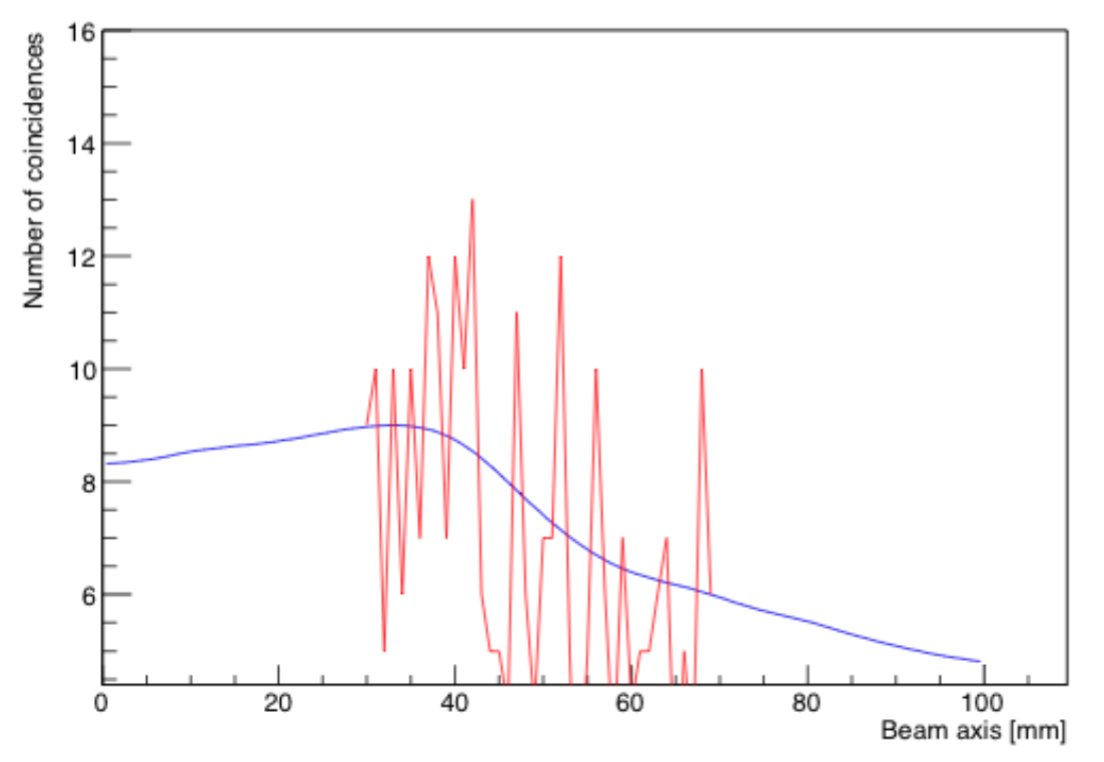
\includegraphics[width=0.33\textwidth]{./Figure/line_cone_NURBS.png}}
%  %\subfloat[\label{fig:fig_Estimation_Camera_CC_NURBS_Poisson_MLEM}]{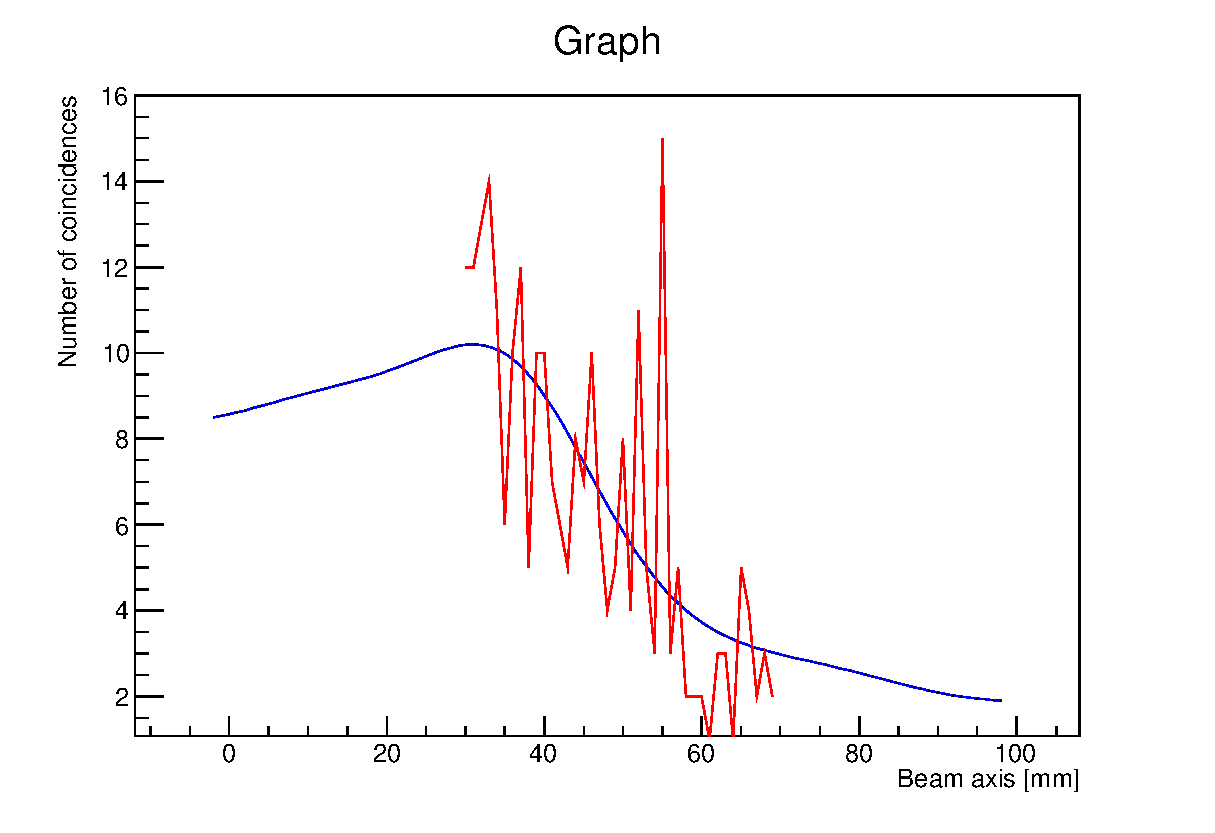
\includegraphics[width=0.33\textwidth]{./Figure/2017-08-02_Nurbs_Poisson_1e8_Article_MLEM.eps}}\\
%  \subfloat[\label{fig:fig_Estimation_Camera_CC_NURBS_Poisson_MLEM}]{\includegraphics[width=0.33\textwidth]{./Figure/MLEM_NURBS.png}}\\
%   %\subfloat[\label{fig:fig_Results_Chi2_Distribution_Variation_CC_simulation_Hadronth_LC}]{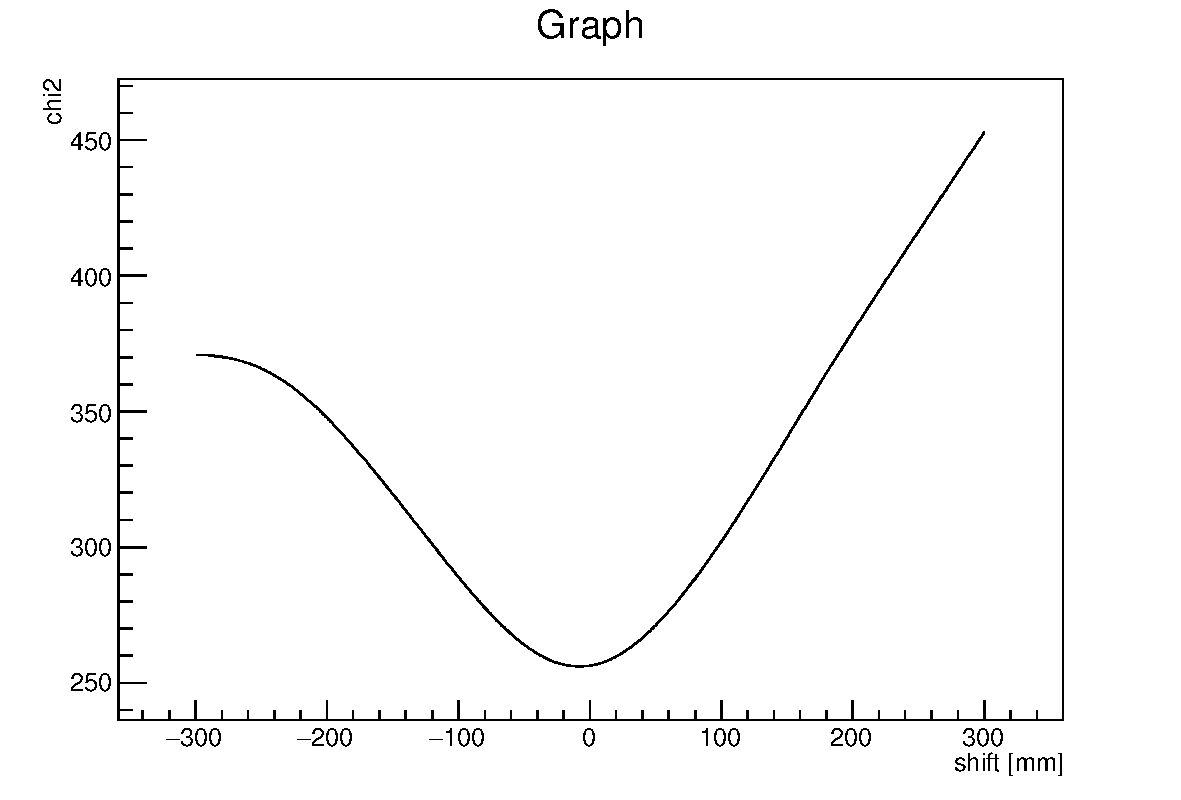
\includegraphics[width=0.33\textwidth]{./Figure/2017-08-02_Distribution_Chi2_1e8_LC.pdf}}
%   \subfloat[\label{fig:fig_Results_Chi2_Distribution_Variation_CC_simulation_Hadronth_LC}]{\includegraphics[width=0.33\textwidth]{./Figure/chi2_linecone.png}}
%  %\subfloat[\label{fig:fig_Results_Chi2_Distribution_Variation_CC_simulation_Hadronth_MLEM}]{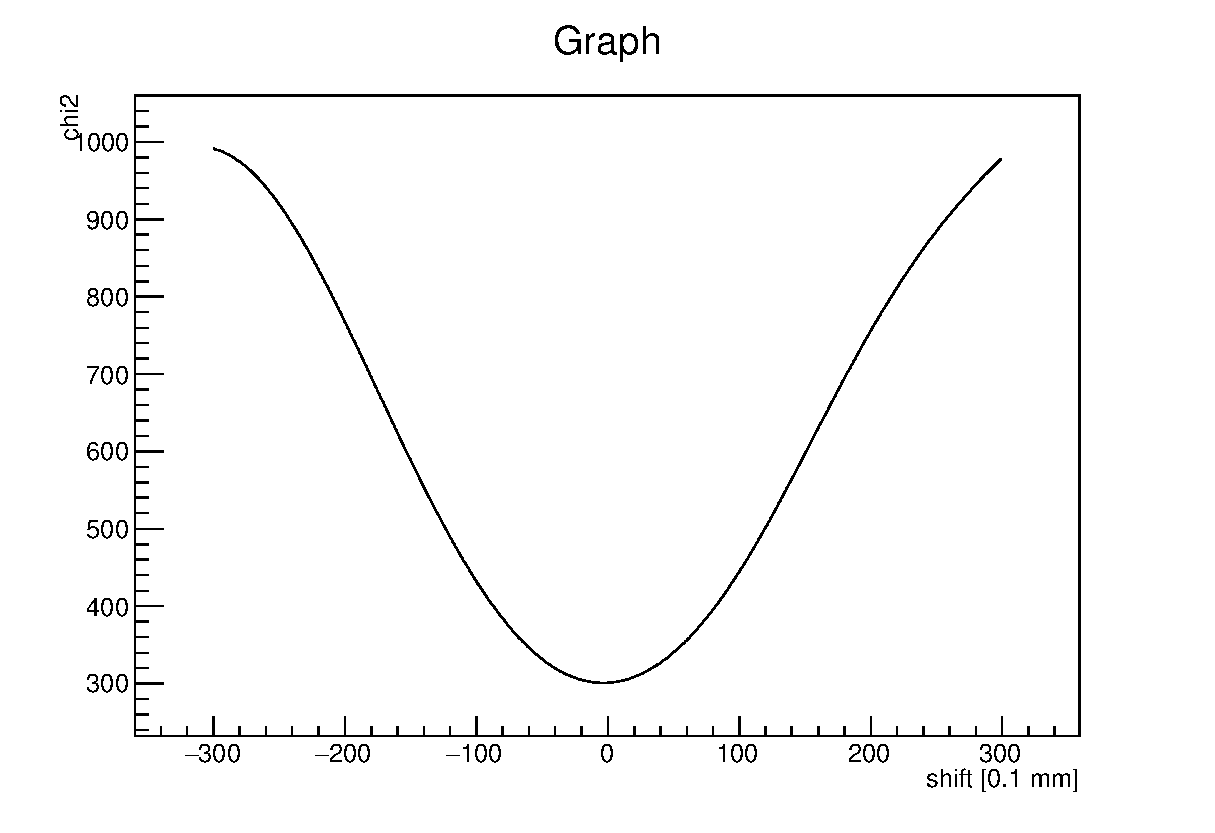
\includegraphics[width=0.33\textwidth]{./Figure/2017-08-02_Distribution_Chi2_Results_binning_1mm_ShiftNurbs0_1mm_1e8_article_MLEM.eps}}\\
%  \subfloat[\label{fig:fig_Results_Chi2_Distribution_Variation_CC_simulation_Hadronth_MLEM}]{\includegraphics[width=0.33\textwidth]{./Figure/chi2_MLEM.png}}\\
%   %\subfloat[\label{fig:fig_Results_Precision_Distribution_Variation_CC_simulation_Hadronth_LC} ]{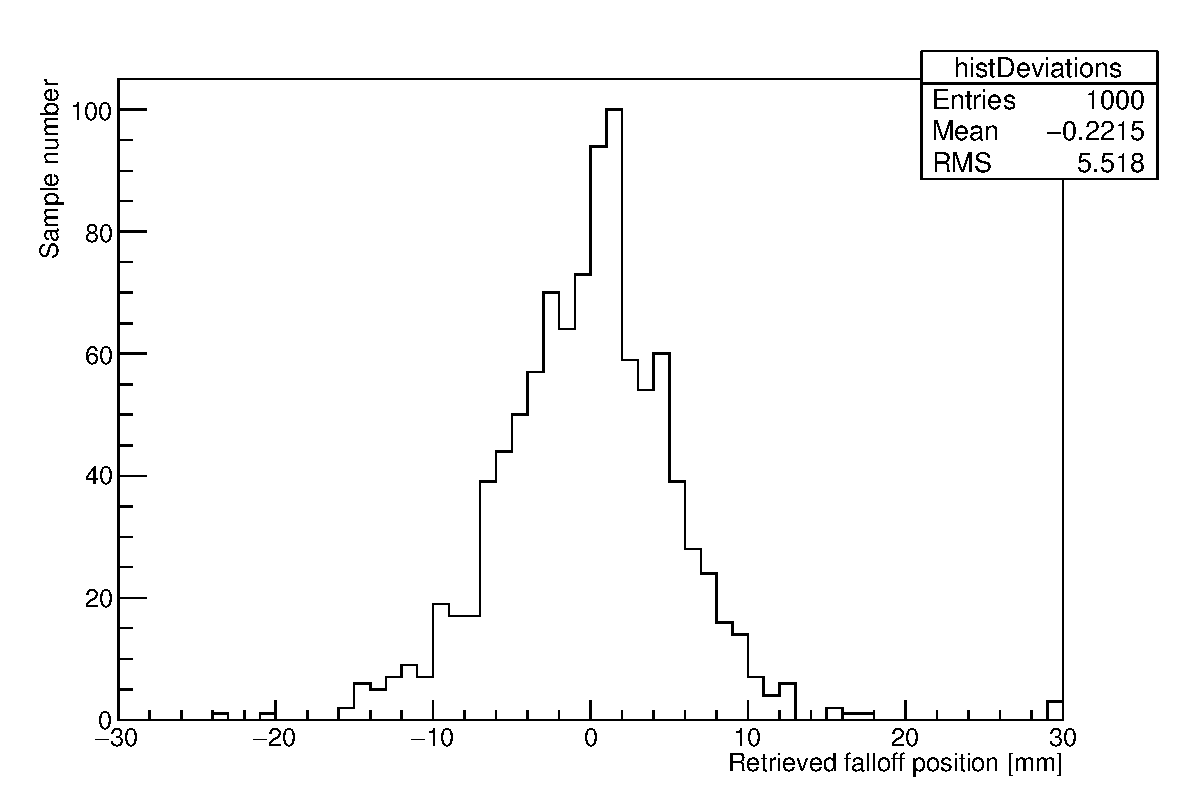
\includegraphics[width=0.33\textwidth]{./Figure/2017-08-02_Distribution_finale_1e8_Article_LC.pdf}}
%   \subfloat[\label{fig:fig_Results_Precision_Distribution_Variation_CC_simulation_Hadronth_LC} ]{\includegraphics[width=0.33\textwidth]{./Figure/deviation_linecone.png}}
%  %\subfloat[\label{fig:fig_Results_Precision_Distribution_Variation_CC_simulation_Hadronth_MLEM} ]{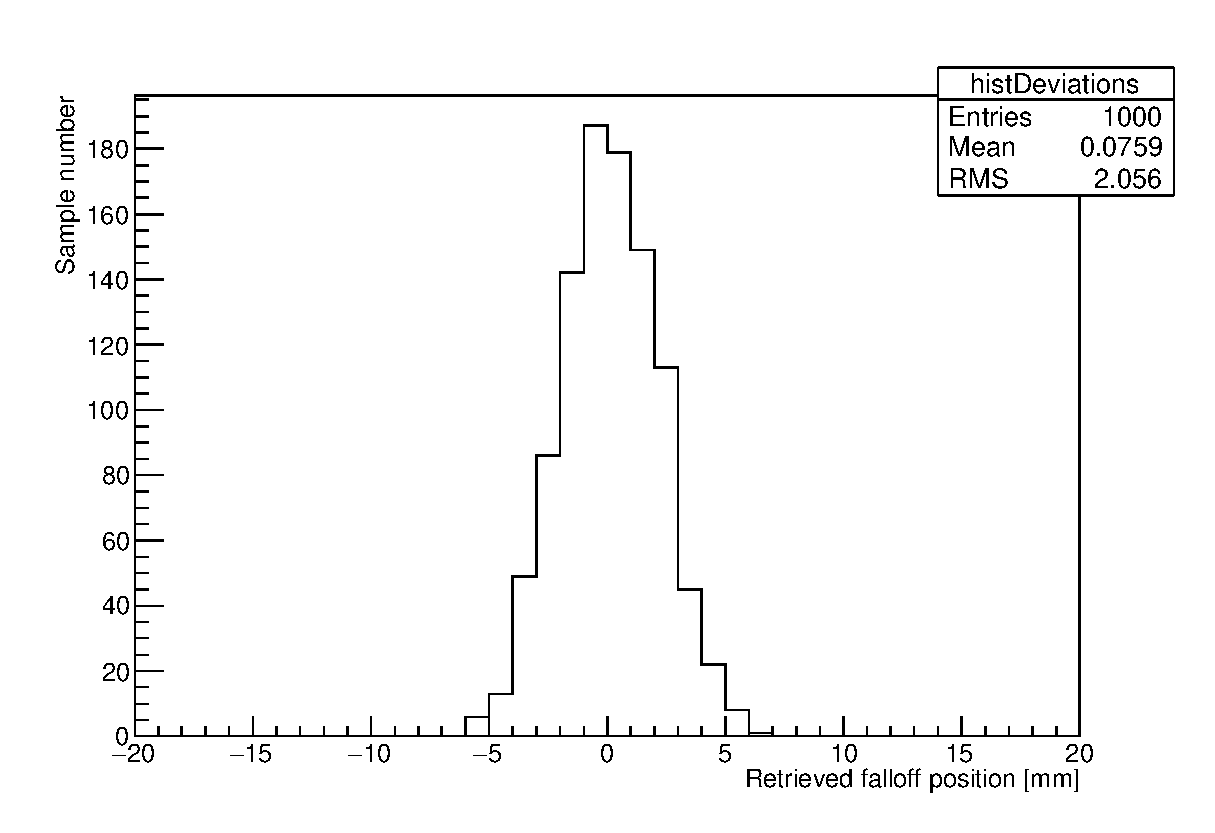
\includegraphics[width=0.33\textwidth]{./Figure/2017-08-02_FallOff_Results_binning_1mm_ShiftNurbs0_1mm_1e8_Article_MLEM.eps}}
%  \subfloat[\label{fig:fig_Results_Precision_Distribution_Variation_CC_simulation_Hadronth_MLEM} ]{\includegraphics[width=0.33\textwidth]{./Figure/deviation_MLEM.png}}
% \caption{Data processing comparison for the same proton simulation with the line cone algorithm (left column) and the LM-MLEM algorithm (right column). The first row gives the reconstructed profile for $10^{10}$ incident protons. The second row shows the reference curve (blue) and the curve obtained with a $10^8$ incident protons subset. The third row shows the $\chi^2$ distribution for one data subset. The last row represents the distribution of the minimal calculated shifts for 1000 subsets at the same statistics of $10^8$ incident protons.}
% \end{figure}

\section{Results}

The possible implementation of the CLaRyS Compton camera as a monitoring system for ion beam therapy has been investigated. The detection efficiency of the camera has been estimated with point-like gamma sources set in different positions with respect to the center of the camera. A PMMA cylindrical phantom has been simulated and exposed to proton and carbon beams at increasing intensities for an analysis of the prompt gamma detection environment (background, random coincidence contamination). The camera precision in the identification of the fall-off of the prompt gamma emission profile has been investigated. For this purpose, the comparison of two different reconstruction methods (line-cone analytical reconstruction and MLEM iterative algorithm) is presented. In the following sections we show the obtained results. 


\subsection{Absolute detection efficiency}
\label{Results::efficiency}

Figure~\ref{fig::efficiency_study} shows the absolute gamma detection efficiency as a function of the gamma source position with respect to the center of the camera in the transverse plane. On the left side, we show the results achieved with an ideal detector. On the right side realistic energy cuts are applied on each detector section: the lower energy limit has been set to 50~keV for the scatterer and 100~keV for the absorber. 

\begin{figure} [!hbtp]	
\centering
%\subfloat[]{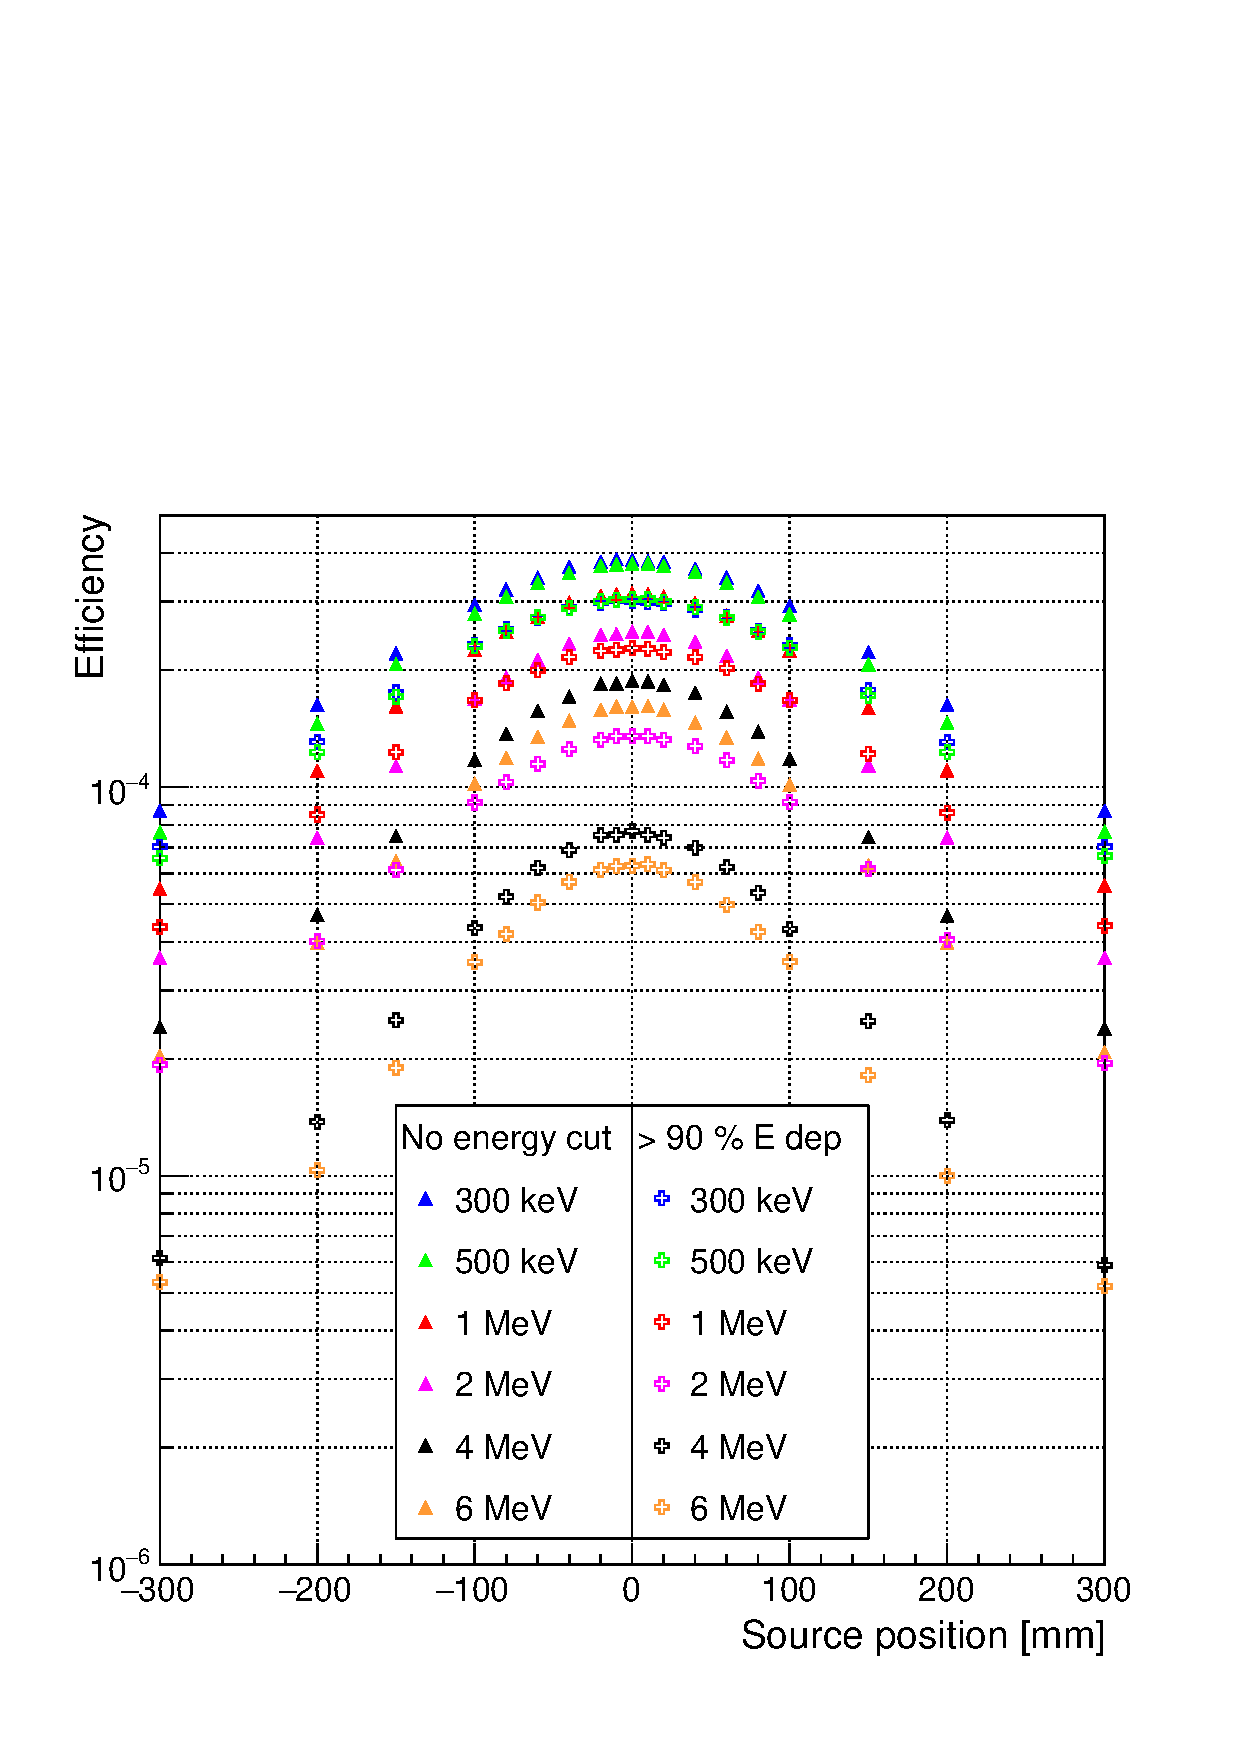
\includegraphics[width=0.5\textwidth]{./Figure/new/EffVSpos_withSumCut.pdf}}
\subfloat[]{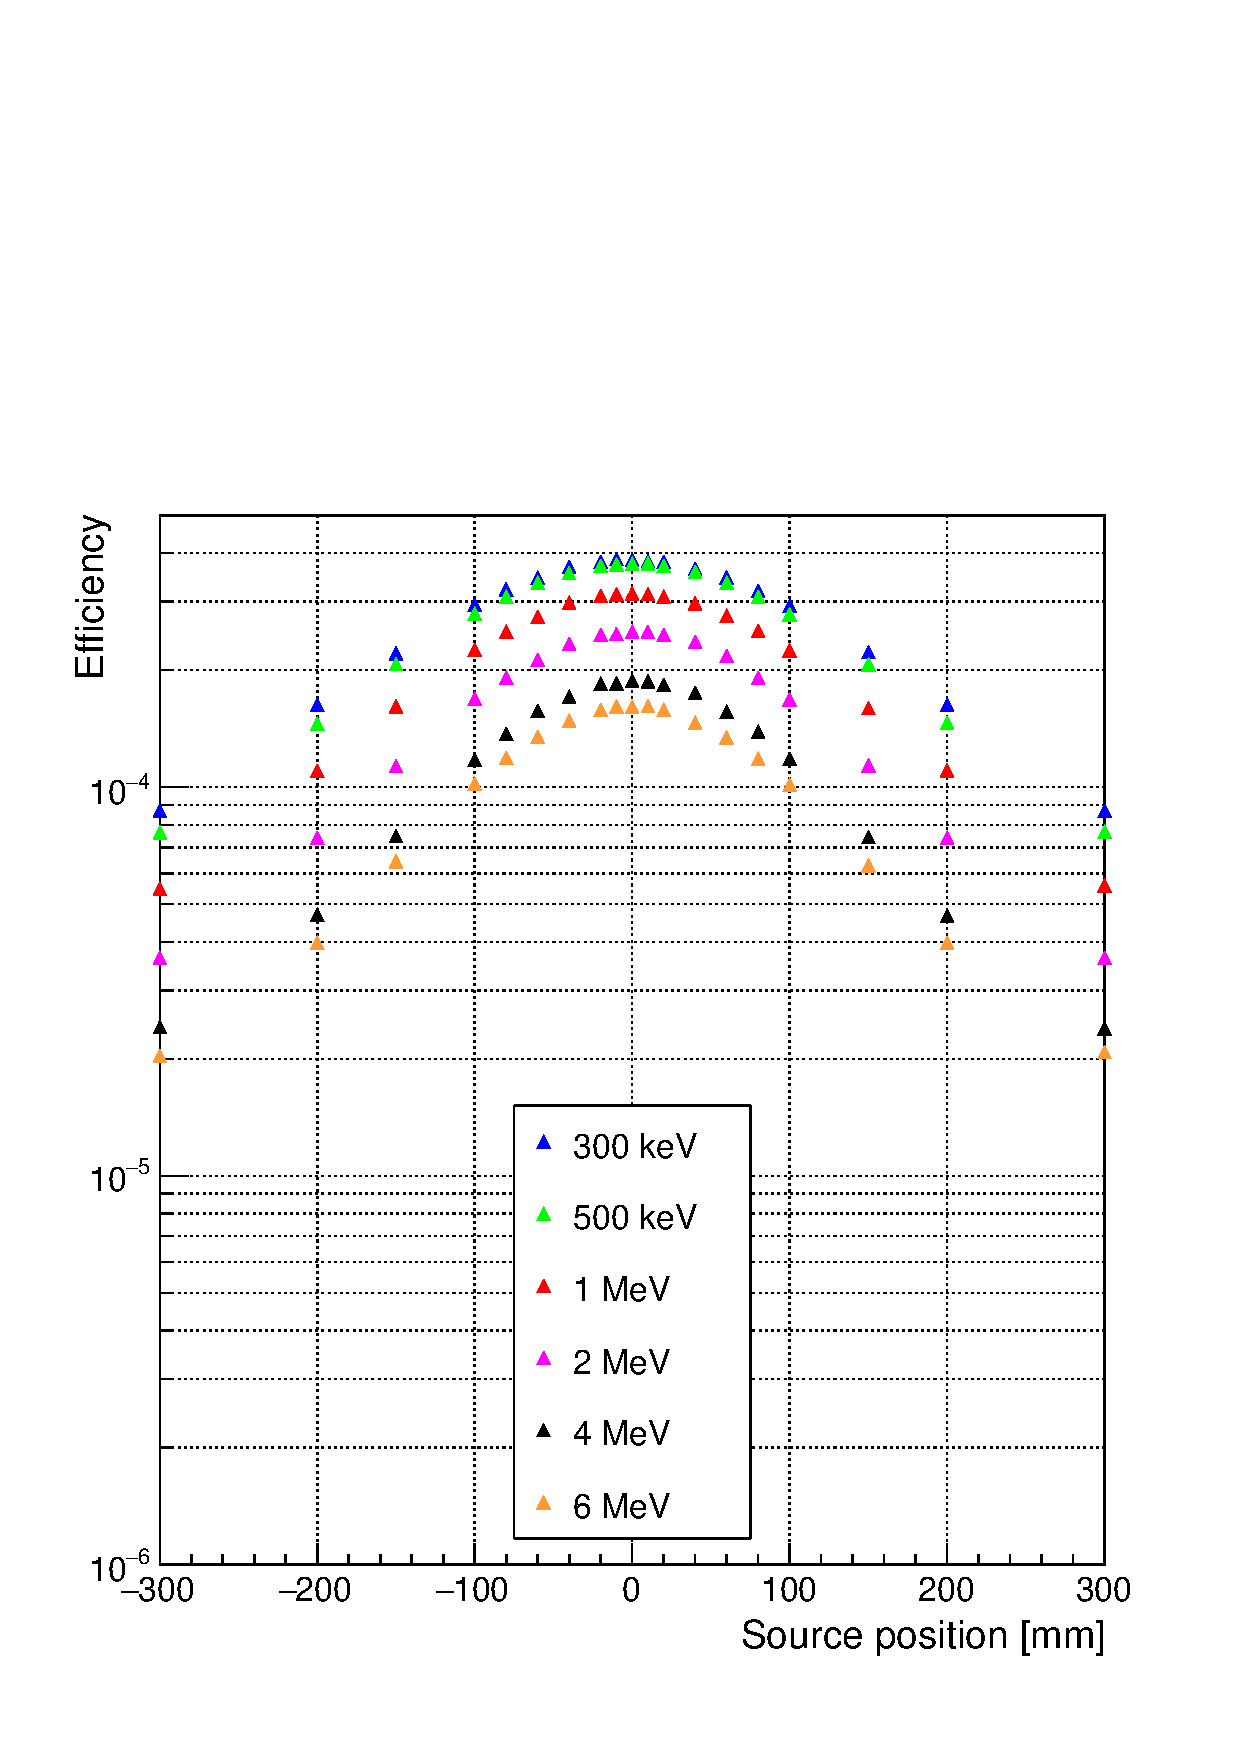
\includegraphics[width=0.5\textwidth]{03_GraphicFiles/chapter3/HT/new/EffVSpos_noCut_simple.pdf}}
%\subfloat[]{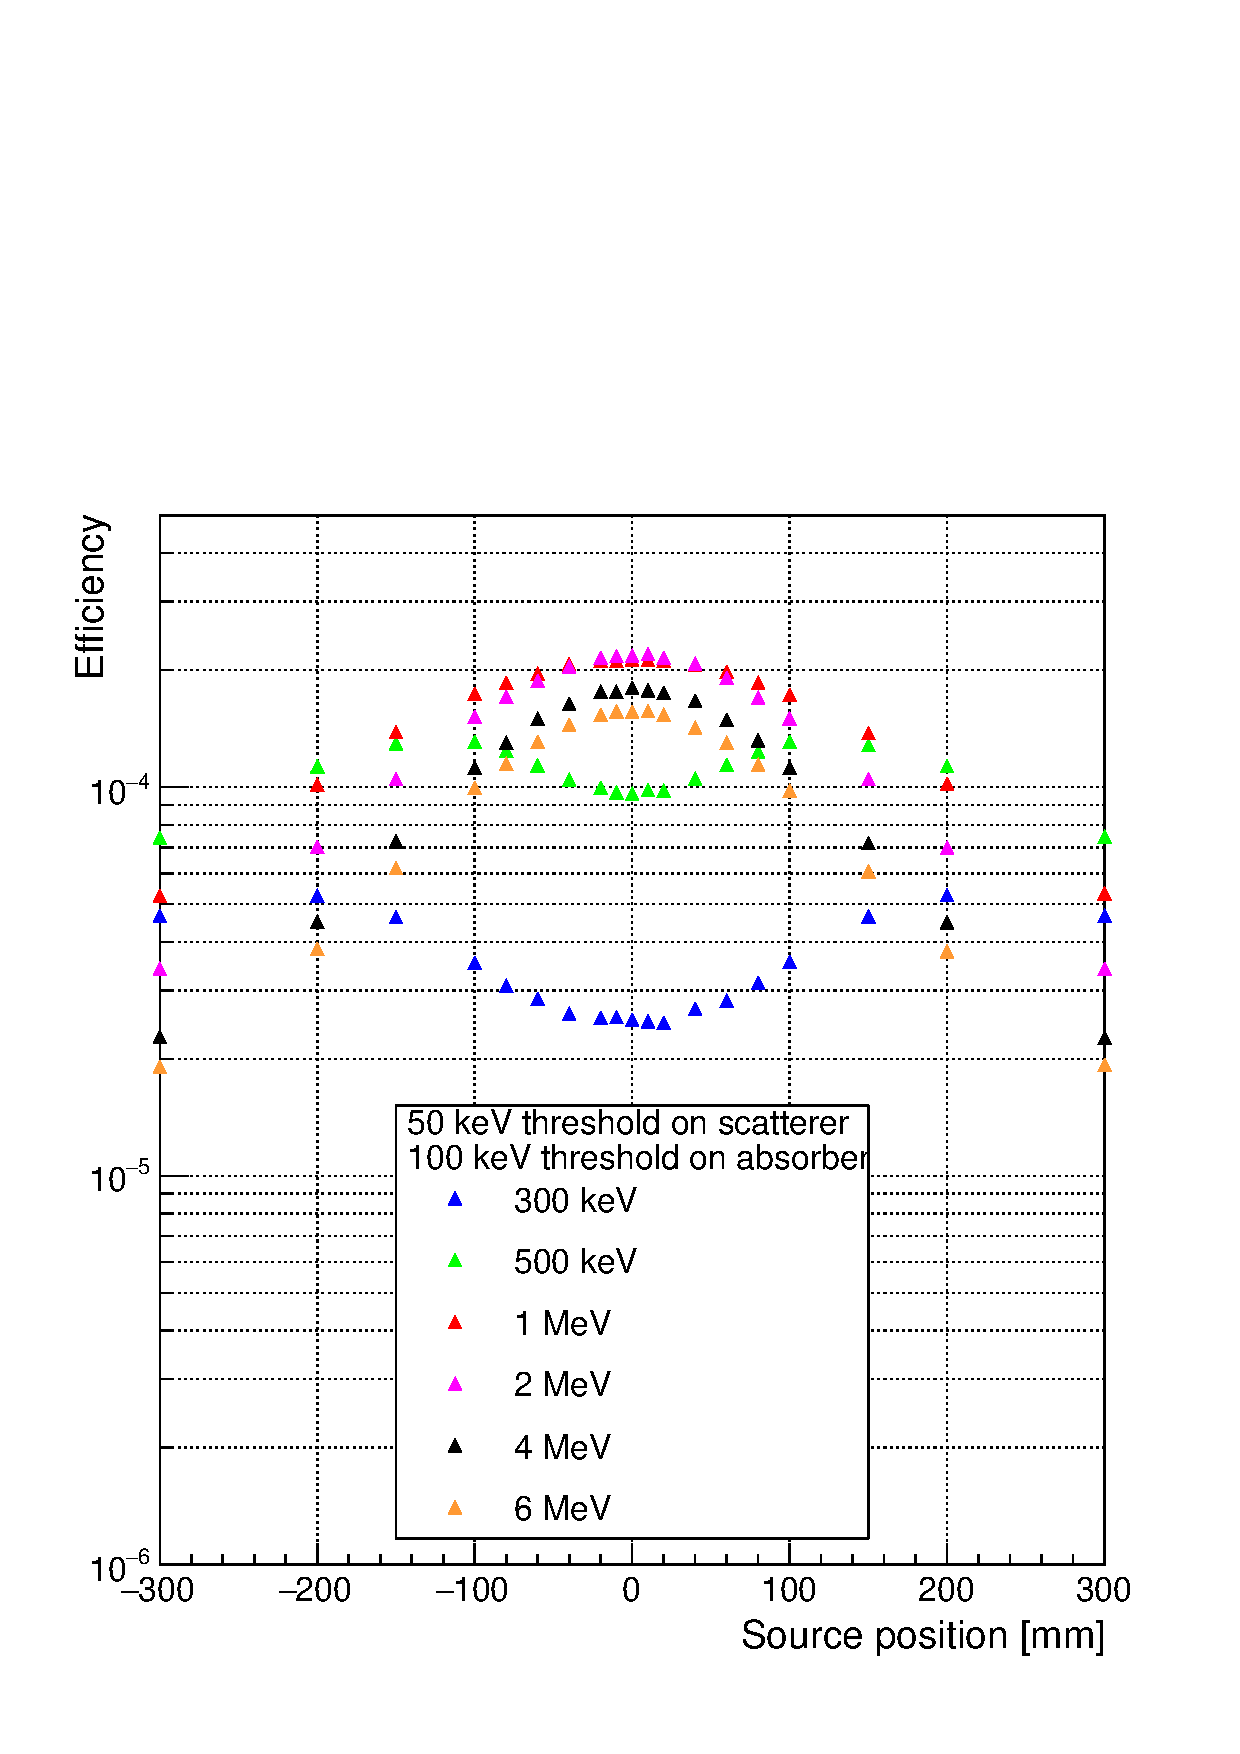
\includegraphics[width=0.5\textwidth]{./Figure/new/EffVSpos_withSingleCut.pdf}}
\subfloat[]{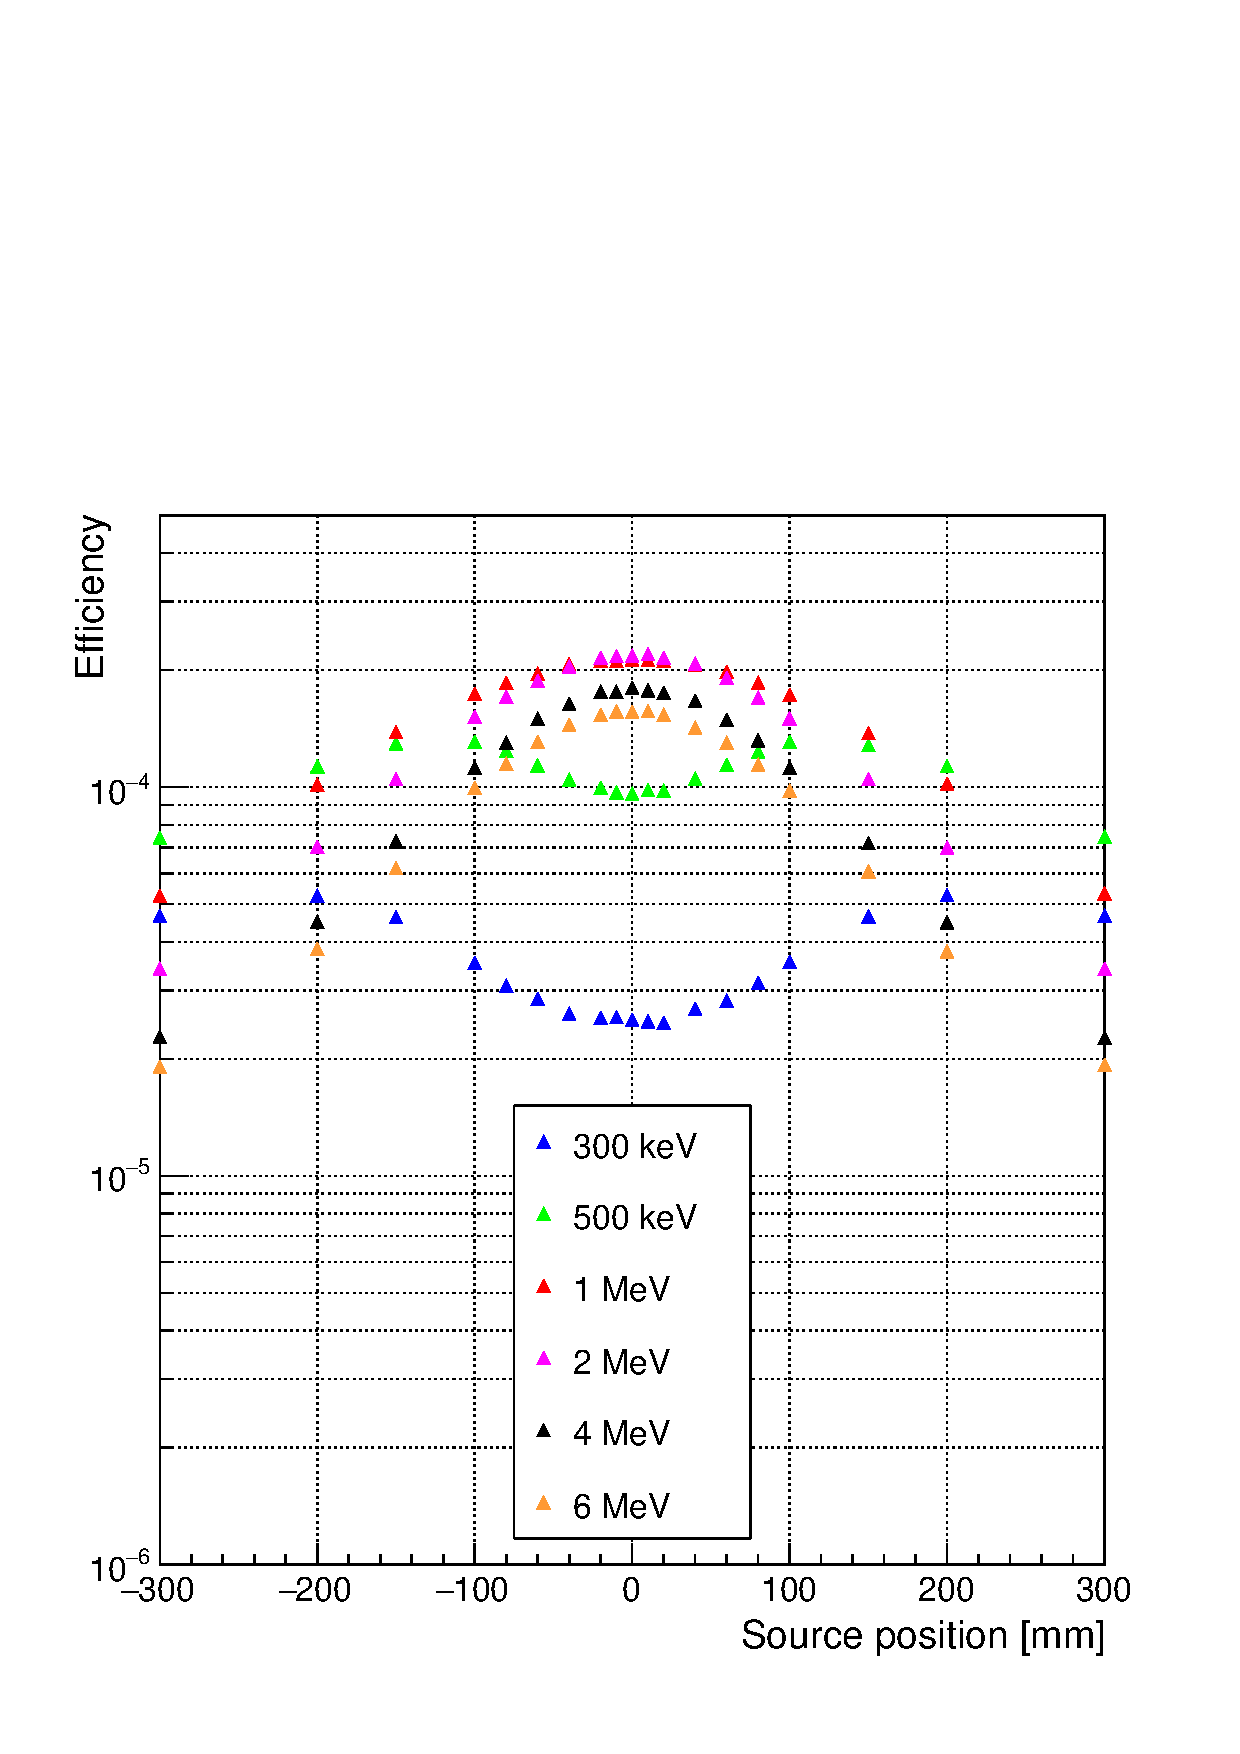
\includegraphics[width=0.5\textwidth]{03_GraphicFiles/chapter3/HT/new/EffVSpos_CutSingle_simple.pdf}}
\caption{Absolute Compton camera efficiency as a function of the gamma source position for different gamma energies, in the range between 300~keV to 6~MeV. The left side shows the camera efficiency with no data selection. In the right side, detection energy thresholds are applied: the lower energy thresholds are set to 
50~keV for the scatterer and 100~keV for the absorber, to reproduce a realistic scenario. These values can change for the final configuration, according to the detector energy resolutions achieved.}
\label{fig::efficiency_study}
\end{figure}

As expected according to the interaction probability energy dependency, the efficiency is higher for low gamma energies, and it lies in the range $4\times10^{-4}$ at 300~keV and $1.5\times10^{-4}$ at 6~MeV at the center of the camera. Moreover, it can be noticed how the efficiency slightly drops as the point source is shifted away from the camera center: efficiency reductions at 500~keV and 4~MeV are respectively of 25\% and 35\%. This effect is more important for high energies, for which the incident gamma is less deflected in the scatterer for the same energy deposited compared to a low energy gamma (see equation~\ref{Compton_equation}).\\  
Figure~\ref{fig::efficiency_study}(b) shows the effect of realistic camera detection thresholds as opposed to ideal detection. The gamma detection efficiency drops of a factor ranging from about 1.25 to more than an order of magnitude for the central detection area for energies in the range 300~keV - 2~MeV respectively. The effect is reduced by the distance of the source from the center of the camera. Negligible effects are detected for positions with a distance greater than 200~mm from the center of the camera, and for any distance at energies above 2~MeV, while the efficiency is reduced in the central area of the camera.\\

\begin{figure} [!hbtp]	
\centering
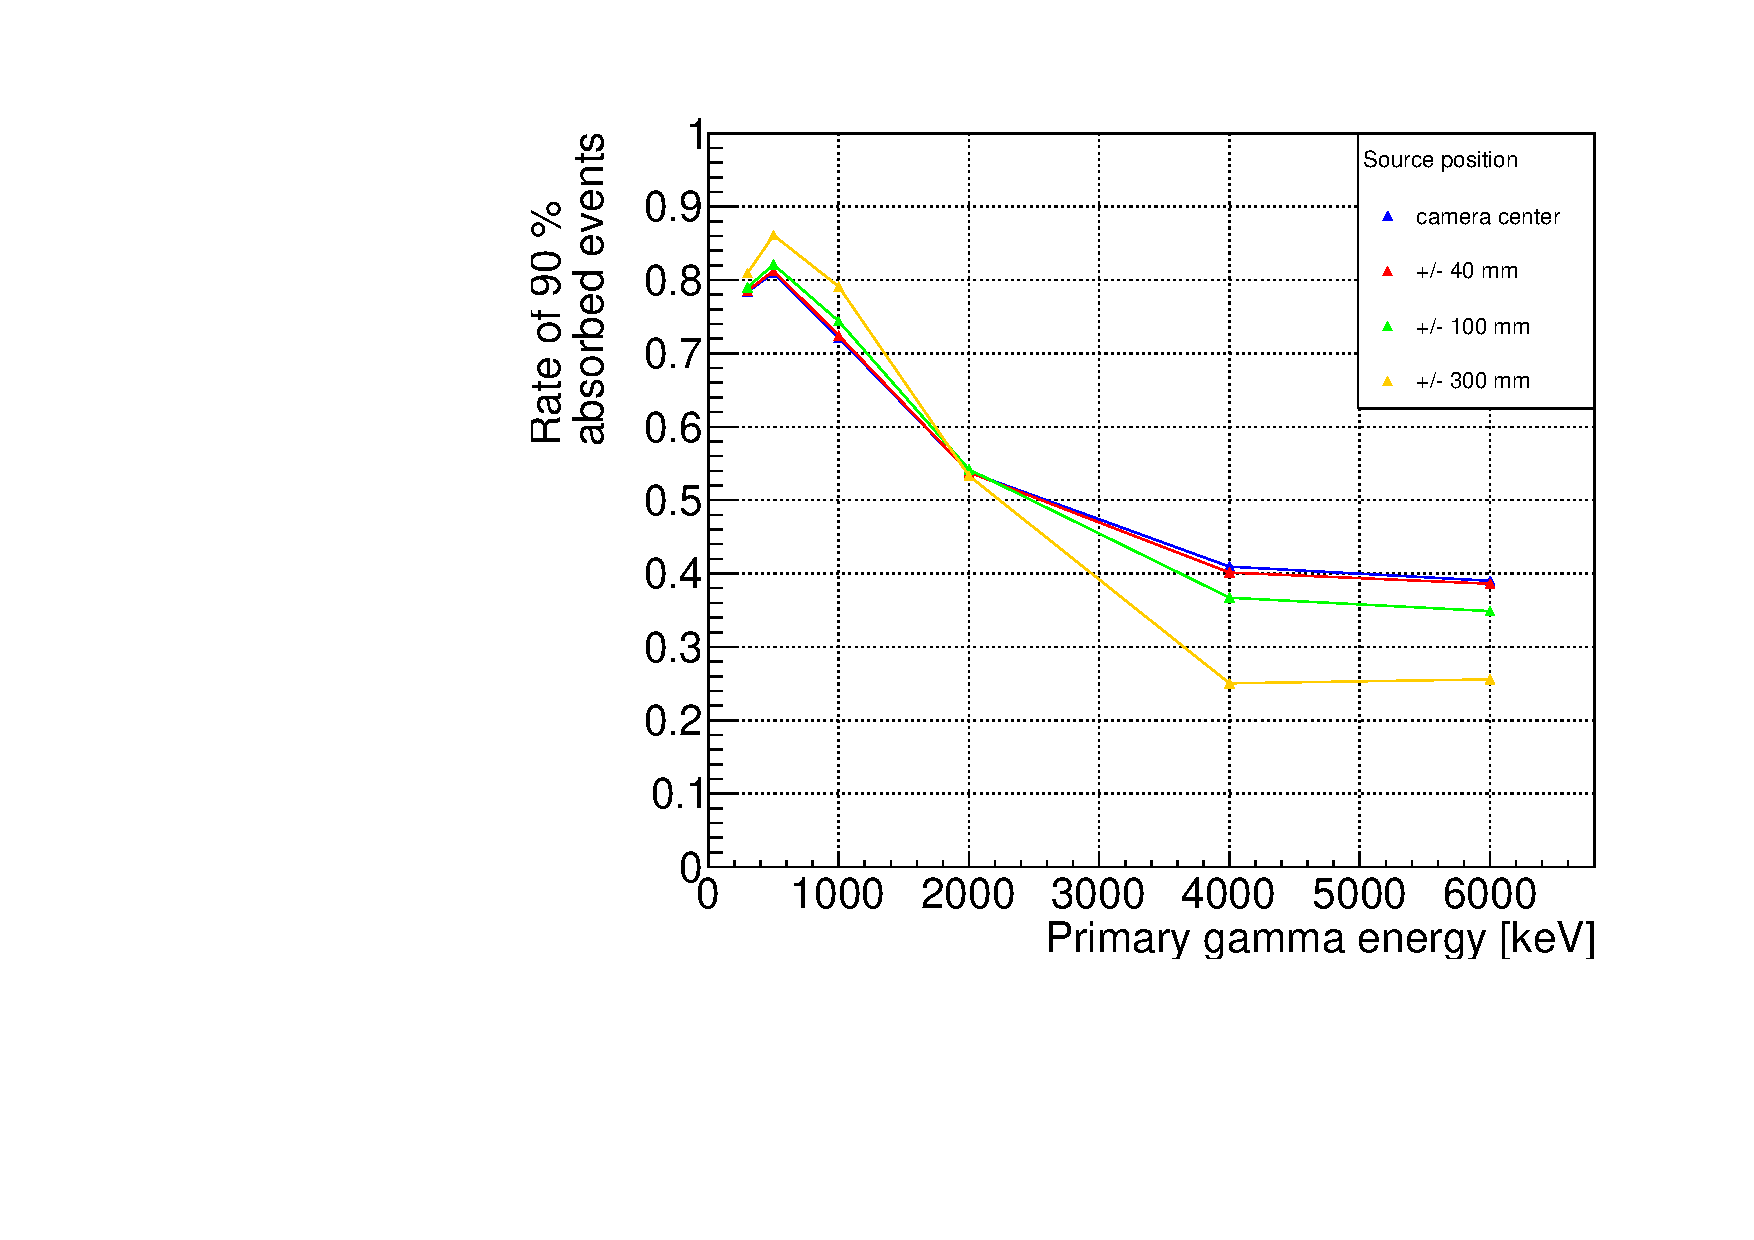
\includegraphics[width=0.5\textwidth]{03_GraphicFiles/chapter3/HT/new/rate_90percent_energy_4distances.pdf}
\caption{Ratio between coincidence events with more than 90\% of the primary photon energy absorbed in the detector layer and all detected coincidences for 4 source positions: center of the camera, 40, 100, 300~mm from the center.}
\label{fig::rate_full_abs}
\end{figure}


Figure~\ref{fig::rate_full_abs} shows the rate of events with more than 90\% of the primary gamma energy deposited in the detector layers, for 4 different source positions (center of the camera, 40, 100, 300~mm far from the center) with no selection applied on a single detector layer basis. As expected, the rate of almost fully absorbed events decreases as the energy increases, in a range between more than 80\% and 40\% for 300~keV and 6~MeV primary photon energy, respectively, with the source at the center of the camera. Also the source position has an impact, with a 35\% reduction if moving from the center to a distance of 300~mm in the transverse plane. For lower energies, the rate of fully absorbed events slightly increases when the source is moving away from the camera center, with maximum variations of less than 10\%. 
 

\subsection{Rate of random coincidences}
\label{Results::beamInt}
 
In figure~\ref{fig:coincidences}, the different components of the signal resulting from the PMMA exposure to proton and carbon ion beams are shown as a function of the beam intensity. The true coincidences represent scatterer-absorber time coincidences generated by the same gamma ray. All the other coincidence types compose the background. The collected data sets are reported with and without the applied time-of-flight discrimination, mainly employed for neutron rejection, as mentioned in section~\ref{MatMeth::TOF_Ecut}.


\begin{figure} [!h]
  %\subfloat[]{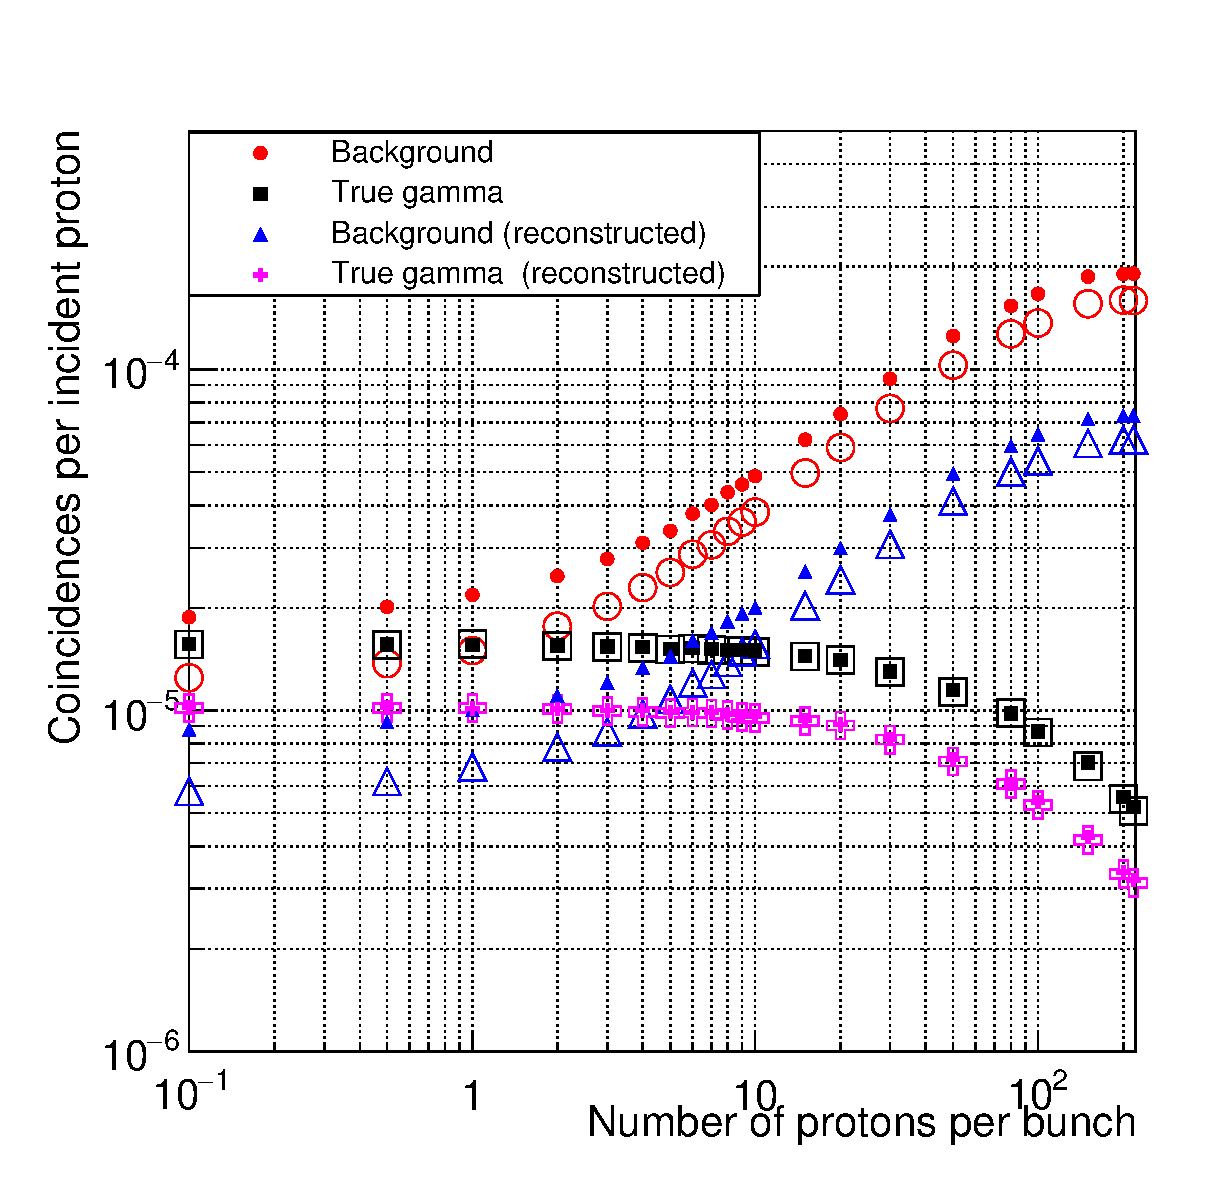
\includegraphics[width=0.5\textwidth]{./Figure/2017_06_28_Taux_coincidences_variation_protons_New_design_4EntreesLegend_LogXLogY.eps}}
  \subfloat[]{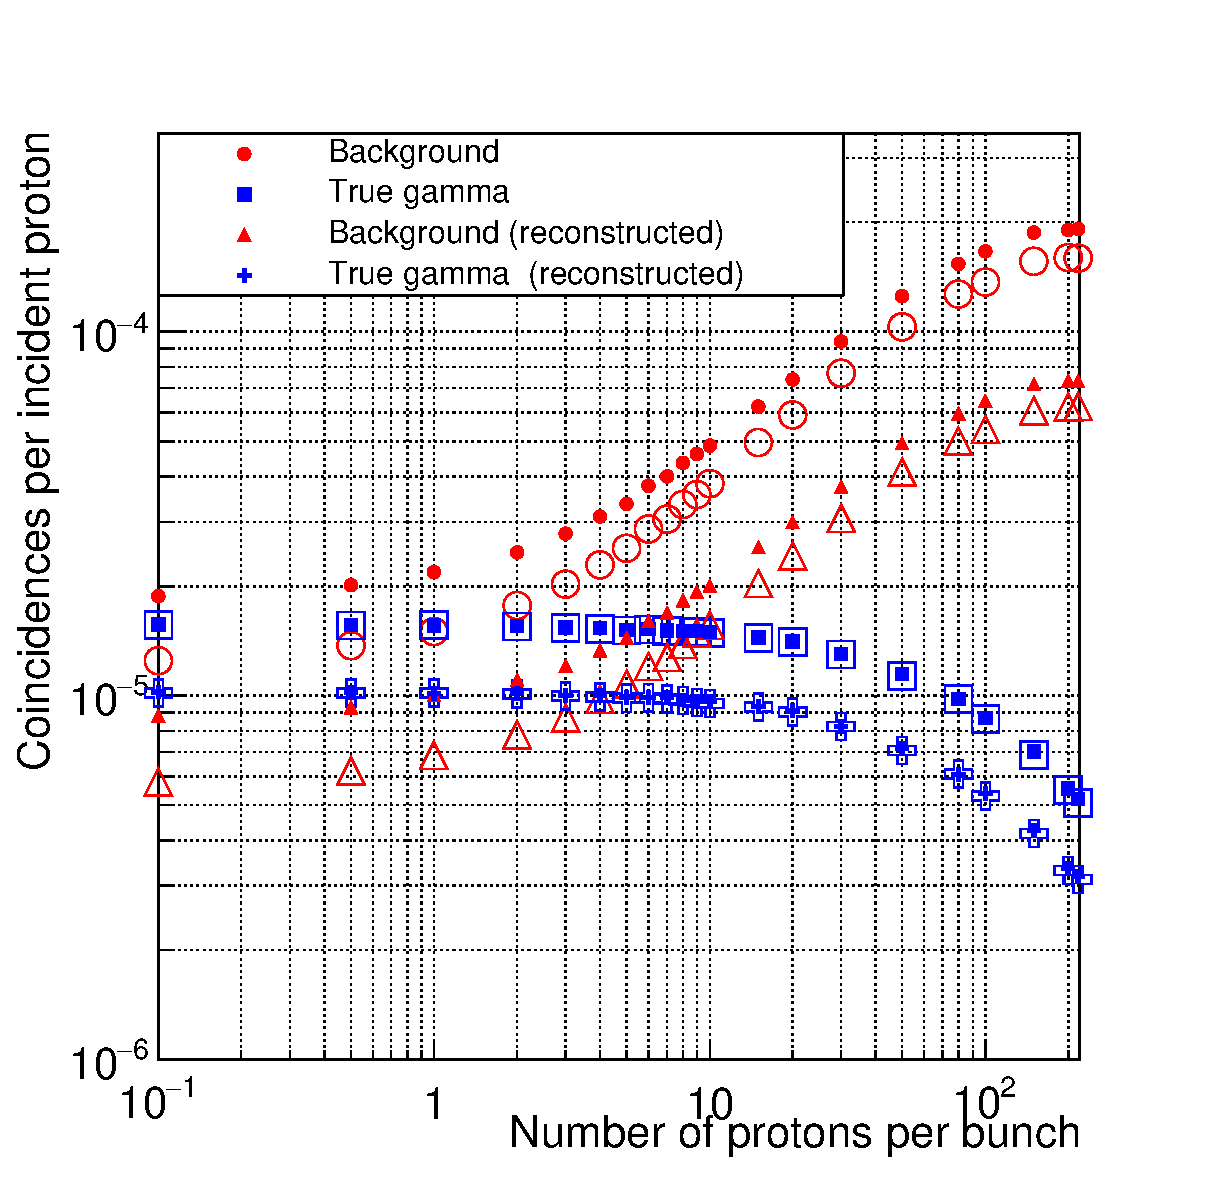
\includegraphics[width=0.5\textwidth]{03_GraphicFiles/chapter3/HT/new/coincYields_protons.eps}}
  %\subfloat[]{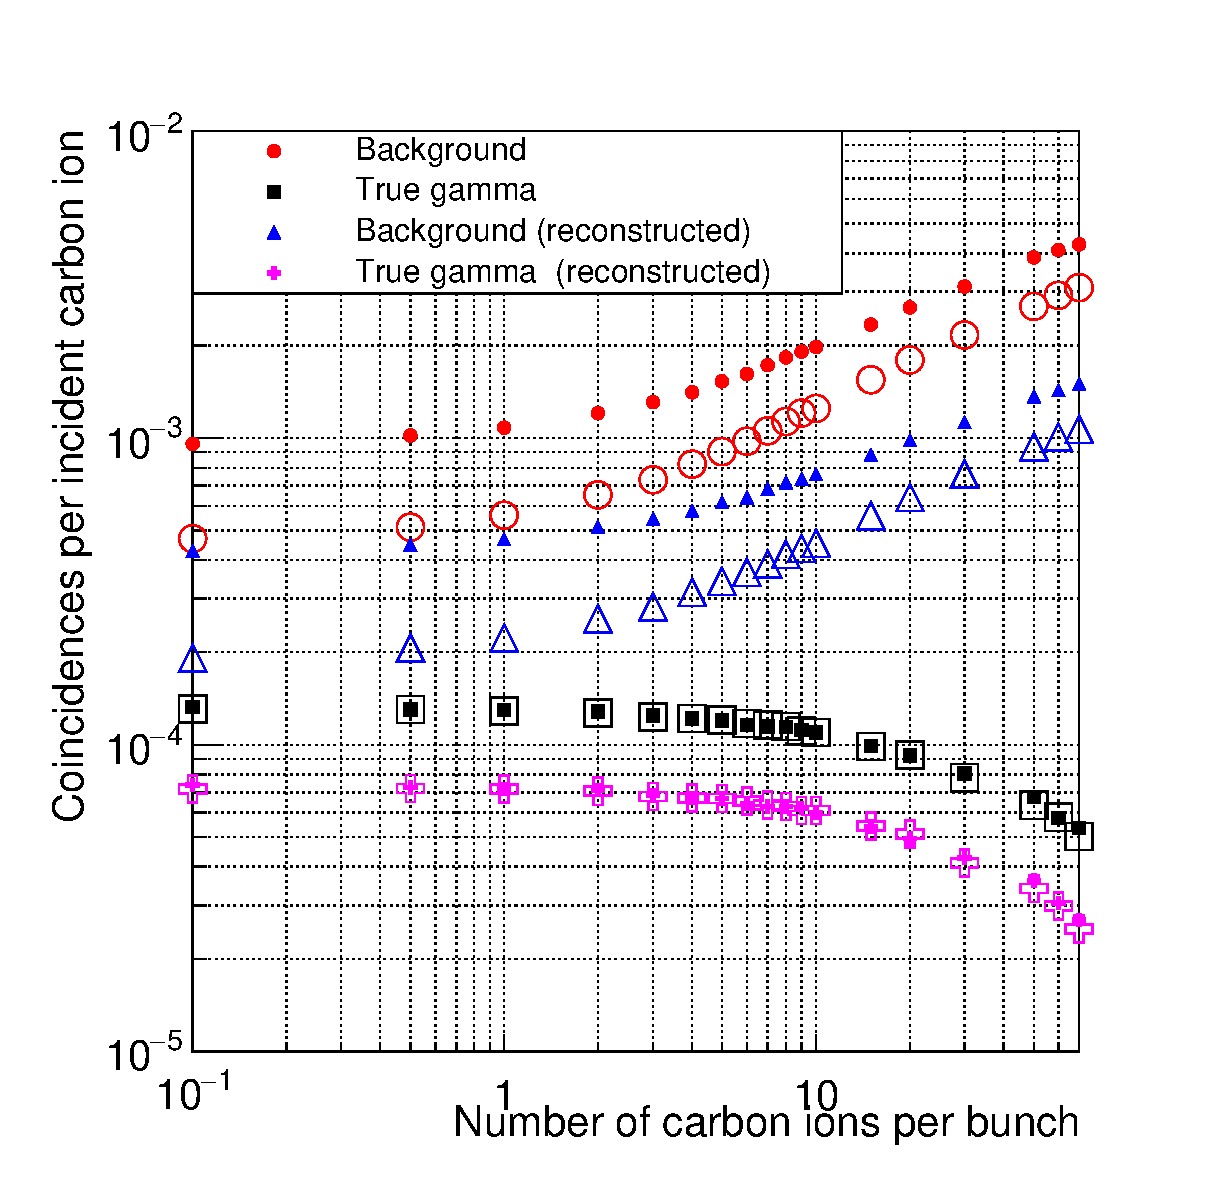
\includegraphics[width=0.5\textwidth]{./Figure/2017_06_28_Taux_coincidences_variation_carbonIons_New_design_4EntreesLegend_LogXLogY.eps}}
  \subfloat[]{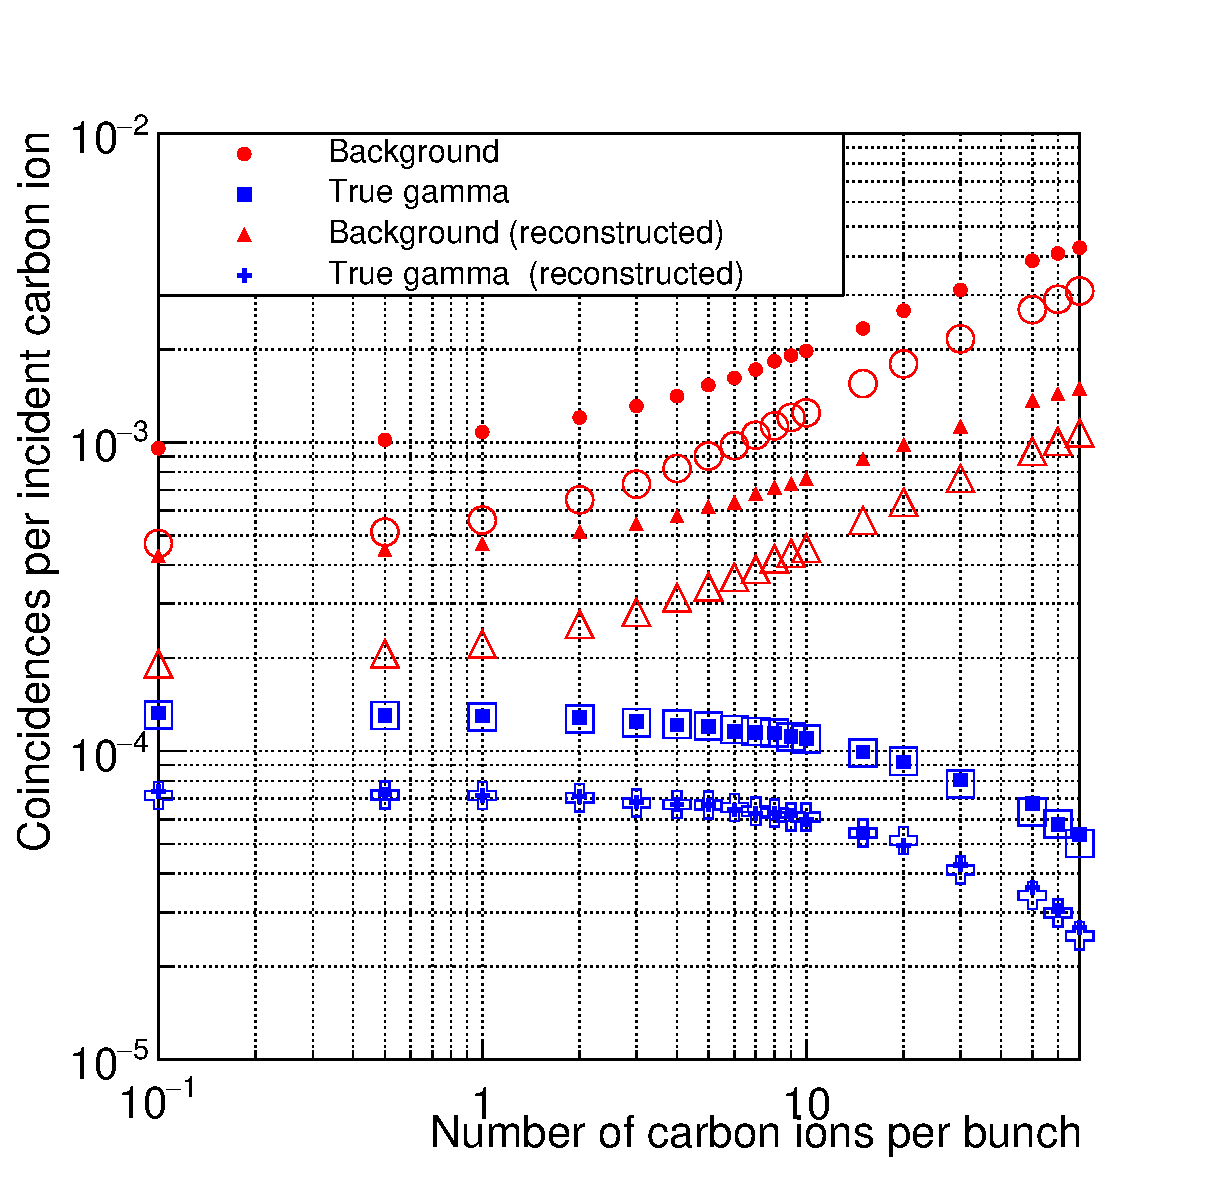
\includegraphics[width=0.5\textwidth]{03_GraphicFiles/chapter3/HT/new/coincYields_Cions.eps}}
  \caption{Coincidences yield for protons (left) and carbon ions (right) as a function of the beam intensity. The intensity is reported as number of incident particles per bunch. The filled markers correspond to the collected data without time-of-flight discrimination, while this cut is applied to the data reported with empty markers. Moreover, the yields are given before and after the profile reconstruction with the line-cone algorithm.}
  \label{fig:coincidences}
\end{figure}

In figure~\ref{fig:coincidences}(a) and (b) the amount of true gamma coincidences and background events are reported before and after reconstruction via line-cone algorithm as a function of the beam intensity for proton (a) and carbon ion (b) beams. In addition to this, for each curve realized with the complete collected data set, the related one realized after time-of-flight selection of events is sketched (empty symbols). All the curves have been normalized to the number of incident ions.

The amount of background events (mainly random coincidences) increases with the increasing beam intensity: a factor of about 30 with respect to true gamma events is obtained for proton beams at  the intensity of 200 protons per bunch with no event selection, while a factor more than two times higher is reported for carbon ions in the same conditions. The time-of-flight selection can slightly improve the signal -over-noise ratio by reducing the amount of background events. The amount of true gamma events and background events becomes similar at the intensity of about 1 proton per bunch.


\subsection{Camera precision}
\label{Results::precision_reconstruction}
Given the results presented in the previous section, the camera precision in the fall-off identification is investigated with proton beams at reduced intensities.
%The simulation setup shown in figure~\ref{fig:fig_setup_CC_simulation_Hadronth} has been implemented to test the line-cone analytic reconstruction method and compare it to the iterative LM-MLEM algorithm~\cite{maxim_filtered_2014,hilaire_compton_2014}. 
A single data set has been collected, corresponding to the irradiation of the PMMA phantom with a proton 160~MeV monoenergetic beam, with a reduced intensity of 1 proton per bunch. A total of $10^{10}$ protons has been simulated to define the reference PG profile, and then different low statistics profiles have been produced for the precision estimate as explained in section~\ref{MatMeth:precision}. 

The high statistics profile reconstructed via line-cone algorithm is shown in figure~\ref{fig:fig_Results_Estimation_Camera_Profil_highStat_CC_simulation_Hadronth_LineCone} and via the LM-MLEM reconstruction method in figure~\ref{fig:fig_Results_Estimation_Camera_Profil_highStat_CC_simulation_Hadronth_MLEM}. A NURBS model of a low statistics sample ($10^8$ incident protons) is shown in figures~\ref{fig:fig_Estimation_Camera_CC_NURBS_Poisson_LC} for the line cone and~\ref{fig:fig_Estimation_Camera_CC_NURBS_Poisson_MLEM} for the MLEM.
Figures~\ref{fig:fig_Results_Chi2_Distribution_Variation_CC_simulation_Hadronth_LC} and~\ref{fig:fig_Results_Chi2_Distribution_Variation_CC_simulation_Hadronth_MLEM} show the distribution of $\chi^2$ calculated for a low statistic profile at $10^8$ incident protons. The retrieved optimal shift distribution is shown in figure~\ref{fig:fig_Results_Precision_Distribution_Variation_CC_simulation_Hadronth_LC} and~\ref{fig:fig_Results_Precision_Distribution_Variation_CC_simulation_Hadronth_MLEM} for the line-cone and LM-MLEM algorithm respectively, for $10^8$ incident protons as well.
Figure~\ref{fig:comparison} shows the results of the reconstruction of the profile obtained with 10$^8$ primary protons.


\begin{figure}
  \centering
  %\subfloat[\label{fig:fig_Results_Estimation_Camera_Profil_highStat_CC_simulation_Hadronth_LineCone}]{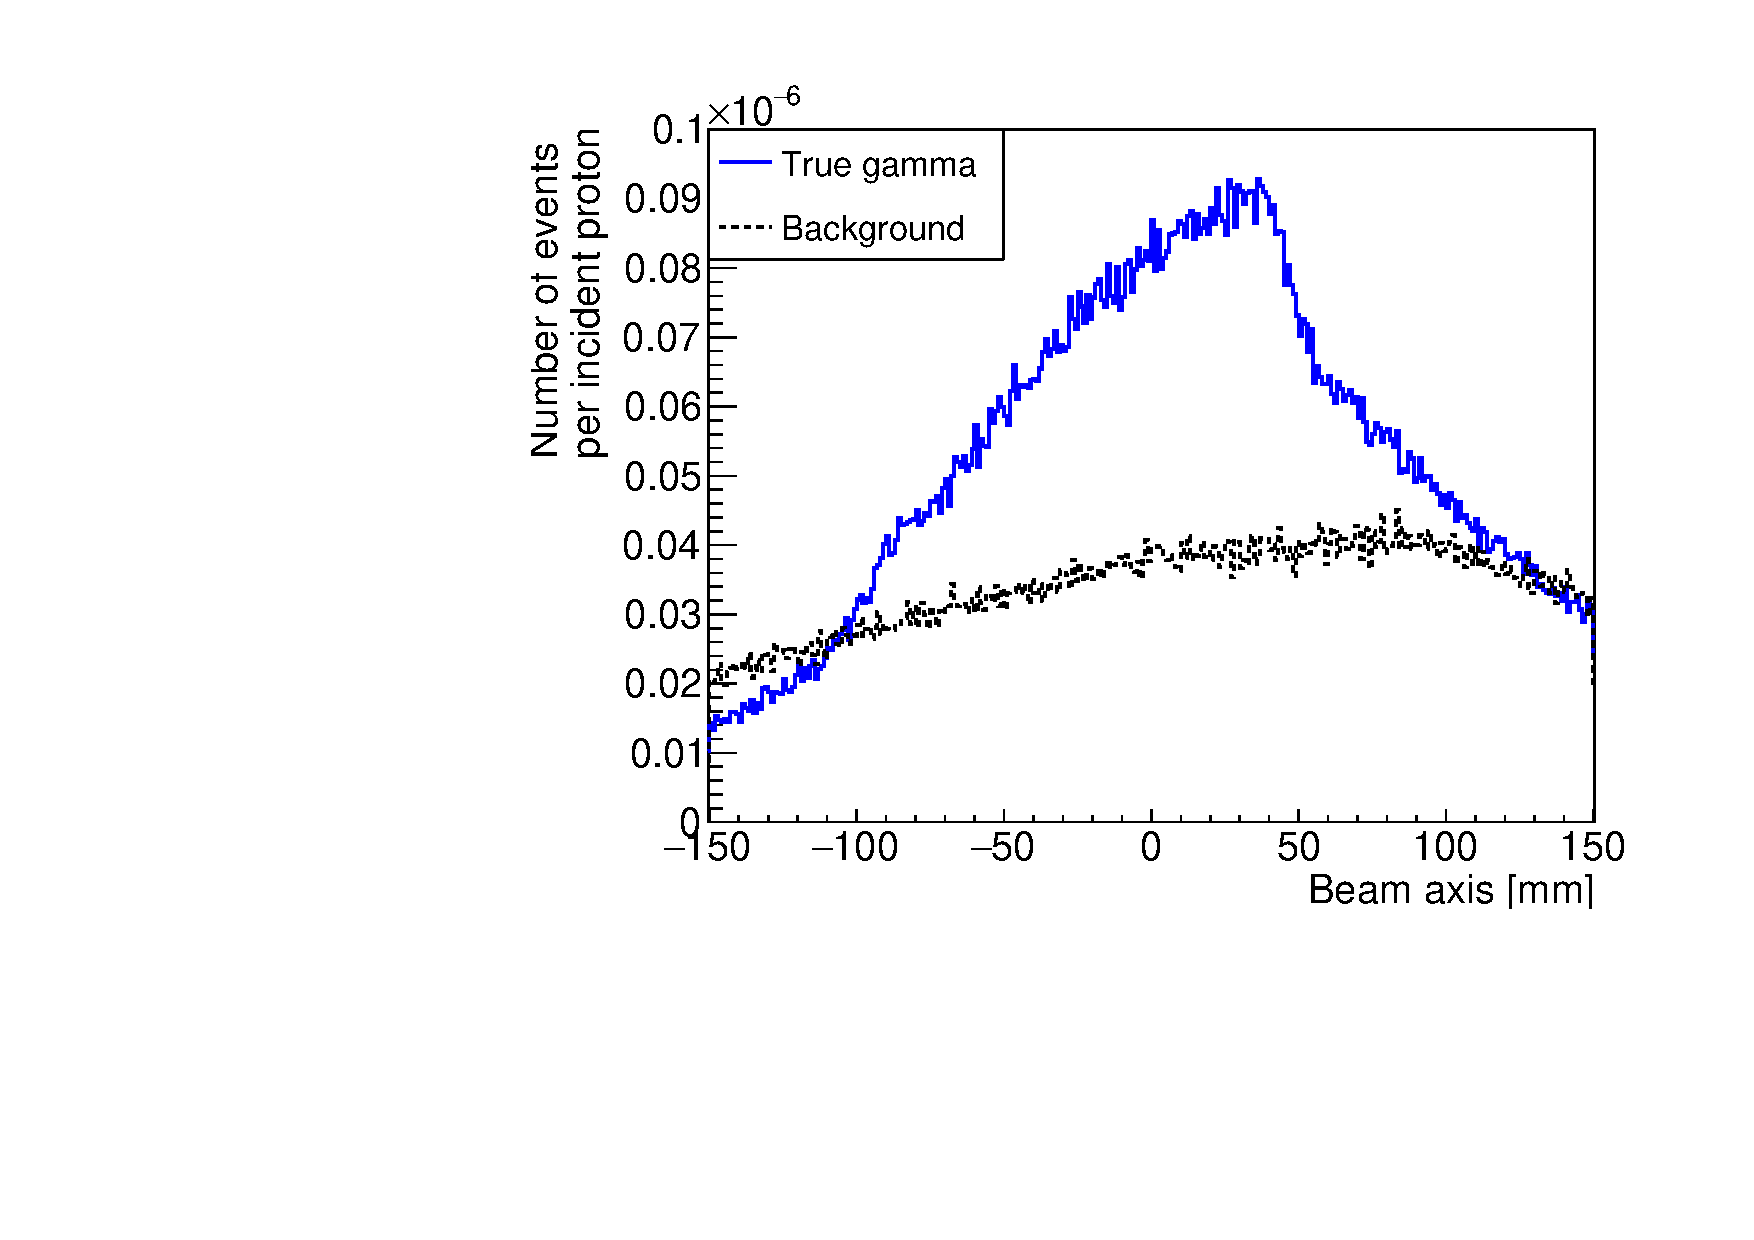
\includegraphics[width=0.48\textwidth]{./Figure/profile_high_stat_linecone_2.pdf}}
	\subfloat[\label{fig:fig_Results_Estimation_Camera_Profil_highStat_CC_simulation_Hadronth_LineCone}]{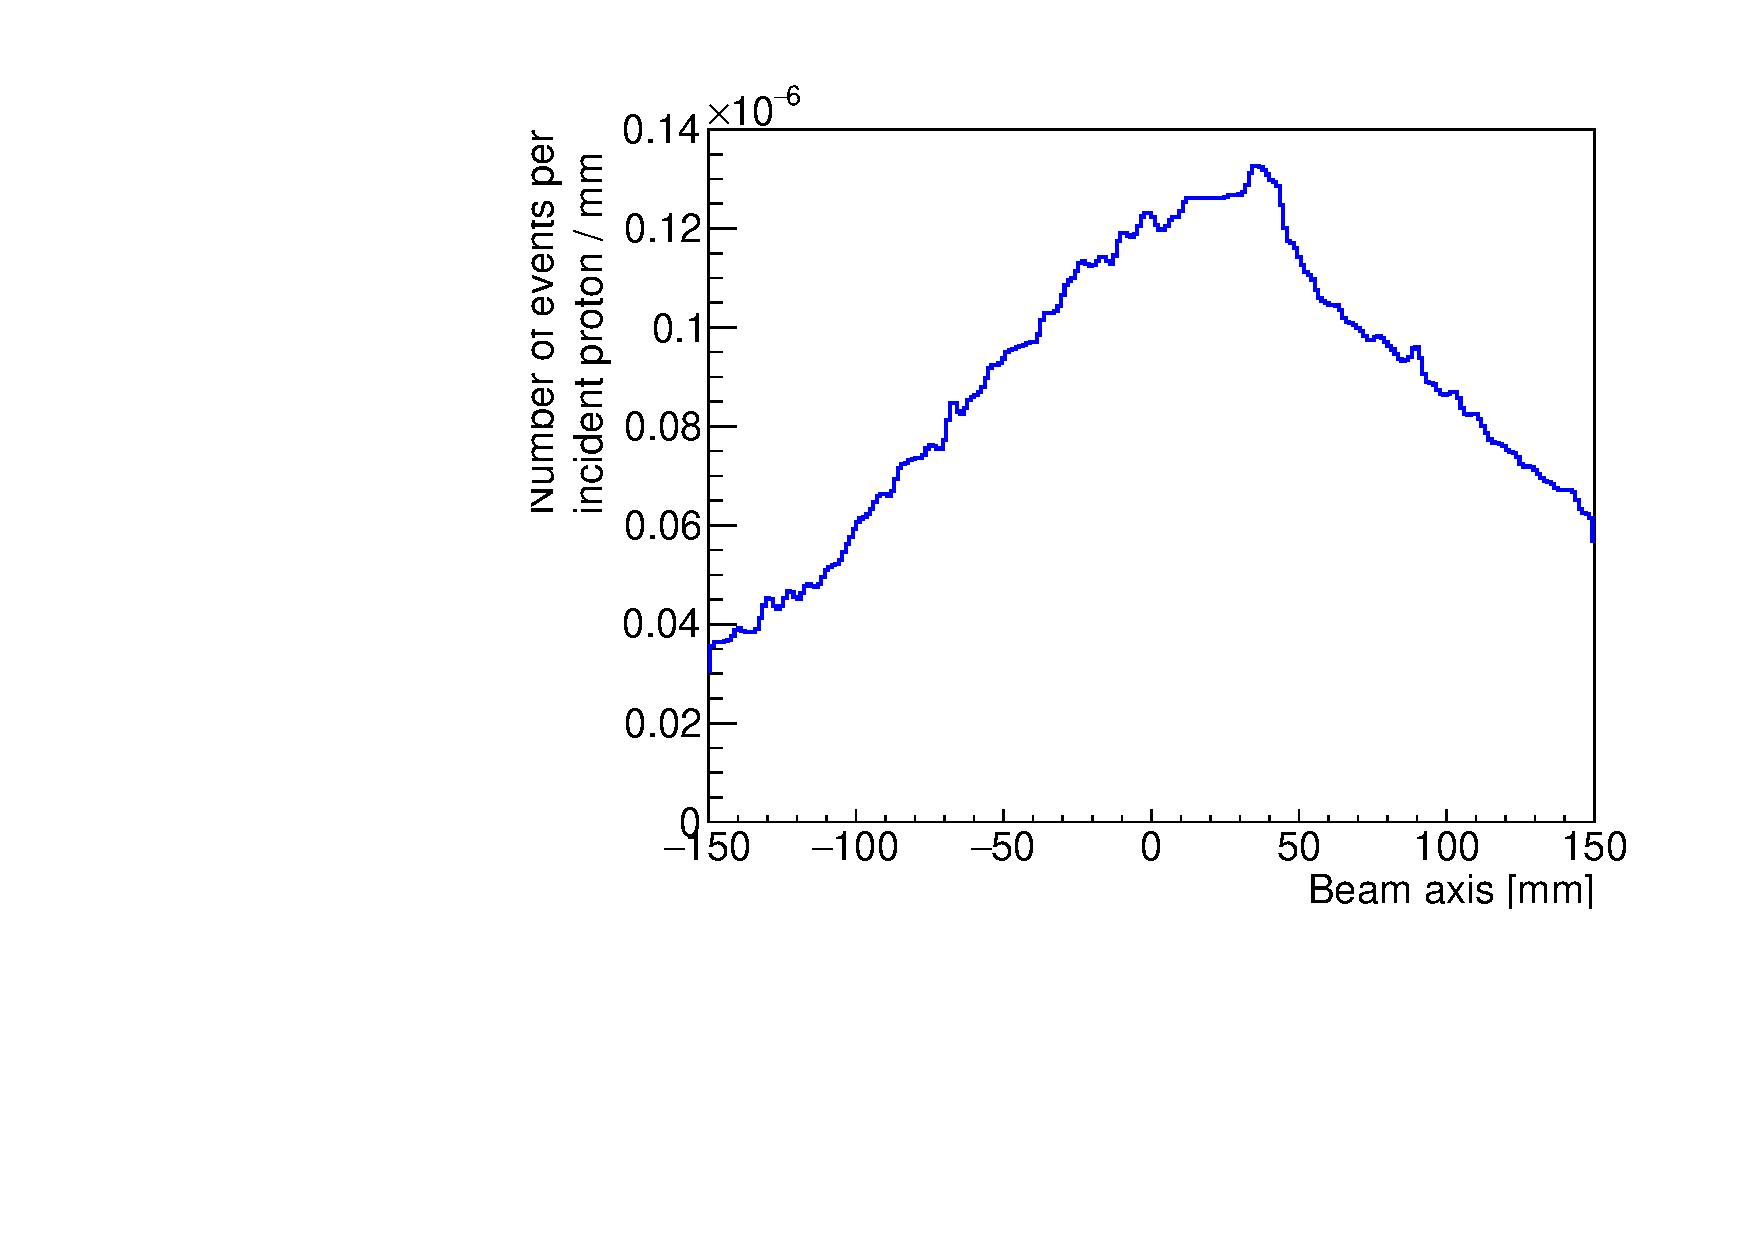
\includegraphics[width=0.48\textwidth]{03_GraphicFiles/chapter3/HT/new/reconstructed_histStat_profile_lineCone_norm.pdf}}
 % \subfloat[\label{fig:fig_Results_Estimation_Camera_Profil_highStat_CC_simulation_Hadronth_MLEM}]{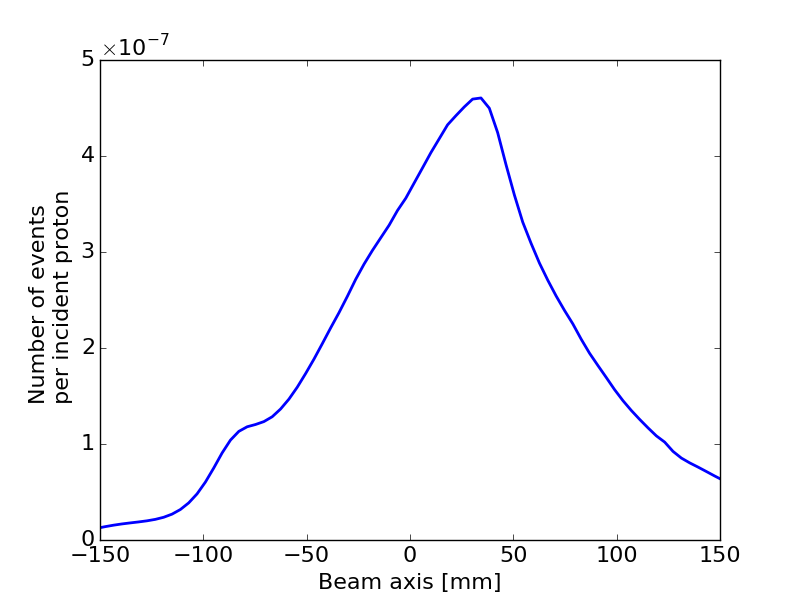
\includegraphics[width=0.48\textwidth]{./Figure/profileY_corr_r15.png}}\\
   \subfloat[\label{fig:fig_Results_Estimation_Camera_Profil_highStat_CC_simulation_Hadronth_MLEM}]{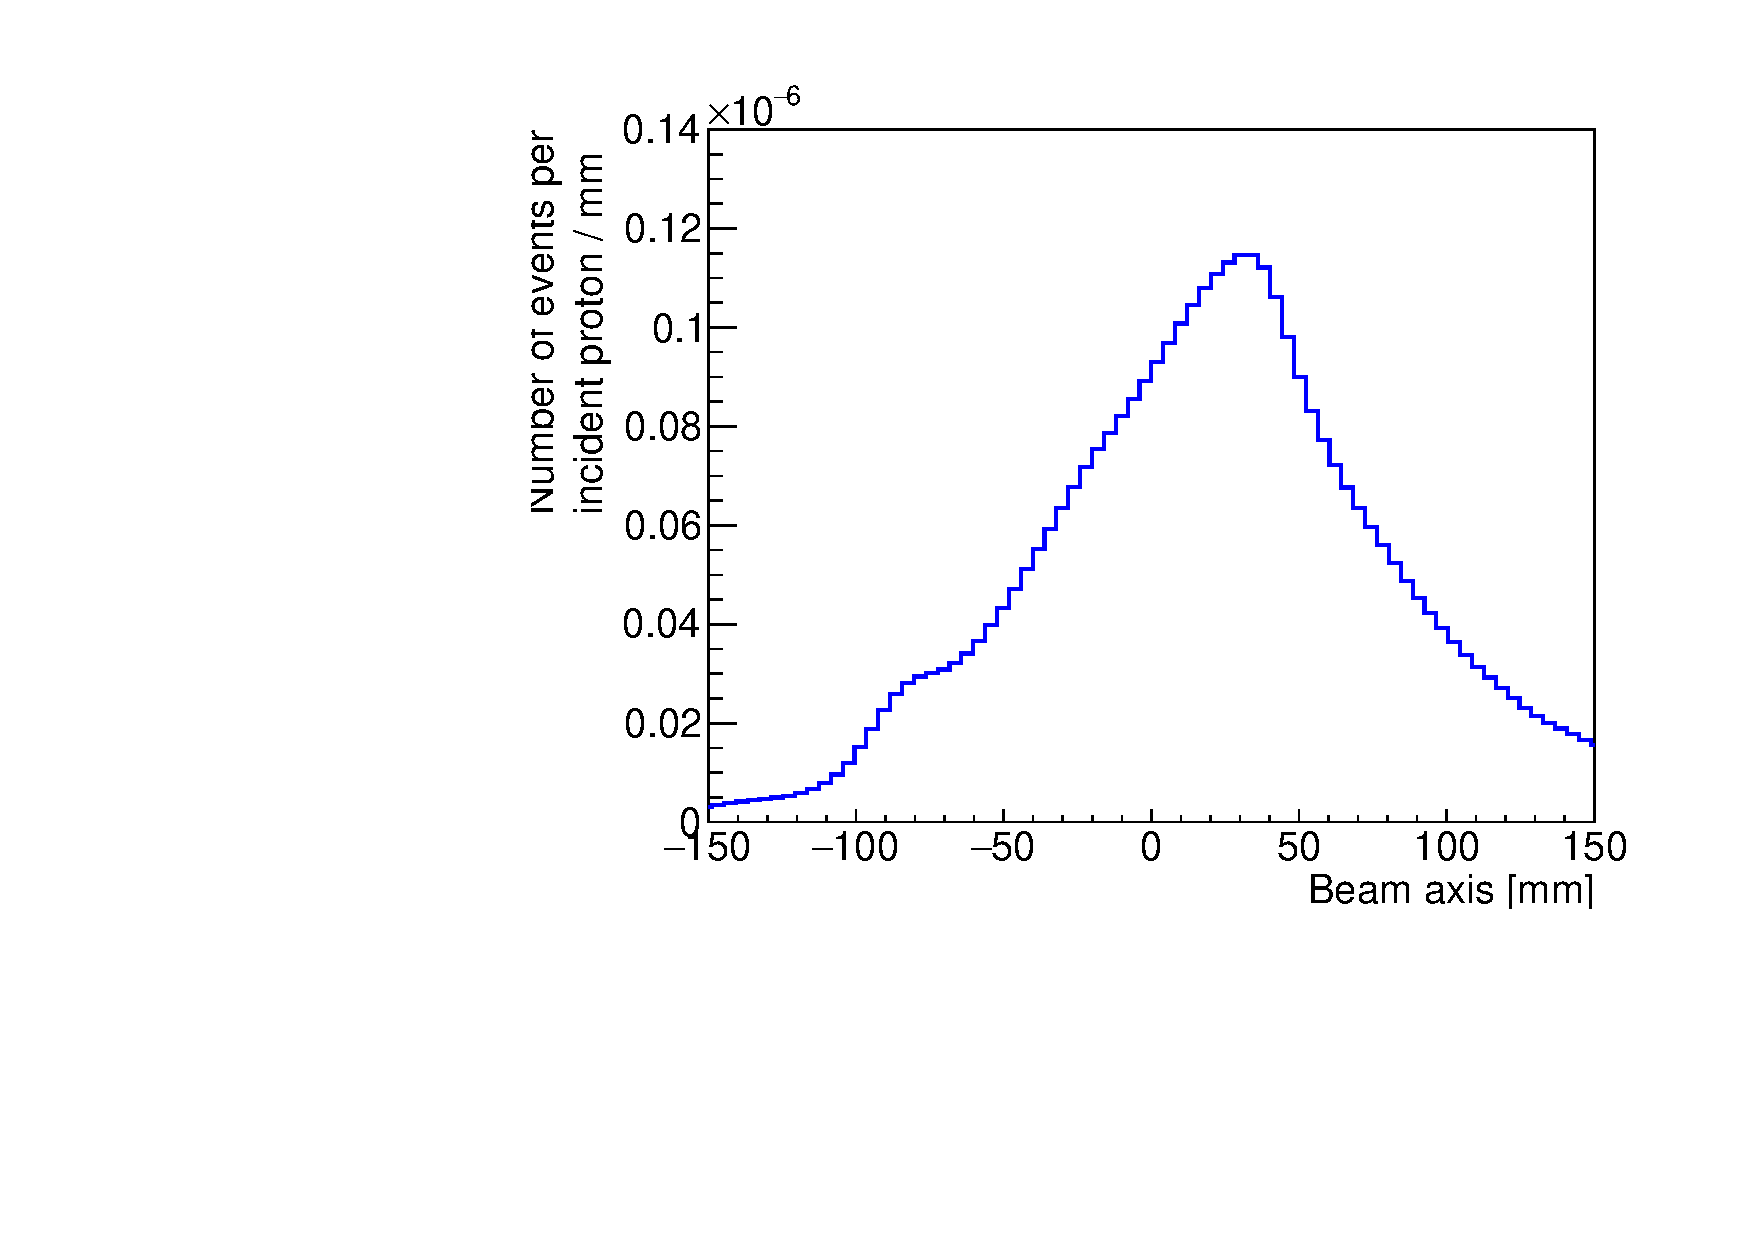
\includegraphics[width=0.48\textwidth]{03_GraphicFiles/chapter3/HT/new/reconstructed_histStat_profile_norm.pdf}}\\
  % \subfloat[\label{fig:fig_Estimation_Camera_CC_NURBS_Poisson_LC}]{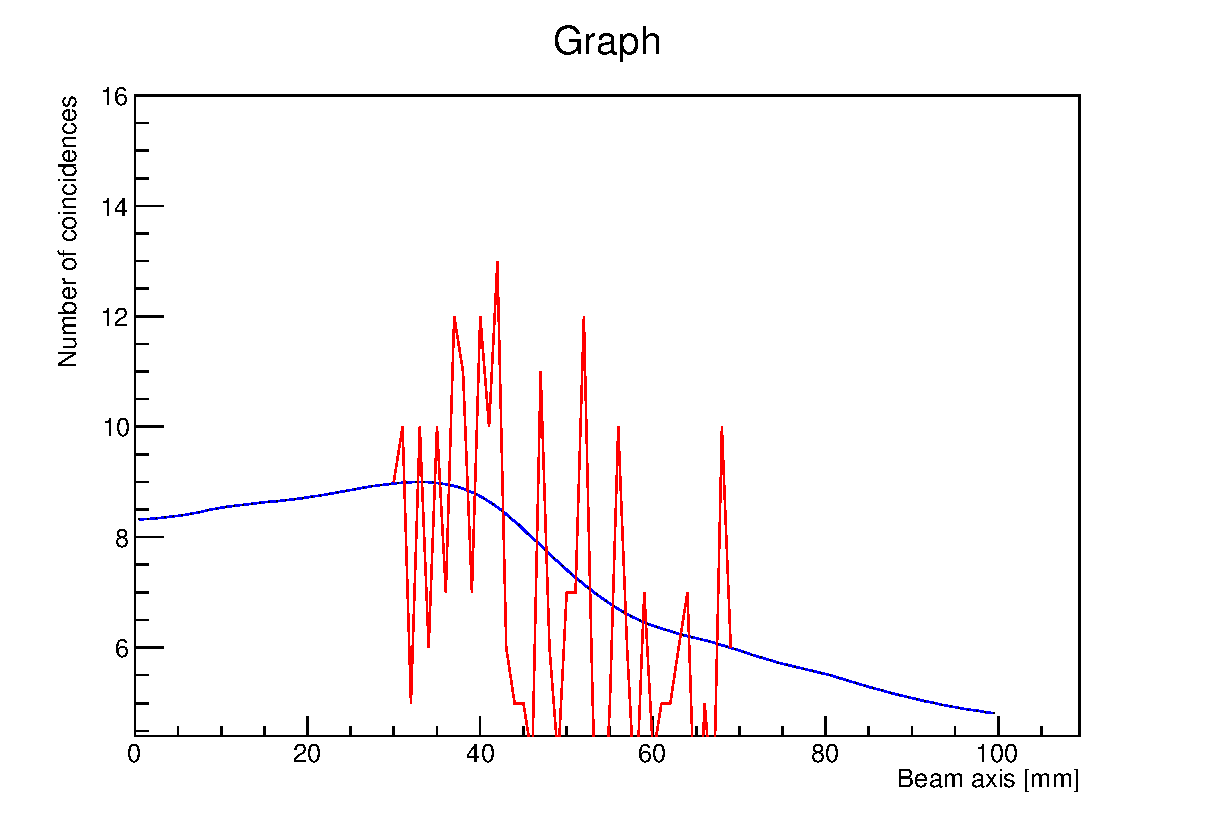
\includegraphics[width=0.33\textwidth]{./Figure/2017-08-02_Poisson_Nurbs_1e8_Article_LC.eps}}
  \subfloat[\label{fig:fig_Estimation_Camera_CC_NURBS_Poisson_LC}]{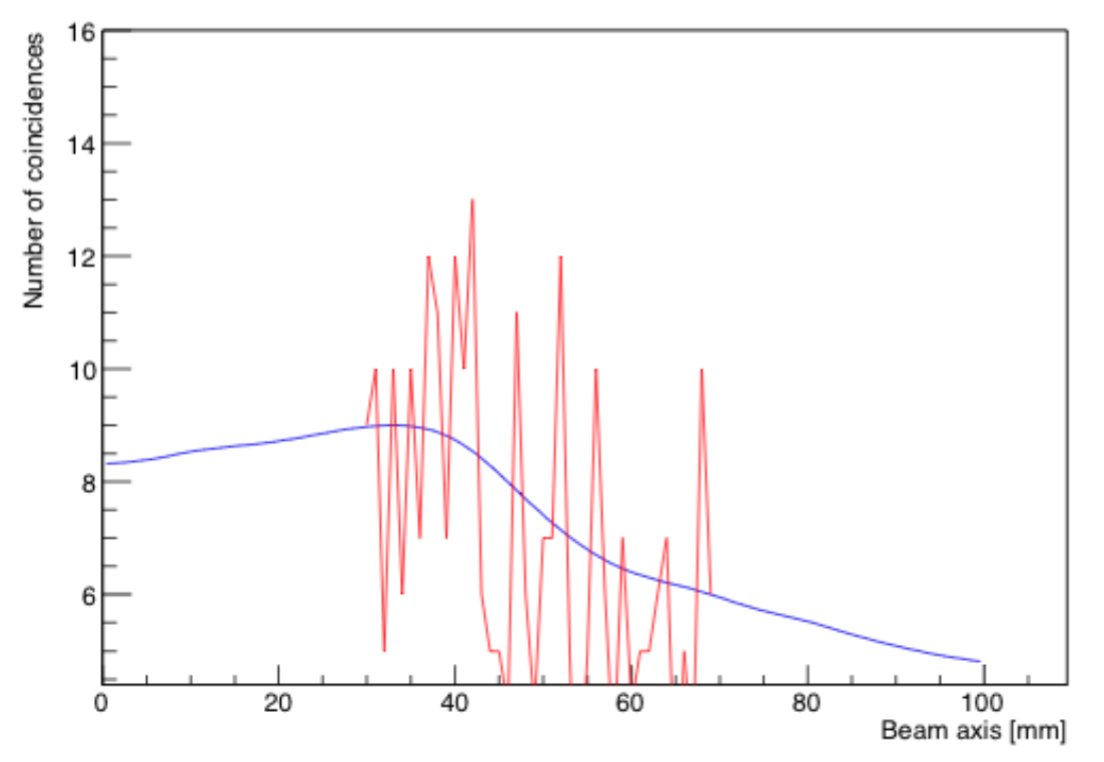
\includegraphics[width=0.48\textwidth]{./Figure/line_cone_NURBS.png}}
  % \subfloat[\label{fig:fig_Estimation_Camera_CC_NURBS_Poisson_MLEM}]{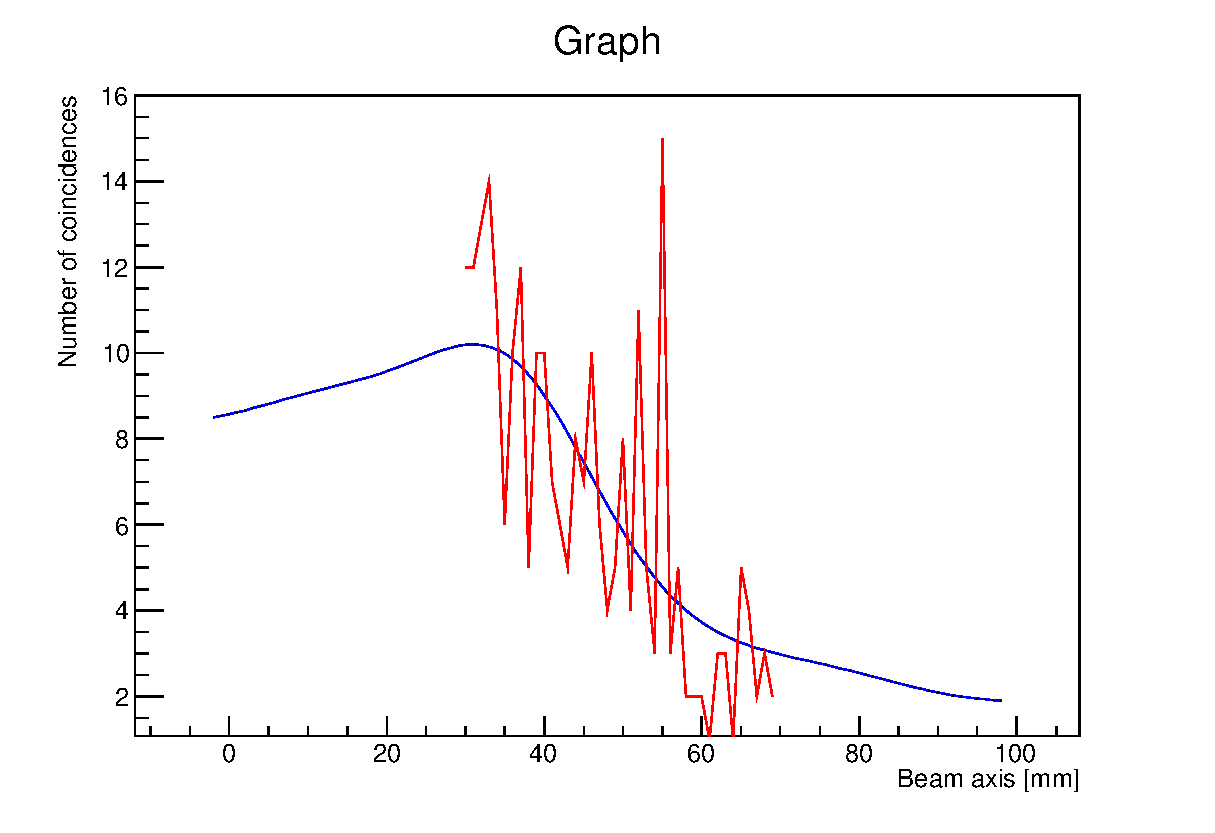
\includegraphics[width=0.33\textwidth]{./Figure/2017-08-02_Nurbs_Poisson_1e8_Article_MLEM.eps}}\\
  \subfloat[\label{fig:fig_Estimation_Camera_CC_NURBS_Poisson_MLEM}]{\includegraphics[width=0.48\textwidth]{03_GraphicFiles/chapter3/HT/MLEM_NURBS.png}}\\
  \caption{Data processing comparison for the same proton simulation with the line cone algorithm (left column) and the LM-MLEM algorithm (right column). The first row gives the reconstructed profile for $10^{10}$ incident protons. The second row shows the reference curve (blue) and the curve obtained with a $10^8$ incident protons subset.}% at the same statistics of $10^8$ incident protons.}
\end{figure}

\begin{figure}
  \centering
  % \subfloat[\label{fig:fig_Results_Chi2_Distribution_Variation_CC_simulation_Hadronth_LC}]{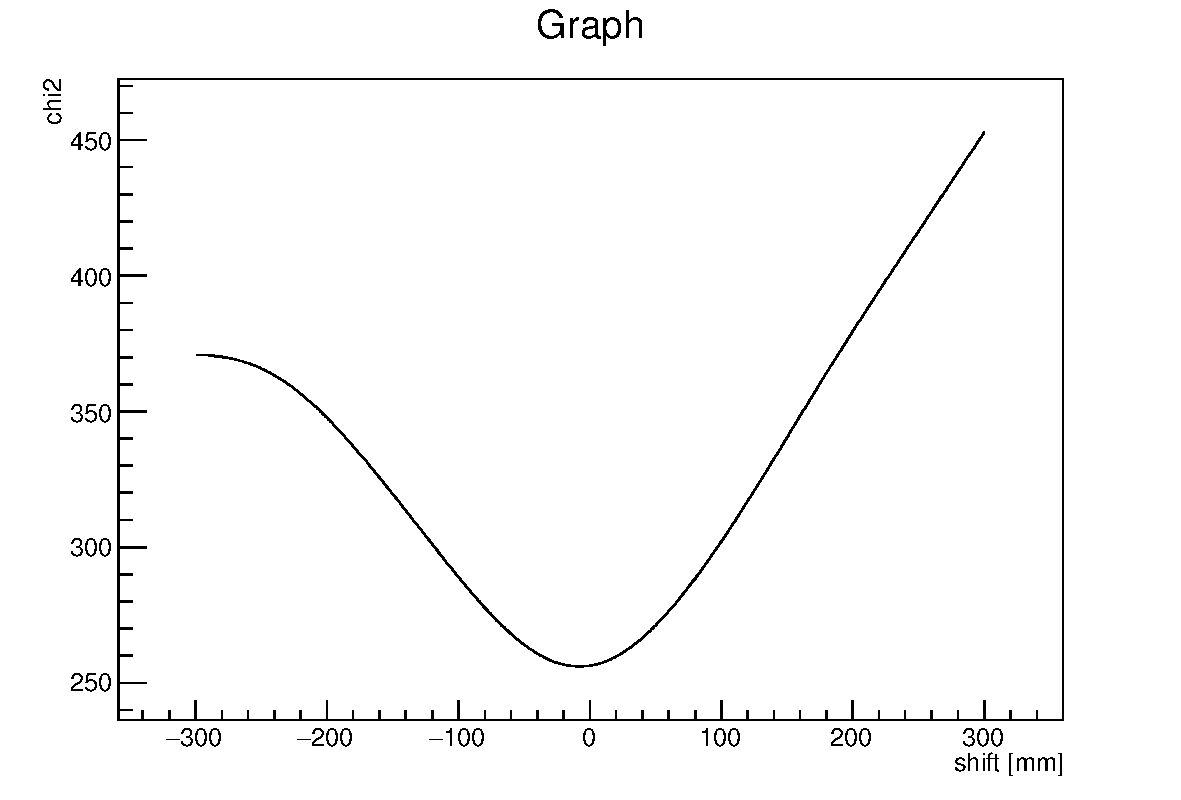
\includegraphics[width=0.33\textwidth]{./Figure/2017-08-02_Distribution_Chi2_1e8_LC.pdf}}
  \subfloat[\label{fig:fig_Results_Chi2_Distribution_Variation_CC_simulation_Hadronth_LC}]{\includegraphics[width=0.48\textwidth]{03_GraphicFiles/chapter3/HT/chi2_linecone.png}}
  % \subfloat[\label{fig:fig_Results_Chi2_Distribution_Variation_CC_simulation_Hadronth_MLEM}]{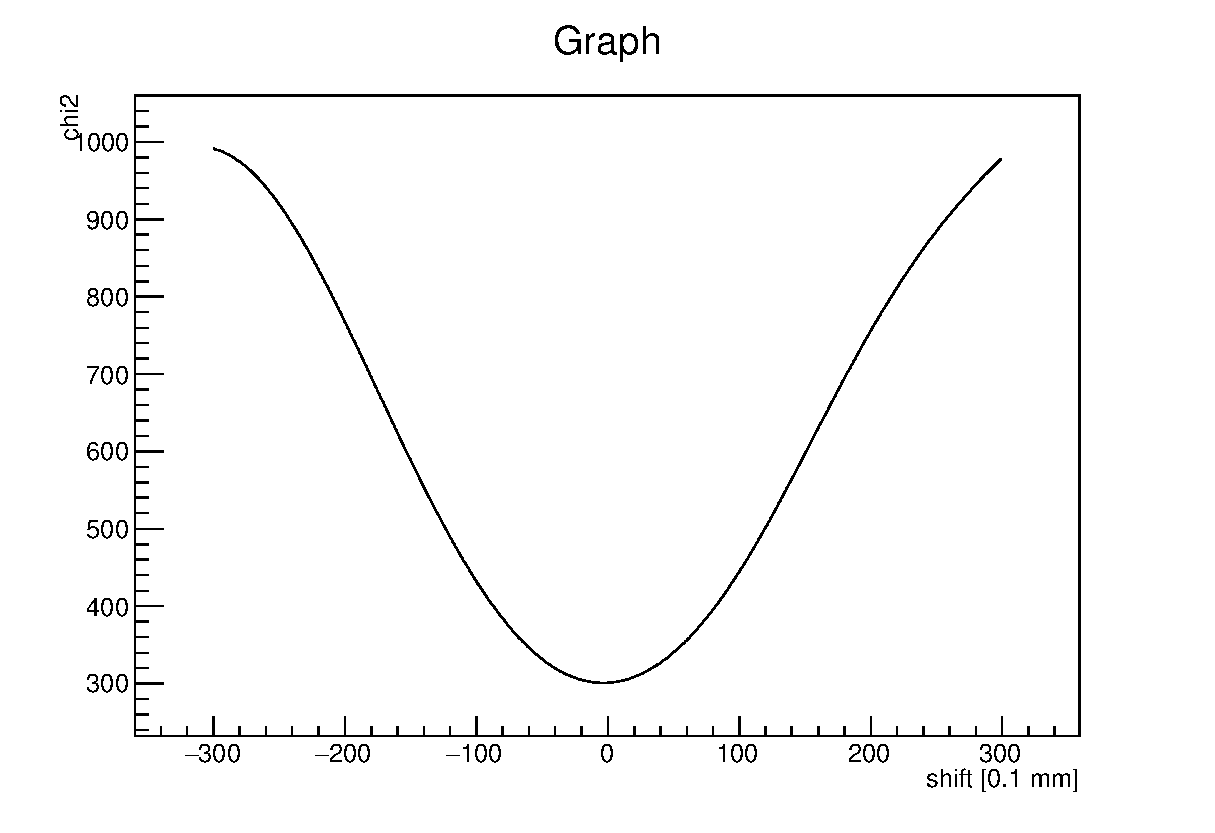
\includegraphics[width=0.33\textwidth]{./Figure/2017-08-02_Distribution_Chi2_Results_binning_1mm_ShiftNurbs0_1mm_1e8_article_MLEM.eps}}\\
  \subfloat[\label{fig:fig_Results_Chi2_Distribution_Variation_CC_simulation_Hadronth_MLEM}]{\includegraphics[width=0.48\textwidth]{03_GraphicFiles/chapter3/HT/chi2_MLEM.png}}\\
  % \subfloat[\label{fig:fig_Results_Precision_Distribution_Variation_CC_simulation_Hadronth_LC} ]{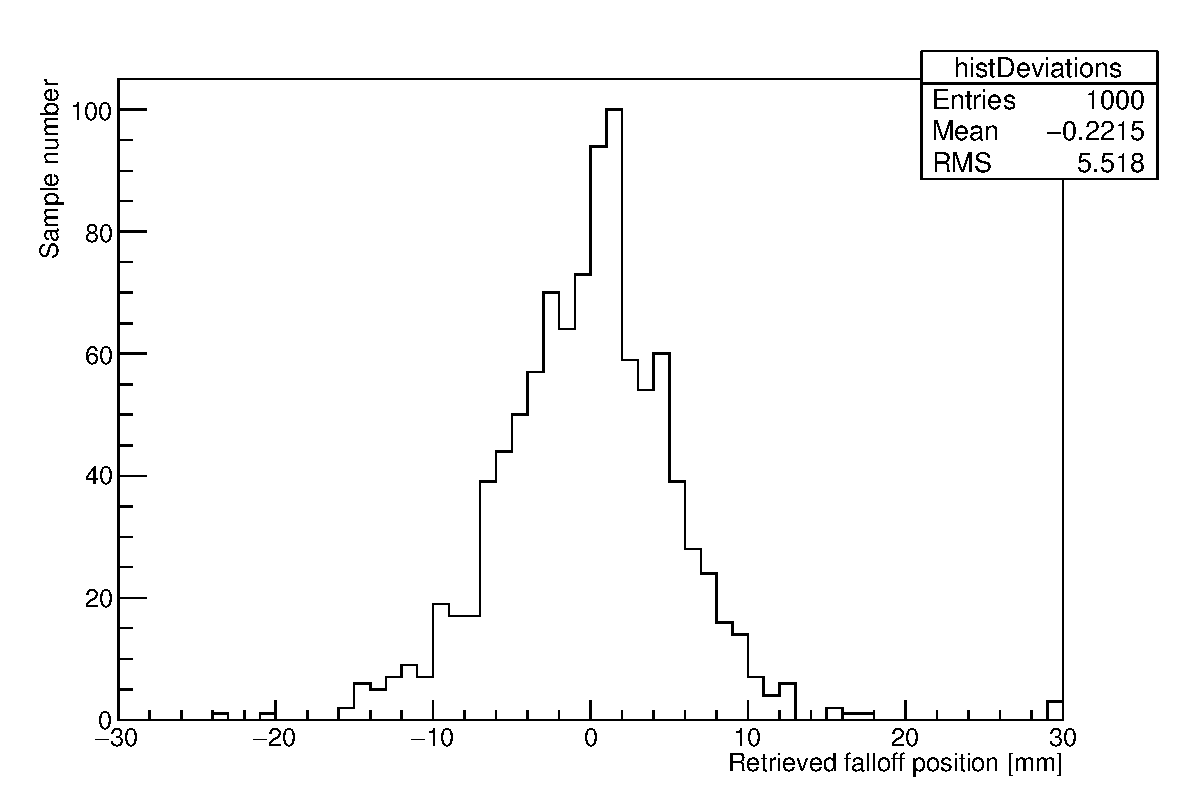
\includegraphics[width=0.33\textwidth]{./Figure/2017-08-02_Distribution_finale_1e8_Article_LC.pdf}}
  \subfloat[\label{fig:fig_Results_Precision_Distribution_Variation_CC_simulation_Hadronth_LC} ]{\includegraphics[width=0.48\textwidth]{03_GraphicFiles/chapter3/HT/deviation_linecone.png}}
  % \subfloat[\label{fig:fig_Results_Precision_Distribution_Variation_CC_simulation_Hadronth_MLEM} ]{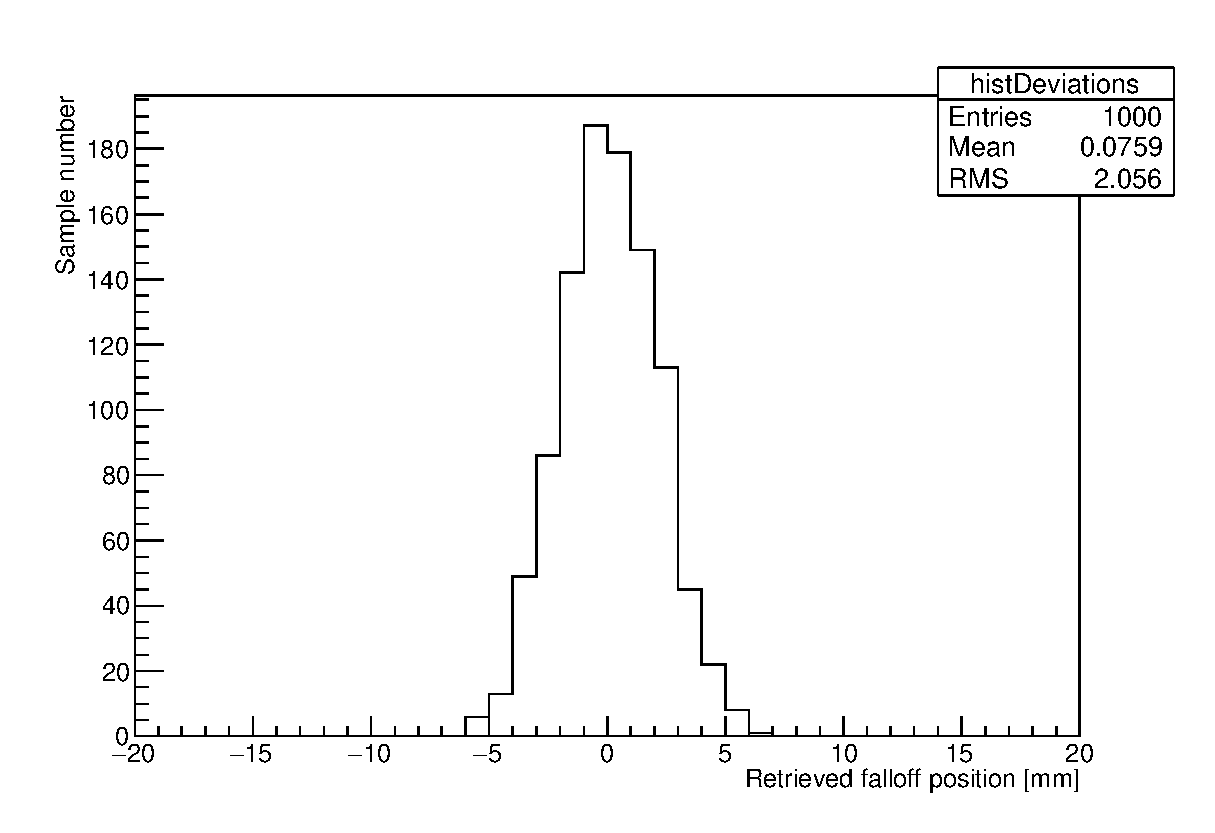
\includegraphics[width=0.33\textwidth]{./Figure/2017-08-02_FallOff_Results_binning_1mm_ShiftNurbs0_1mm_1e8_Article_MLEM.eps}}
  \subfloat[\label{fig:fig_Results_Precision_Distribution_Variation_CC_simulation_Hadronth_MLEM} ]{\includegraphics[width=0.48\textwidth]{03_GraphicFiles/chapter3/HT/deviation_MLEM.png}}
  \caption{Data processing comparison for the same proton simulation with the line cone algorithm (left column) and the LM-MLEM algorithm (right column). The first row shows the $\chi^2$ distribution for one data subset. The last row represents the distribution of the minimal calculated shifts for 1000 such subsets.}% at the same statistics of $10^8$ incident protons.}
\end{figure}

\begin{figure}
\centering
\subfloat[]{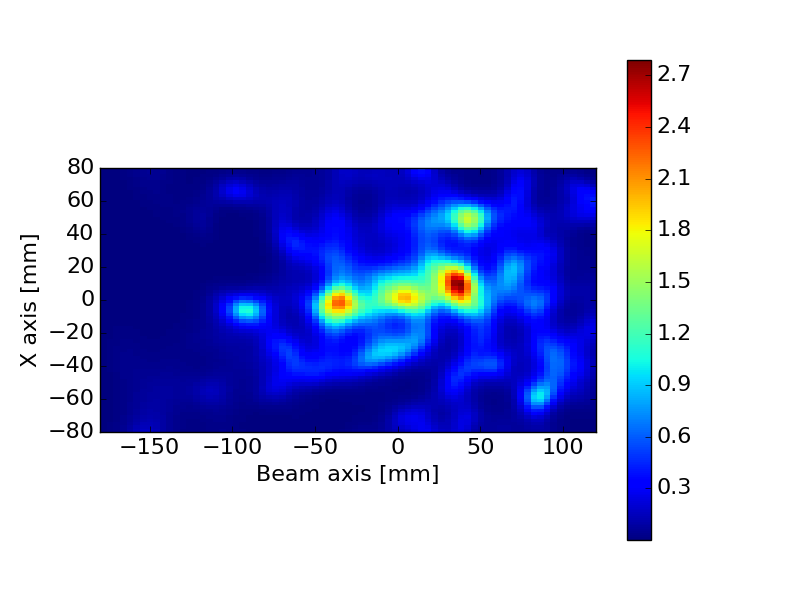
\includegraphics[width=0.5\textwidth,clip=true,trim=0 70 130 90]{03_GraphicFiles/chapter3/HT/projection2D_Z_corr_r20.png}}
%\subfloat[]{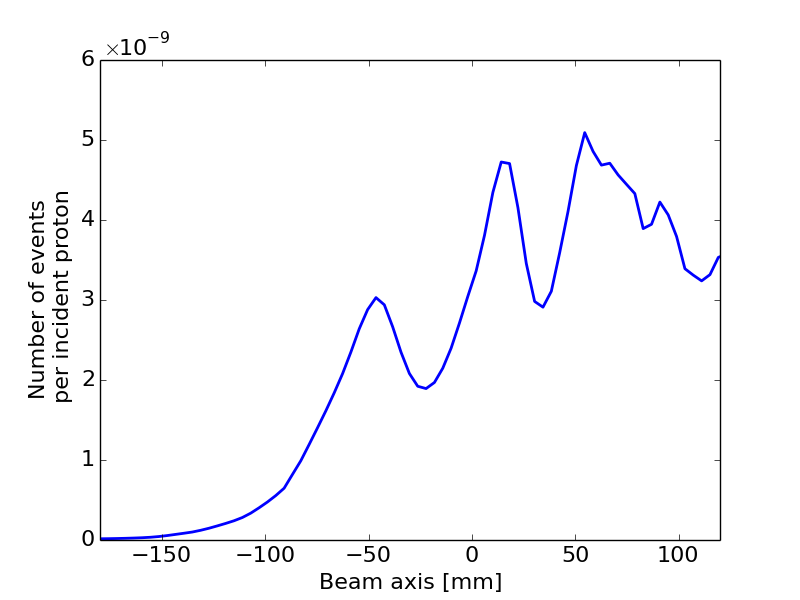
\includegraphics[width=0.5\textwidth]{./Figure/profileY_corr_r20.png}}\\
\subfloat[]{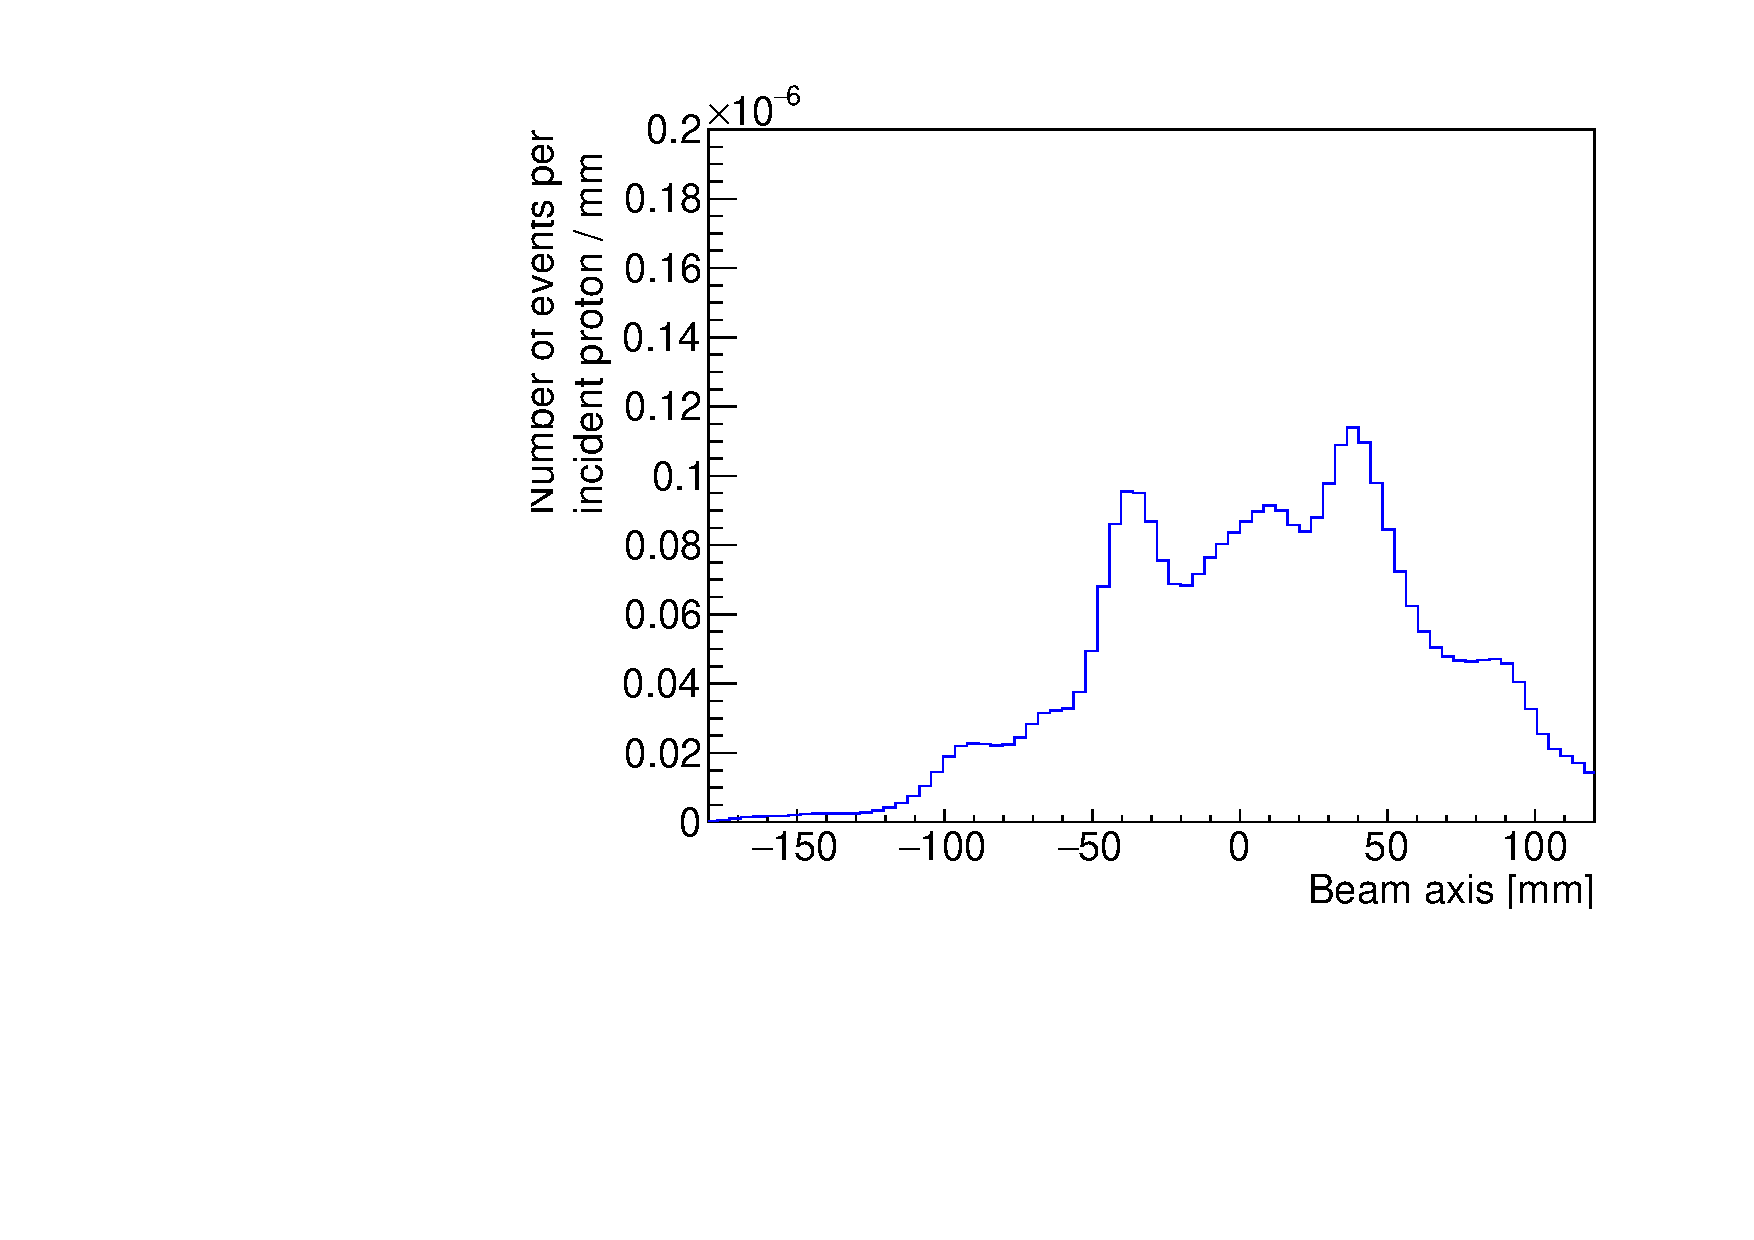
\includegraphics[width=0.5\textwidth]{03_GraphicFiles/chapter3/HT/new/reconstructed_lowStat_profile_norm.pdf}}\\
%\subfloat[]{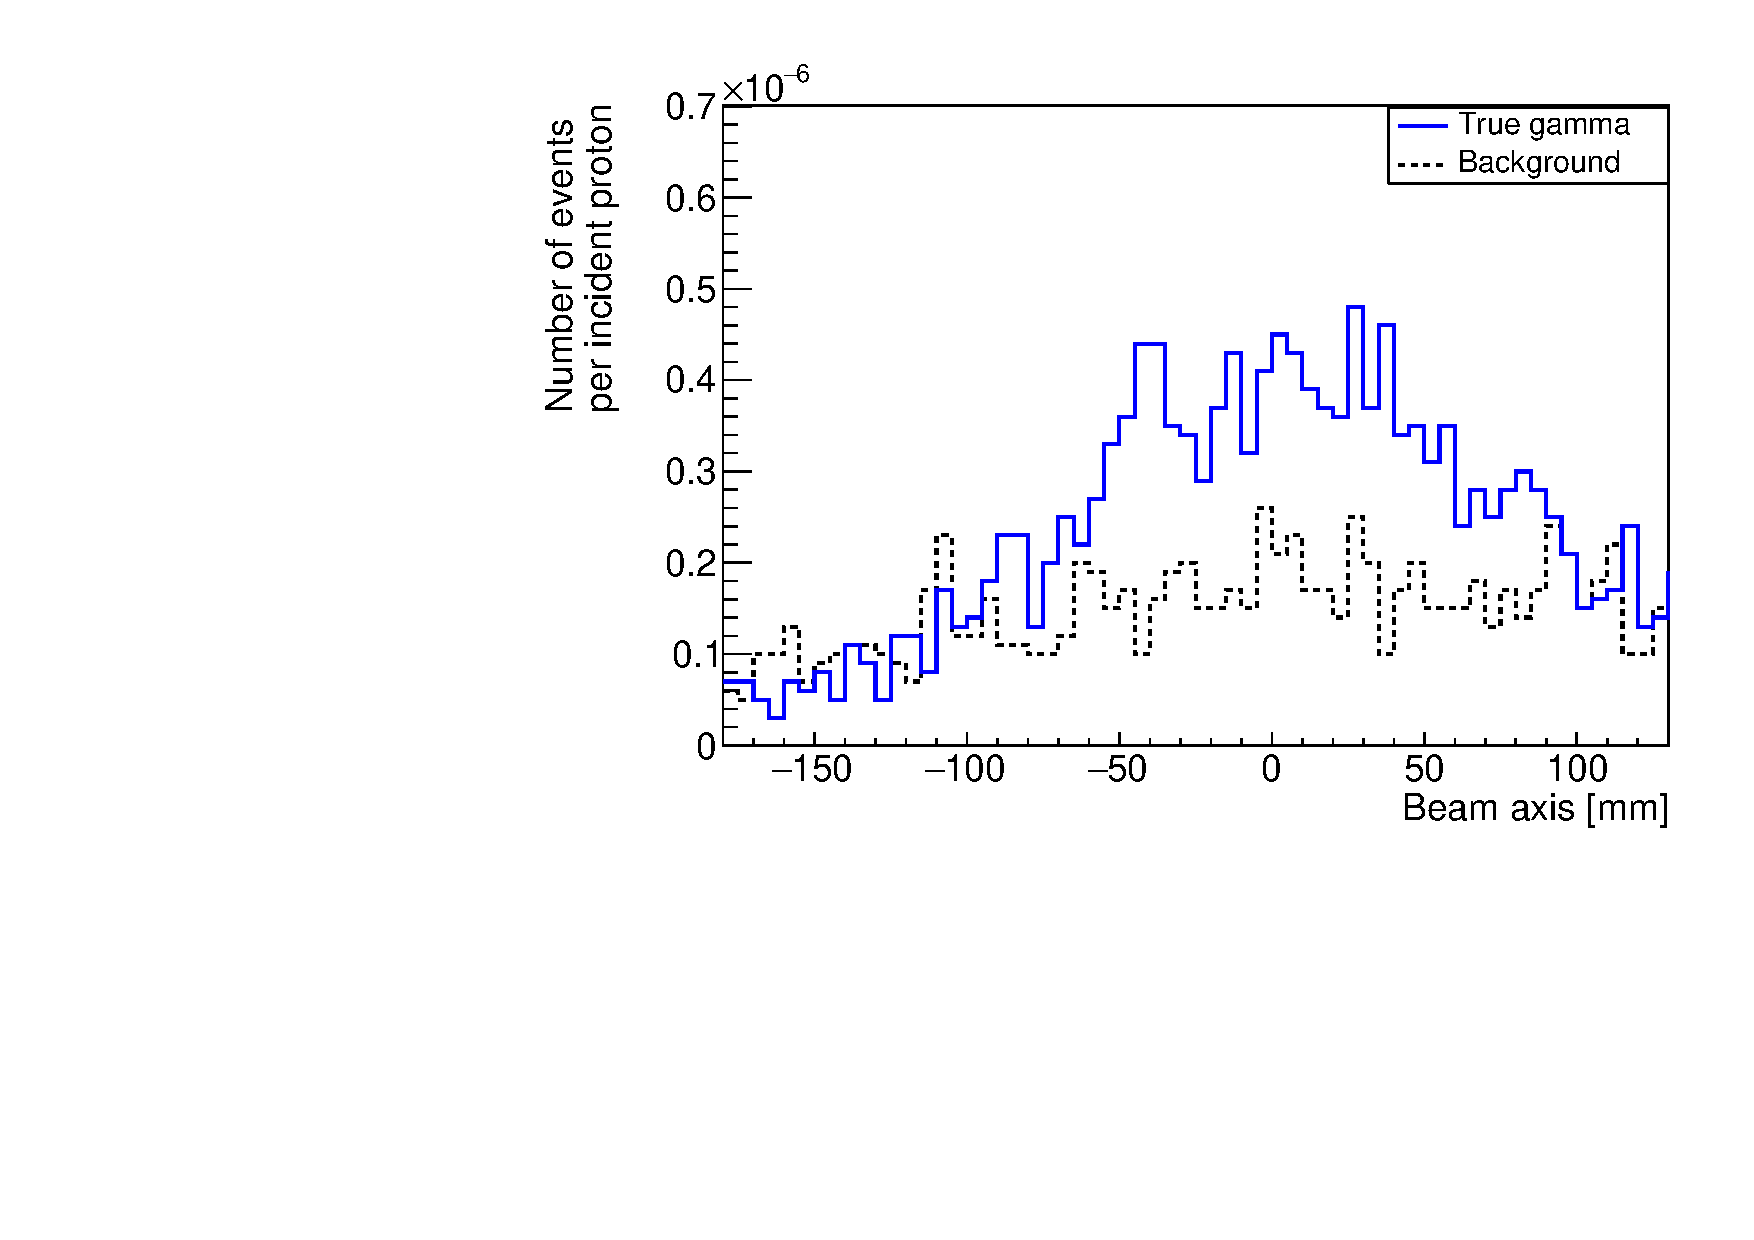
\includegraphics[width=0.5\textwidth]{./Figure/2015_02_16_Reconstruction_coinc_160MeVProton_TOF_6ns_file0to100_zoom.pdf}}
\subfloat[]{\includegraphics[width=0.5\textwidth]{03_GraphicFiles/chapter3/HT/new/recon_profile_line-cone_lowStat_norm.pdf}}

\caption{Line-cone and LM-MLEM reconstruction for a 160~MeV proton beam, $10^{8}$ total incident protons. The beam intensity is 1 proton per bunch. The Compton camera is centered at the expected Bragg peak position, $y=+50\,$mm. The time-of-flight event selection is applied on the collected data set. 20 iterations are performed for the MLEM reconstruction.
Figure (a) represents the MLEM reconstructed 2D image in the plane $(x,y)$, parallel to the camera entrance surface. The position $x=0\,$mm corresponds to the center of the PMMA phantom and the $y$ direction corresponds to the beam axis, with the target entrance at $y=-100\,$mm and the target end at $y=+100\,$mm.  In figure (b) the 1D profile along the $y$ axis is sketched. The profile fall-off is located at $y=+50\,$mm. Figure (c) shows the profile obtained by means of the line-cone algorithm for the same time-of-flight selected data.}
\label{fig:comparison}
\end{figure}


The analysis method described in section~\ref{MatMeth:precision} is applied to the different PG obtained profiles to retrieve the camera precision in the falloff identification. The results are shown in figure~\ref{fig:precision}, where the two reconstruction methods are represented by different markers.

\begin{figure}	
\centering
\includegraphics[width=0.7\textwidth]{03_GraphicFiles/chapter3/HT/2017-10-21_Precision_Comparaison_linecone_MLEM_Article_Fit.eps}
\caption{Fall-off retrieval precision (FRP) for two different reconstruction algorithms: line-cone and LM-MLEM. The precision is shown as a function of the total number of incident protons, in the range $1\times10^{8}$ to $5\times10^{9}$.}	
\label{fig:precision}
\end{figure}

The iterative MLEM reconstruction method enables one to achieve a better precision, with a reduction of about 3~mm of the falloff retrieval accuracy in the whole range of statistics explored. A linear behavior, highlighted by the performed linear fit of the two data sets, is verified with increasing number of primary protons, starting from the single spot scale of about 10$^8$ primaries, till $5\times10^9$ protons, which can correspond to the monitoring of a group of spot with the same planned range. 

\section{Discussion}

We studied in this simulation work the performance of the CLaRyS Compton camera prototype and its possible implementation as prompt gamma detector for ion beam therapy monitoring. The proposed analysis is focused on three main points: absolute gamma detection efficiency, true and random coincidence rate and camera precision in the identification of the prompt gamma emission profile fall-off.

The absolute gamma detection efficiency has been measured with the detector exposed to gamma sources at six different energies, and the efficiency variation as a function of the source position has been reported. The whole study has been performed with a fixed camera geometry, but different geometrical configuration can change the obtained results. In~\cite{Fontana_APPB} we tested the same prototype with two absorber configurations, showing an absolute efficiency reduction of a factor approximately two when reducing the absorber from a $8\times6$ block matrix to a $3\times3$ one. To this efficiency reduction corresponds an increased spatial resolution, probably given by the selection of gamma scattered with small angles. This hypothesis is confirmed by the efficiency variation generated by the applied energy thresholds. Indeed, for low energies, below 2~MeV, the increased efficiency in the central section of the camera active surface shown in figure~\ref{fig::efficiency_study}(a) is linked to the increased relative number of photons approaching the camera with small angles. These photons are more likely undergoing Compton scattering with a reduced energy deposition, which is recorded by an ideal detector and rejected by the energy threshold. The effect is all the more important as the primary gamma energy is limited, creating the peculiar energy dependence of the efficiency reduction observed in the results in figure~\ref{fig::efficiency_study}(b). Therefore, in case the compactness of the detector must be privileged, the efficiency reduction is not dramatic for the Bragg peak monitoring purpose. Moreover, such a compact configuration allows for the implementation of several detector heads, which can be set at different angles and provide additional spatial information. In case the highest possible efficiency is required, the distance between scatterer and absorber can be modified, knowing that for reduced distances the efficiency is increased because a minimal amount of scattered photons escapes the absorber field of view. On the other hand, a reduction of the inter-detector distance is not recommended for accurate TOF measurements (for fixed target-scatterer distance), given the uncertainty added by the detectors time resolutions. In addition to this, also the spatial resolution is affected by a reduction of the scatterer-absorber distance, given the increased amount of photons scattered with large Compton angles included in the collected events. Indeed, large angle scatterings tend to degrade the spatial resolution.   
Regarding the dependence of the efficiency on the Compton camera position, an accurate setup with respect to the expected Bragg peak position appears mandatory for the detection optimization.

A further study showed how this effect is mainly due to the cut applied on the scatterer detector. 
%The results emerged from the analysis of the rate of true and random coincidences with respect to the beam intensity show how at a realistic clinical intensity the signal-over-noise ratio is very low (less than 0.1) for both raw and reconstructed events and for proton and carbon beams. 
The study of the signal to noise ratio as a function of beam intensity was performed (see figure \ref{fig:coincidences}). The results show that, at clinical intensities, this ratio is very low. The TOF selection is effective in the case of carbon beams, where a significant proton and neutron contamination is expected. If we consider the case of proton beams, the amount of random and true coincidences is comparable at an intensity of about 1 proton per bunch, so that a clinical intensity reduction should be necessary to fit this configuration. Even if a possible image reconstruction is not excluded by the low signal-over-noise ratio detected at realistic beam intensity, given the fact that the random coincidence are distributed in an homogeneous way in the reconstructed volume, an intensity reduction can be an option in order to obtain more significant data sets. It must be noticed that the need for Bragg peak position online check is all the more necessary for distal spots, which are in general the first to be treated, so that a beam intensity reduction at the beginning of the treatment can be foreseen in case an accurate monitoring is strictly needed. This would not affect the treatment delivery, nor the planned patient rate in the clinical work-flow. 
In the case of carbon ions, the larger amount of secondary neutron produced during the patient treatment seems to require other background rejection methods in order to lead to an advantageous signal-over-background ratio. Note also that online filtering strategies  may be used to improve the quality of the date: already in figure \ref{fig:coincidences}, one can notice that the amount of reconstructed events is about half that of true gamma, which means that partial absorption in the absorber leads to events which cannot be reconstructed via the line-cone method. More refined pre-analysis could be used and have been proposed in \cite{Draeger:2017aa}.

The camera precision has been estimated starting from a reference prompt gamma emission profile obtained at high primary particle statistics ($10^{10}$), with the random extraction of 1000 data subsets per intensity and applying a minimization robust algorithm to define the shift of the identified profile fall-off with respect to the reference one.
The camera precision in the falloff identification rapidly increases for increasing primary particle statistics. A sufficiently good precision is achieved on a spot basis for proton beams, where the precision is about 2~mm with a MLEM reconstruction: a qualitative monitoring of each spot seems then possible. In order to achieve millimeter or sub-millimeter precision, some spot grouping methods must be considered. As a general result, the LM-MLEM iterative algorithm, which is now the standard for this kind of image reconstruction,  guarantees a better fall-off identification precision over the whole explored intensity range. However, MLEM does not exploit the additional information provided by the knowledge of the beam position in the transverse plane. In future studies, such a priori information should be considered in order to improve the reconstruction rapidity and image quality. At present, given the long calculation time required by the iterative algorithm, the line-cone reconstruction method can still be an option for on-line treatment check, when safety limit can be fixed in order to exclude severe deviation from the treatment planning and an interruption of the dose delivery in real time can be foreseen. Moreover, the TOF information can be included in the line-cone reconstruction method in order to constrain the emission on a single point, and improve its accuracy.

The Compton detection principle has already proven its potential in detecting prompt gammas for ion beam therapy monitoring purpose, and the CLaRyS Compton camera prototype shows promising results for this application. The detector is now at the final development stage, its components are being tested on beam in clinical facilities and a first beam test with a complete system is foreseen for the next year. New simulation studies are to ba carried out to benchmark the Compton camera device to other detection systems, like PET machines or collimated detectors, already used or tested in clinics for ion beam therapy monitoring.            



\clearpage
%\printbibliography[heading=subbibintoc]


\chapter{Compton camera application in nuclear medicine}

\vfill

\minitoc

\newpage


\section{Introduction}\label{intro}
Single Photon Emission Computed Tomography (SPECT) is one of the most widespread techniques for nuclear medicine diagnostics examinations. In most of the clinical cases, a radiotracer is injected in the patient and the emitted $\gamma$-rays are collected by scintillating detectors coupled to physical collimation systems. This process leads to the reconstruction of a planar transmission image. Such a kind of imaging tool relies on the first idea proposed by Hal Anger~\parencite{Anger1958, Anger1964}, and it is now commercially available in different variants with peculiar features and applications. A complete system is often composed of at least two rotating detection heads, allowing a tomographic data acquisition and the reconstruction of a three-dimensional image of the radiotracer distribution.

The main consequence of the collimation system is a forced trade-off between sensitivity and spatial resolution: The spatial resolution is completely determined by the collimator geometry, and it can only be increased by reducing the collimator hole size, at the expense of a reduction in the detector sensitivity since fewer photons survive the mechanical selection. Moreover, the collimator thickness and septa limit the primary energy acceptance, and the performance of Anger cameras generally downgrades as energy increases. %mod ref 1   

In order to overcome this mechanical collimator limitation, it is natural to move towards an \enquote{electronic collimation}, where the emitted photons are tracked and the emission point is reconstructed via Compton kinematics. Compton cameras have been originally designed for astronomy applications (in particular for two-dimensional imaging of distant gamma sources), but the translation to the medical imaging and diagnostics is straightforward~\cite{Everett, Singh_CC}, in particular for what concerns the application in SPECT.

A Compton camera is generally composed of two kinds of detectors: a scatterer, ideally including one or more position sensitive detector, possibly thin and of low-$Z$ material, mainly to maximize the probability of Compton interaction with respect to photoelectric absorption; an absorber, generally configured as a segmented block of scintillating high-$Z$ material, in order to have the highest probability of complete photon absorption by photoelectric effect (even after multiple interactions). Events of interest correspond to photons that first interact with the scatterer transferring part of their energy to an electron, and then travel with reduced energy until the final absorption in the high-$Z$ detector. Such events can be selected based on time coincidences. The possible emission point is reconstructed and limited to the surface of a cone  with a half-opening angle \(\theta\). Its vertex is the Compton interaction point detected in the scatterer section. \(\theta\) is the Compton scattering angle and can be computed thanks to the Compton scattering relation~\cite{Compton1923} in equation~\ref{Compton_formula}:\\
\begin{equation}
\cos\theta\,=\,1-\frac{m_{e}c^{2}E_{1}}{E_{2}(E_{1}+E_{2})},
\label{Compton_formula}
\end{equation} 
where \(m_{e}c^{2} = 511\)~keV, \(E_{1}\) and \(E_{2}\) are the energies, respectively, deposited in the scatterer and the absorber. This formula assumes that the provided \(E_{1}\) corresponds to the full energy of the scattered electron. In cases when Compton electrons deposit only part of their energy in the scatterer detectors, the reconstructed angle is underestimated.

In the case of nuclear medicine applications the initial photon energy \(E_{0}\) is known and the complete photon absorption is not necessarily required thanks to the relation \(E_{0} = E_{1}+E_{2}\). 

The interception of several cone surfaces allows one to obtain the radiotracer distribution in two dimensions (or even three dimensions~\cite{McKisson3D}) with a single compact detector. Equation~\ref{Compton_formula} represents the ideal case, while in reality the Compton cone reconstruction is affected by the so-called Doppler broadening~\cite{Doppler}. The initial momentum of the Compton recoil electron (bound initial state) is not known and not included in the formula, generating a blur in the Compton reconstructed angle associated to the same incident energy. This effect is all the more reduced with low-$Z$ scatterer material.

L. Han and colleagues~\cite{HanComp} have performed a simulation work comparing a standard Anger camera and a Compton camera prototype for a fixed source energy of 364~keV (iodine-131 gamma ray emission). The expected enhanced detection efficiency associated to the Compton camera with respect to the Anger system was estimated to a factor 20 at the tested energy, while the spatial resolution was compared for equal imaging time. 

The aim of the present work consists in extending the aforementioned study to a wide energy range, with simplified analysis methods. The two systems under consideration are the Infinia Anger camera delivered by General Electrics Healthcare~\cite{AC_datasheet} and the Compton camera prototype under development by a collaboration of five laboratories in France~\cite{Krimmer2015} (CLaRyS - Contr\^{o}le en Ligne de l'hadronth\'{e}rapie par Rayonnements Secondaires) that consists of silicon detectors (scatterer) and bismuth germanium oxide (BGO) blocks (absorber). The detector performances are compared in terms of efficiency and spatial response with the exposure to mono-energetic point-like radioactive sources at different energies, ranging from 245~keV to 2.614~MeV. The noise components related to the target (patient), such as photon attenuation, photon diffusion, patient movements, are common for both detectors and not considered in this study.

It should be noticed that the Compton detection principle requires coincidences between the two detector sections (scatterer and absorber), so that the random coincidence rate plays a fundamental role in the complete system performance like in Positron Emission Tomography (PET) machines. The effect of these random coincidences will therefore be investigated. Moreover, a reliable Compton scattering cone reconstruction requires a precise energy resolution for the scatterer section of the detector. The influence of this parameter will be studied. Finally, the Doppler broadening effect will be quantified to give the physical limits of the Compton imaging technique knowing that silicon corresponds to the lowest $Z$ material available for gamma detection with precise energy resolution. A comparison with a different possible scatterer material is also performed for verification.

In the following, the results of this work are presented and discussed with direct reference to~\cite{HanComp}, focusing on the possible advantages offered by the use of a Compton camera, which intrinsically introduce the possibility to update the clinical standards in terms of source kinds, energies and activities, examination duration, patient dose, imaging techniques.


\section{Material and methods}\label{mat_met}
In this section, the sources of gamma rays simulated for the study are presented and discussed and the two simulated systems are described in detail, as well as the proposed analysis techniques. In addition to this, some comments are given about the criteria chosen to represent a relevant comparison between the two investigated detectors.

\subsection{Radioactive sources}\label{rad_sources}

As explained in section \ref{intro}, both  simulated systems have been exposed to monochromatic point-like gamma sources in air.
The performance of the two cameras has been studied in terms of spatial resolution and detection efficiency as a function of the gamma source energy, related to actual radioemitters, already used in clinical practice or suggested for this kind of application in previous works~\cite{Nurdan_sources}. The explored energy range was chosen having in mind the possible clinical usage of Compton systems, to extend the present field of application of SPECT imaging.

In table~\ref{table_sources}, the characteristics of the considered radioactive sources are given. Most of the sources do not emit gamma rays at a single energy, but only the ones selected for this study are presented in the table, together with the related branching ratio.

\begin{table}[h!]
\begin{center}
\resizebox{\textwidth}{!}{ 
\begin{tabular}{l | *{4}{r}}
\textbf{Isotope}           & \textbf{Gamma energy [keV]} & \textbf{Branching ratio [$\%$]}&\textbf{Decay mode} & \textbf{Half-life}  \\
\hline
Indium 111 		  & 245 		&	94.1	      & EC          & 2.8 d       \\
Iodine 131		  & 364		&	81.5      & $\mathrm{\beta}-$         & 8 d         \\
Yttrium 91m		  & 555		&	95.0      & IT         & 50 m        \\
Bismuth 212		  & 727		&	 6.7      & $\mathrm{\beta}-$         & 60 m        \\
Iodine 132		  & 773		&	75.6      & $\mathrm{\beta}-$         & 2.3 h       \\
Iron 59		  	  & 1099 - 1292 & 56.5 - 43.2	& $\mathrm{\beta}-$       & 45 d     \\
Zinc 65		  	  & 1116 	&	50.0  	  & EC / $\mathrm{\beta}+$     & 244 d       \\
Calcium 47		  & 1297		&	67.0      & $\mathrm{\beta}-$         & 4.5 d       \\
Magnesium 28		  & 1342 	&	54.0 	  & $\mathrm{\beta}-$         & 21 h        \\
Sodium 24		  & 1368		&	100.0        & $\mathrm{\beta}-$         & 25 h        \\
Potassium 42  	  & 1524		&	18.1        & $\mathrm{\beta}-$         & 12 h        \\
Thallium 208		  & 2614		&	99.8        & $\mathrm{\beta}-$         & 3 m      \\
\hline
\end{tabular}
}
\caption{Radioactive sources used in the comparison study. Decay mode list: EC for electron capture, $\mathrm{\beta}-$ for electron emission, $\mathrm{\beta}+$  for positron emission, IT for isomeric transition. Half-life expressed in days (d), hours (h) or minutes (m). Data extracted using the National Nuclear Data Center On-Line Data Service from the Evaluated Nuclear Structure Data File database, file
revised as of (2017-05-17)~\cite{NNDC}.}
\label{table_sources}
\end{center}   
\end{table}

\subsection{Compton camera simulation and data analysis}\label{CC_simu}
\subsubsection{Simulation settings}\label{CC_settings}
\begin{figure}
  \centering
  \includegraphics[width=\linewidth]{03_GraphicFiles/chapter4/SPECT/schema}
  \caption{Sketch of the simulated geometry of the two systems: Anger camera (left) and Compton camera (right), in 3 dimensions (top line) and side projection (bottom line).}
  \label{fig:geometry_schema}
\end{figure}

The Compton camera design is based on the specifications of the prototype at present under development by the French collaboration CLaRyS including five institutions: Institut de Physique Nucleaire de Lyon (IPNL), Centre de Recherche en Acquisition et Traitement de l'Image pour la Santé (CREATIS) Lyon, Laboratoire de Physique de Clermont (LPC), Centre de Physique de Particules de Marseille (CPPM), and Laboratoire de Physique Subatomique et Cosmologie de Grenoble (LPSC). The detectors characteristics can be found in~\cite{Krimmer2015}.

The simulation code was developed with GEANT4 v.9.6 and the geometric structure of the detector has been adapted in order to maximize the similarities between the two systems in terms of detector acceptance, as detailed in the following.

The Compton camera is composed of a scatterer part, which includes seven parallel planes of silicon detectors, 9$\times$9$\times$0.2~cm$^{3}$, with 1~cm distance between the centers of two neighboring planes, and an absorber, composed of BGO blocks of size 3.5$\times$3.5$\times$3.0~cm$^{3}$. The distance between the last silicon plane (center) and the center of the absorber is 15~cm (see Figure~\ref{fig:geometry_schema}). It should be noticed that the real size of the detector components slightly differs from the ones detailed here, which have been used in the simulation for simplicity. Moreover, the absorber size has been adapted to be as close as possible to the Anger camera detector, maintaining the real block size. As a result, a matrix of 8$\times$6 blocks has been arranged, for a total surface of 28$\times$21~cm$^{2}$.
In the work of Han and colleagues \cite{HanComp} a Philips camera was described in GATE as Anger system and the same NaI absorber detector was adapted for the simulation of the Compton system with the introduction of silicon pad detectors as scatterer part. The two geometries compared in this study are slightly different but the common absorber size strategy has been maintained.
  
The following requirements governed the choice of silicon as scattering material, and BGO as absorber ~\cite{Richard2012}:
\begin{itemize}
\item[-] optimizing the single Compton event probability, without escape of the Compton electron from the detector where it is created;
\item[-] minimizing the Doppler effect (especially important for low energy gamma rays);
\item[-] obtaining the best possible energy resolution in the scatterer;
\item[-] ensuring the best possible spatial resolution in the absorber, also thanks to the maximization of the photo-effect absorption with the highest $Z$ material.
\end{itemize}
It should be noticed that the geometric setting of the camera has initially been optimized for the application in ion therapy monitoring via prompt-gamma emission and has been adapted for SPECT for this study. A SPECT specific optimization would depend on the choice of the particular gamma energy. It has not been studied yet and it is beyond the scope of this work.

The values for energy and spatial resolution of the silicon and BGO detectors used in the simulation were derived from the first tests performed on the detector prototypes. For the silicon planes, the energy resolution is obtained from the Equivalent Noise Charge (ENC):
\begin{equation}
\sigma_{E}\, = \,W_{Si} \sqrt{\mathrm{ENC}^{2} + F_{Si}\frac{E_{dep}}{W_{Si}}},
\label{E_res_ENC}
\end{equation}
where $F_{Si}\,=$0.115 is the silicon Fano factor, $E_{dep}$ is the energy released in the detector (in eV) and $W_{Si}$ is the energy required to create an electron-hole pair in silicon (3.6~eV). As already mentioned in section \ref{intro}, the ENC strongly affects the detector performance and it will be analyzed in the following. 

The spatial resolution was set according to the geometric parameters considering that the employed double-sided silicon strip detectors have a total of 64 strips per side, with a pitch of 1.4~mm. The position of each interaction is set in the center of the strip where it is recorded in both detection planes. Charge sharing on neighbor strips can in principle allow for sub-pitch resolution, but according to preliminary characterization measurements the probability of such a kind of events is less than 10\%. The interaction depth is set as the center of the involved detector slab. The time resolution has been set to 20.0~ns full width at half maximum (FWHM) based on characterization measurements performed at the Grand Accelerateur National d'Ions Lourds (GANIL) accelerator in France.

The energy and timing resolution in the BGO blocks are set to 21\% FWHM and 3.0~ns FWHM respectively, also based on characterization measurements performed with a cesium-137 source (662~keV gamma ray emission) and at the GANIL with prototype blocks. The spatial resolution, as for the silicon planes, is not experimentally measured yet and it is therefore fixed to the size of a single pixel. Each block surface is streaked with an 8$\times$8 pixel matrix, 4.4~mm side, not reproduced in the simulation code. Each interaction is assigned to the center of the pixel where it is localized at the analysis stage, while the interaction depth is set at the center of the involved block.

\subsubsection{Data collection and analysis}\label{CC_analysis}
The radioactive source is placed at 10~cm from the first silicon detector, in the center of the scatterer stack transverse surface, and the number of simulated primaries is set to 10$^{7}$ gammas per energy step. To speed up the simulation, the primary gammas are emitted in a direction within the acceptance cone defined by the first Compton camera silicon plane. All results are then normalized to the full solid angle. 


All the events with at least one interaction in a silicon plane or at least one interaction in a BGO block are stored during the simulation process in two data sets, one per detector section. A small fraction of events presents interactions in more than one scatterer plane ($<1$\% at 245~keV) and/or in more than one BGO block ($\sim$8\% at 245~keV). This kind of events leads to ambiguities in the cone reconstruction, because the cone vertex and axis are not univocally defined, and it is not treatable via List Mode-Maximum Likelihood Expectation Maximization (LM-MLEM) reconstruction. Alternative reconstruction algorithms (such as the one included in the Medium-Energy Gamma-ray Astronomy library -
MEGAlib~\cite{MEGALIB}) are able to estimate the most likely scenario for multiple interactions, at the expense of larger uncertainties and longer calculation time. The multiple interactions events, representing approximatly 8\% of the total at 245~keV, are then refused in this study for simplicity. This choice reduces the detection efficiency, so that the value obtained in this work could be seen as the lower limit for this kind of detection system. Once the two lists of events are built, the time coincidences are defined according to the source activity, the detector geometry and the single detection section time resolution. Finally, the emission points are reconstructed with a LM-MLEM algorithm developed by the CREATIS institute in Lyon~\cite{MLEM_Lojacono}. The iterative algorithm reconstructs the Compton cones from the position and energy deposited in the scatterer stack and in the absorber blocks. A reconstruction volume must be defined, as well as a voxel 3 dimensional matrix in this volume. For this study the reconstruction volume has been fixed to $\mathrm{5\times5\times5}$~$\mathrm{cm^{3}}$ around the source, with a matrix of $\mathrm{51\times51\times51}$~voxels, and 15 algorithm iterations: this number is a compromise between reconstruction performance and calculation time.

\subsubsection{Compton camera study for SPECT application}\label{CC_SPECT}
As explained in section \ref{intro}, a critical parameter in the Compton camera performances is the scatterer detector energy resolution. The goal of the instrumental development is to obtain an energy resolution as close to 1~keV ($\sigma_{E}$) as possible. The silicon detectors composing the stack have been tested at various temperatures in order to understand the behavior of the electronic noise and of the leakage current, and the read-out electronics is being developed with the aim to reduce the electronic noise. The first laboratory tests showed an energy resolution at 25$\degree$C of approximately 10-15~keV FWHM with a first read-out card prototype. The new card has been tested with simulated signals and gives a noise level closer to the expectations. No data are yet available to determine the detector energy resolution at different temperatures and with the final card version. In the simulation two different resolutions have been considered in order to verify the influence of this parameter on the final reconstructed image. The two chosen values are $\mathrm{\sigma_{E}\,=\,2\,keV}$ and $\mathrm{\sigma_{E}\,=\,4\,keV}$, corresponding to about 5~keV and 9.5~keV FWHM, respectively, both calculated at 200~keV of released energy using equation~\ref{E_res_ENC}. The influence of Doppler broadening has also been studied by disabling the Doppler effect in the simulation with the energy resolution set to $\mathrm{\sigma_{E}\,=\,2\,keV}$. Finally, a different possible scatterer material, Cadmium Telluride (CdTe), has been tested at the same resolution in order to verify the expected advantage given by the choice of silicon.

A coincidence study is mandatory to define the source activity to be used in the simulations dedicated to the benchmark with the Anger camera. Timing information is not included in the simulation code and a time structure must be assigned to the simulated primaries in the data analysis stage. A reference time is chosen randomly from an uniform distribution between 0~s and the data acquisition time and assigned to a primary photon. The data acquisition time ($\mathrm{T_{DAQ}}$) is calculated as the expected time needed for the emission of the desired number of primaries ($\mathrm{N_{primaries}}$) according to the source activity $\mathrm{A_{source}}$:
\begin{equation}
T_{DAQ}\, = \,\frac{N_{primaries}}{A_{source}}.
\label{DAQ_time}
\end{equation} 
The source activity is not fixed at the simulation stage but only during data analysis afterwards. It can therefore be easily modified to perform a study of the camera performance with different kinds of sources. The scatterer and absorber interaction times are calculated with respect to the reference primary emission and included in the related data sets for the analysis.

Two sets of data are produced as output of this analysis, one for the scatterer and one for the absorber: Each element in the two sets corresponds to an interaction in the detector and includes the interaction 3 dimensional position, energy released, time with respect to the total data acquisition time and primary reference index provided by the simulation. The elements in the two data lists are ordered for increasing time. The detectors time resolution specified in section~\ref{CC_simu} and a time window set to 20~ns, corresponding to a 3~$\mathrm{\sigma}$ acceptance are then used for the coincidence definition for different source activities. The time of each element in the absorber data set is compared to the time of the elements  in the scatterer data set. A coincidence is defined when the scatterer event time is within the time window centered in the absorber event time. Each element is used one time only, and the analysis continues until the end of the absorber data list. If the two  elements (one from the scatterer data set and one from the absorber one) forming a coincidence have the same reference index, they correspond to interactions of the same primary photons and the coincidence is then a true one. If the reference index is different for the two elements, the coincidence is random. The number of true and random coincidences has been studied as a function of the source activity in a range of clinical interest between 1~MBq and 500~MBq, for a fixed energy value of 555~keV. The variation of the influence of random coincidences as a function of the energy was also investigated at a fixed source activity of 200~MBq.

The scatterer energy resolution and the source activity have been fixed for the benchmark study. The choice of their values is discussed in section \ref{Results_CC_SPECT}. 

\subsection{Anger camera simulation and data analysis}\label{Anger_descr}

\subsubsection{Simulation settings}\label{AC_settings}
The Anger camera system is simulated with GATE (GEANT4 Application for Tomographic Emission) v.7.1 and it is based on the General Electrics Healthcare Infinia SPECT system~\cite{AC_datasheet}, a commercial clinical camera with parallel hole collimator and Sodium Iodide doped with Thallium (NaI(Tl)) scintillator. A single detection head is simulated in order to obtain a direct performance comparison to the Compton system.

The chosen configuration includes a High Energy General Purpose (HEGP) lead collimator, 6.6~cm thick, with a surface of 28$\times$19~cm$^{2}$ (see Figure~\ref{fig:geometry_schema}). The parallel hole grid is composed of hexagonal shaped holes, 0.2~cm radius, arranged in a quincunx structure, with a septal thickness of 1.8~mm. This collimator is optimized for energies below 364~keV, corresponding to the main gamma emission energy of iodine-131. The NaI crystal is simulated as a single block of 28$\times$19$\times$1~cm$^{3}$, in contact with the collimator back surface and read out by photo-multiplier tubes. The photo-multiplier grid is represented with a glass block of 2.5~cm thickness behind the crystal, with the same transverse surface (see Figure~\ref{fig:geometry_schema}). The spatial and energy resolutions have been set according to the manufacturer specifications. Unless otherwise stated, their values correspond to one standard deviation. A lower detected energy threshold has been set to 80~keV.

The source is placed at 10~cm distance from the collimator surface (the distance chosen in the Infinia data sheet), and its transverse position corresponds to the center of the central collimator hole. For each source energy, 10$^{8}$ primary photons are simulated in 4$\pi$. An event corresponds to single or multiple interaction of a photon (or secondary particle produced by the photon interaction in the collimator) in the NaI crystal. All the detected interactions are computed and the gamma interaction position is calculated during the simulation as the center of gravity of the positions of all the hits (energy transfers of secondary electrons), with the deposited energy as weight for the calculation. The deposited energy corresponds to the sum of the energies released during each hit. A set of interaction points and energy deposited is then stored. 


\subsubsection{Data analysis}\label{AC_dataTreat}
Four source primary energies have been chosen as references of the studied energy range and are used in the following to show the analysis method and the study results. The low energy range is represented by the indium-111 emission at 245~keV, the first energy above the Anger camera construction limit has been set to 555~keV (yttrium-91m), while iron-59 at 1099~keV and potassium-42 at 1524~keV have been chosen to represent the medium and high energy range respectively. 

Figure~\ref{fig:distr_with_fit} presents the raw radial event distributions for the four reference energies. Each distribution bin content is normalized according to the surface of the circular region corresponding to each radius. The first distribution bin always corresponds to the radius of the central collimator hole, with the partial inclusion of the surrounding septa. This choice is determined by the detector and collimator geometry and by the source position. It is possible to list three different kinds of events contributing to the radial distributions:
\begin{enumerate}
\item photons passing through the collimators holes without interactions,
\item photons traversing the collimator septa without interactions,
\item photons interacting in the collimator septa.
\end{enumerate} 
Only the first listed contribution transports true spatial information about the source location, and these photons generate the signal. All other kinds of events contribute to the background, which rapidly increases with the primary photon energy.

A background rejection is performed in order to extract the distribution corresponding to the signal. The complex background contribution cannot be determined analytically, we therefore approximated the background profile as a linear fit to the tail of the radial distribution. The fit limits have been defined as follows:
\begin{itemize}
\item[-] the lower limit is calculated as the radial distance where the photon flux on the NaI detector is reduced to a fraction $\mathrm{\frac{1}{e}}$ by absorption effect in the collimator septa;
\item[-] the upper limit has been fixed to the half of the collimator smaller lateral side (95~mm), in order to avoid any kind of geometric effect due the binning choice or the normalization surface selection. The bin size creates artifacts in the radial distribution corresponding to the collimator limits, because three different geometries are involved: the circular surface covered by each distribution bin, the hexagonal shape of the collimator holes and the rectangular collimator geometry.
\end{itemize}
The estimated background profile is subtracted from the raw distribution and the result is used as reference of the image signal (figure~\ref{fig:distr_with_fit}).

\begin{figure}
\begin{subfigure}{.5\textwidth}
  \centering
  \includegraphics[width=.9\linewidth]{03_GraphicFiles/chapter4/SPECT/anger/radial_distr/fit_245keV}
  \caption{245~keV}
  \label{fig:rad_distr_fit_245keV}
\end{subfigure}
\begin{subfigure}{.5\textwidth}
  \centering
  \includegraphics[width=.9\linewidth]{03_GraphicFiles/chapter4/SPECT/anger/radial_distr/fit_555keV}
  \caption{555~keV}
  \label{fig:rad_distr_fit_555keV}
\end{subfigure}
\begin{subfigure}{.5\textwidth}
  \centering
  \includegraphics[width=.9\linewidth]{03_GraphicFiles/chapter4/SPECT/anger/radial_distr/fit_1099keV}
  \caption{1099~keV}
  \label{fig:rad_distr_fit_1099keV}
\end{subfigure}
\begin{subfigure}{.5\textwidth}
  \centering
  \includegraphics[width=.9\linewidth]{03_GraphicFiles/chapter4/SPECT/anger/radial_distr/fit_1524keV}
  \caption{1524~keV}
  \label{fig:rad_distr_fit_1524keV}
\end{subfigure}
\caption{Radial event distribution normalized by the circular surface corresponding to each bin for 4 representative source energies, with the linear fit performed for background rejection. The total number of simulated primaries for each data set is $\mathrm{10^{8}}$.}
\label{fig:distr_with_fit}
\end{figure}

Two validation tests have been performed in order to check this analysis method. 
First, according to the geometry of the collimator and to the mass attenuation coefficient of NaI~\cite{tabNIST}, we evaluated the expected number of entries in the first distribution bin (before normalization), corresponding to the central collimator hole in front of the source. The calculation is performed with the attenuation law of photons in 1~cm of NaI. A dedicated set of simulations has been performed equivalent to the ones for the Anger camera described in section~\ref{AC_settings}, but using an ideal detector and a reduced number of photons of 10$^7$. No uncertainties are applied on the position of photon interactions to avoid resolution effects and the background is estimated via a linear fit as described above. The obtained entries in the first distribution bin after the fit selection are compared to the ones obtained with the theoretical calculation. In figure~\ref{fig:firstBinCheck} the results are shown as a function of the source energy.


\begin{figure}[h]
  \centering
  \includegraphics[width=.5\textwidth]{03_GraphicFiles/chapter4/SPECT/anger/firstBinInVSenergy}
\caption{Comparison between expected entries in the central collimator hole (blue dashed curve) calculated according to pure geometrical factors and detector interaction cross section and simulated detected entries after background rejection (red solid curve) with null spatial resolution (ideal detector) to avoid resolution effects and lower energy threshold set to 80~keV.}
\label{fig:firstBinCheck}
\end{figure}

There is a good agreement between the values calculated with the attenuation law and the simulation data selected with the fit-based background subtraction, and the detected variations from the ideal trend are within the statistical fluctuations. A slight overall effect of under-detection is observed (about 10\% on average), while the single value at 245~keV shows an opposite behavior (with a difference of less than 20\%). This is related to the chosen fit function.

As a second validation, an additional set of simulations has been performed with the same settings as defined in section \ref{AC_settings} but with an infinitely dense collimator. The raw radial distributions obtained with this set of simulation is compared to the radial distribution 'derived' by the simulations with nominal settings after the application of the fit-based background subtraction. The results are shown in figure~\ref{fig:distr_infAbs}.

\begin{figure}
\begin{subfigure}{.5\textwidth}
  \centering
  \includegraphics[width=.9\linewidth]{03_GraphicFiles/chapter4/SPECT/anger/inf_abs/overlap_infAbs_245keV_normMax}
  \caption{245~keV}
  \label{fig:rad_distr_infAbs_245keV}
\end{subfigure}
\begin{subfigure}{.5\textwidth}
  \centering
  \includegraphics[width=.9\linewidth]{03_GraphicFiles/chapter4/SPECT/anger/inf_abs/overlap_infAbs_555keV_normMax}
  \caption{555~keV}
  \label{fig:rad_distr_infAbs_555keV}
\end{subfigure}
\begin{subfigure}{.5\textwidth}
  \centering
  \includegraphics[width=.9\linewidth]{03_GraphicFiles/chapter4/SPECT/anger/inf_abs/overlap_infAbs_1099keV_normMax}
  \caption{1099~keV}
  \label{fig:rad_distr_infAbs_1099keV}
\end{subfigure}
\begin{subfigure}{.5\textwidth}
  \centering
  \includegraphics[width=.9\linewidth]{03_GraphicFiles/chapter4/SPECT/anger/inf_abs/overlap_infAbs_1524keV_normMax}
  \caption{1524~keV}
  \label{fig:rad_distr_infAbs_1524keV}
\end{subfigure}
\caption{Normalized radial distribution with background rejection (red solid lines) compared to normalized radial distribution for infinite density collimator (blue dashed lines).}
\label{fig:distr_infAbs}
\end{figure}

It can be noticed that the distribution overall trend is reproduced by the fit-based background rejection method, the main source of difference being probably the contribution of the scattering in the hole grid surrounding the central one.

The linear fit appears to be a robust way to select the signal transporting spatial information from the source and is applied with no modification for the entire energy range, giving to the analysis method the desired consistency.

\subsection{Figures of merit for the comparison study}\label{fom}

The two cameras are studied and compared according to three figures of merit which refer to their main detection parameters: spatial resolution, detection efficiency, and signal-to-background ratio. The definition of these three values must be adapted to the two detectors, keeping in mind their differences: on one side the Anger camera provides a transmission image through a mechanical collimator, with no need for a reconstruction process and with a single detector component; on the other side, the Compton camera relies on event time-coincidences and needs a reconstruction algorithm to obtain the final spatial distribution.

In this study, the imaging process of a point source was simulated. The three figures of merit are therefore evaluated based on the radial event distribution, in order to profit of the radial symmetry of the simulated system.

For the Compton camera, the standard deviation of the radial distribution is used to express the detector spatial resolution, the detection efficiency is defined as the ratio between MLEM reconstructed events and total simulated primaries, and the signal-to-background ratio corresponds to the ratio between the number of reconstructed events and the total number of coincidences selected before the reconstruction with the coincidence analysis.

For the Anger camera, it is difficult to define the spatial resolution, as shown in~\cite{CecchinFWHManger}. Here, we use the standard deviation of the signal radial distribution in order to be consistent with the Compton camera definition already proposed (the ``signal'' substantive means entries after background rejection). The detection efficiency is defined as the ratio between the number of signal events and the total number of simulated primaries. Finally, the signal-to-background ratio is evaluated as the ratio between the signal events (the entries in the radial distribution after the fit-based background rejection) and the total number of events recorded by the detector (the entries in the raw radial distribution).

\section{Results: Compton camera study for SPECT application}\label{Results_CC_SPECT}
The results of the characterization of the CLaRyS Compton camera prototype for the application in SPECT are presented in the following sections, dedicated to the study of the scatterer detector energy resolution and of the Doppler broadening effect, and to the analysis of the rate of random coincidences, respectively.

\subsection{Influence of Compton camera scatterer detector energy resolution}
Figure~\ref{fig:ENC_study} shows the standard deviation of the radial distribution obtained after the MLEM reconstruction (see section~\ref{CC_analysis}) as a function of the source energy for the two different analyzed noise levels (Electron Noise Charge - ENC = 500~e$^-$, corresponding to $\mathrm{\sigma_{E}\,=\,2\,keV}$, and ENC =1100~e$^-$, corresponding to $\mathrm{\sigma_{E}\,=\,4\,keV}$). The maximum detected difference is about 35\%, but the influence of the silicon detectors' energy resolution rapidly reduces at increasing energy. In the same figure, the results for the simulation without the Doppler broadening for the lowest energy resolution are shown. It is clear that this parameter has a strong influence for the Compton camera spatial resolution, at least for energies below 2.5~MeV. This result justifies the choice of silicon as scatterer material, because it is the lowest $Z$ available detector and therefore minimizes the Doppler contribution. This is underlined by the black curve corresponding to a Cadmium Telluride (CdTe) detector, i.e. a higher $Z$ material than silicon. For this last study, the electronic noise level has been set for CdTe in order to have the same intrinsic resolution as for silicon ($\mathrm{\sigma_{E}\,=\,2\,keV}$ obtained with equation~\ref{E_res_ENC}).

\begin{figure}[h!]
\centering
\includegraphics[width=.5\linewidth]{03_GraphicFiles/chapter4/SPECT/compton/ENC/rmsVSenergy_ENCstudy_Doppler} 
\caption{Reconstructed radial distribution standard deviation as a function of the source energy. Two energy resolution values are set to the silicon detectors ($\mathrm{\sigma_{E}\,=\,2\,keV}$ - red dots solid line - and $\mathrm{\sigma_{E}\,=\,4\,keV}$ - blue dots dashed line), the Doppler broadening effect has been removed (green horizontal triangles dashed line) and the scatterer material has been changed with CdTe solid state detectors (black vertical triangles dashed line), for a fixed energy resolution of $\mathrm{\sigma_{E}\,=\,2\,keV}$.}
\label{fig:ENC_study}
\end{figure}      
     
For the benchmark with the Anger camera, the ENC value of the Compton camera scatterer components has been fixed to 500~e$^-$, which corresponds to the expected level of noise affecting the silicon detectors at about 0$\degree$C (the silicon detectors are cooled down with a thermal-controlled box) and with the final acquisition card (about 2~keV~$\sigma_{E}$). This value has to be experimentally verified.

\subsection{Compton camera coincidence study}
Figure~\ref{timig_en_coinc}~(left) shows the numbers of true and random coincidences as a function of the source activity, ranging between 1 and 500~MBq in order to explore the whole range potentially employed in real examinations. The energy is set to 555~keV.  

\begin{figure}
\begin{subfigure}[t]{.45\textwidth}
\centering
  \includegraphics[width=.95\linewidth]{03_GraphicFiles/chapter4/SPECT/compton/timing/CoincidenceCounts}
  \label{fig:timing_counts}
\end{subfigure}
\begin{subfigure}[t]{.45\textwidth}
\centering
  \includegraphics[width=.95\linewidth]{03_GraphicFiles/chapter4/SPECT/compton/timing/randomRatioVSenergy}
  \label{fig:timing_energy}
\end{subfigure}
\caption{Left: number of true (green) and random (red) coincidences as a function of the source activity in the range 1-500~MBq, for the reference energy of 555~keV. Right: Percentage of random coincidences as a function of the source energy, with a fixed source activity of 200~MBq. Compton camera parameters: time resolution FWHM of 20~ns for silicon detectors, 3 ns for BGO and a coincidence window of 40~ns. The source branching ratio has been set to 100\% for all sources for simplicity in the comparison of results.}
\label{timig_en_coinc}
\end{figure} 

At 200~MBq source activity, the same amount of true and random coincidences is observed at 555~keV gamma energy. With activities above this value, the ratio between true and random coincidences is less than one. In principle the reconstruction MLEM program can partially reject this kind of events and if we consider the expected important increase in detection efficiency guaranteed by the \enquote{electronic collimation}, it results clearly that it is not worth to employ high activity sources (or that a smaller camera can be considered at the expense of the examination time).

For the further analysis and the final detector comparison, the source activity has been then set to 200~MBq, and the number of random coincidences is studied as a function of the source energy. Figure~\ref{timig_en_coinc}~(right) shows the ratio of detected random coincidences over the total number of reconstructed coincidences (see Section~\ref{CC_analysis}) as a function of energy for a fixed activity of 200~MBq. The ratio decreases for increasing energies, because the product of
independent interaction probabilities in two detectors decreases faster
than the true coincidence one. Therefore, an increasing reconstruction
efficiency with MLEM is verified (see Section~\ref{Results_benchmark}).

\section{Results: Benchmark of Compton camera and Anger camera performance}\label{Results_benchmark}

The analysis methods presented in section~\ref{CC_analysis} and section~\ref{AC_dataTreat} for the Compton and Anger camera, respectively, have been applied to the simulated data sets of the two cameras at all energies.

The radial distributions for Anger and Compton camera at the different reference source energies and a source activity of 200~MBq are shown in figure~\ref{fig:rad_distr_overlap}. The same reference energies selected in section~\ref{AC_dataTreat} are included here. The radial range is limited to the smaller collimator lateral size (95~mm), according to the fit limits imposed on the Anger camera data (see Section~\ref{AC_dataTreat}). The curves are normalized to 1 for an easier visual comparison.

\begin{figure}
\begin{subfigure}{.5\textwidth}
\centering
  \includegraphics[width=.91\linewidth]{03_GraphicFiles/chapter4/SPECT/anger/radial_distribution_overlap}
  \caption{Anger camera events.}
  \label{fig:rad_distr_overlap_CA}
\end{subfigure}
\begin{subfigure}{.5\textwidth}
\centering
  \includegraphics[width=.91\linewidth]{03_GraphicFiles/chapter4/SPECT/compton/radial_distribution_overlap_sel}
  \caption{Compton camera reconstructed events.}
  \label{fig:rad_distr_overlap_CC}
\end{subfigure}
\caption{Overlap of the normalized radial distributions for 4 selected source energies.}
\label{fig:rad_distr_overlap}
\end{figure} 
               
In figures~\ref{eff_energy_comp}, \ref{RMS_energy_comp}, and \ref{sel_eff_energy_comp}, the detection efficiency, the radial distribution standard deviation and the signal-over-noise ratio are respectively shown as a function of the source energy for the two sets of data. Uncertainties (1 standard deviation) are reported for all the values and included in the data points when not visible.


\begin{figure}[h!]
\begin{center}
\hspace{0.4cm} \includegraphics[scale=0.4]{03_GraphicFiles/chapter4/SPECT/comparison/effVSenergy_overlap}
\caption{Detection efficiency as a function of the source energy. Source activity~=~200~MBq, Compton camera silicon detector $\mathrm{\sigma_{E}\,=\,2\,keV}$.}
\label{eff_energy_comp}
\end{center}
\end{figure}

\begin{figure}[h!]
\begin{center}
\includegraphics[scale=0.4]{03_GraphicFiles/chapter4/SPECT/comparison/RMSVSenergy_overlap}
\caption{Standard deviation of the radial event distributions as a function of the source energy. Source activity~=~200~MBq, Compton camera silicon detector $\mathrm{\sigma_{E}\,=\,2\,keV}$.}
\label{RMS_energy_comp}
\end{center}
\end{figure}

\begin{figure}[h!]
\begin{center}
\includegraphics[scale=0.4]{03_GraphicFiles/chapter4/SPECT/comparison/SOBVSenergy_overlap}
\caption{Signal-to-background ratio as a function of the source energy. Source activity~=~200~MBq, Compton camera silicon detector $\mathrm{\sigma_{E}\,=\,2\,keV}$.}
\label{sel_eff_energy_comp}
\end{center}
\end{figure}

From figure~\ref{eff_energy_comp} one can point out the advantage provided by the absence of a physical collimation system in terms of detector efficiency. It should be noticed that two different scales are applied to figure~\ref{eff_energy_comp} in order to show the two plots on the same figure and appreciate the variations with respect to the energy. The detection efficiency of the Compton camera is always more than a factor 20 higher than the one of the Anger camera. Although the images of the Anger and Compton cameras are based on different kinds of spatial information (a line and a cone, respectively), the Compton camera efficiency should allow a substantial reduction of the injected source activity and/or of the acquisition time. The efficiency of both cameras constantly decreases with increasing energy, because of the decreasing photon interaction probability. The only exception is found at the lowest considered energy of 245~keV in the Compton camera, due to an increased  probability of photon absorption in the scatterer and, in parallel, a larger fraction of events with wide Compton scattering angles at low gamma energy.

The standard deviation of the radial distribution, shown in figure~\ref{RMS_energy_comp}, confirms the optimization of the chosen collimator for the Anger camera for low energies (below 364~keV). With the ad-hoc background subtraction operated here, which is not realistic for an extended source, the Anger camera outperforms the Compton one in terms of spatial resolution at low energies (by $>3$~mm at 245~keV and about 1.3~mm at 364~keV). However, above 500~keV, the Compton camera can provide a better spatial resolution with a difference ranging between a fraction of millimeter up to about 2~mm. For energies above 1.5~MeV, the two curves of standard deviation for the two cameras reach similar values ($<0.5$~mm difference at 2614~keV), but figure~\ref{sel_eff_energy_comp} shows how the background rejection for the Anger camera and the MLEM reconstruction for the Compton system (see Sections~\ref{AC_dataTreat} and~\ref{CC_analysis}) affect this result. Above 364~keV, the selection for the background rejection of the Anger camera data drastically reduces the number of events contributing to the final image (the ratio between selected and detected events approaches zero). With an extreme selection, at very high energy the only events contributing to the final image are the events traversing the central hole of the collimator, resulting in an enhanced spatial resolution (see Figure~\ref{fig:rad_distr_infAbs_1524keV}). The signal-to-background ratio of the Compton camera confirms the expectations concerning the reconstruction algorithm performance: if compared to Figure~\ref{timig_en_coinc}~(right), the curve in Figure~\ref{sel_eff_energy_comp} shows how the rejected events correspond approximately to the amount of random coincidences.
              

\section{Discussion}\label{Conclusions}

The Compton camera under development by the CLaRyS collaboration is now at the characterization stage. Originally designed and optimized for the application in ion beam therapy monitoring  for the detection of prompt-gamma rays in a wide energy range (between some hundreds of keV until about 10~MeV), it is here studied as Single Photon Emission Computed Tomography (SPECT) detector in comparison to a commercial system based on the Anger gamma camera design.

The expected significant enhancement in terms of detection efficiency, for comparable imaging performance in terms of spatial accuracy, has been already proven in simulation in~\cite{HanComp} with a silicon-sodium iodide based Compton camera prototype at a single primary energy of 364~keV. A factor 20 efficiency gain has been reported.

First of all, the present work aimed to extend these results by testing the two detectors at increasing primary gamma energies, ranging from 245~keV to 2614~keV. A common analysis method has been defined in order to obtain comparable results, always keeping as reference the final image. The results were directly compared in terms of  detection efficiency, spatial resolution (standard deviation of the radial event distribution) and event selection (background rejection for the Anger camera and Maximum Likelihood Expectation Maximization - MLEM - algorithm selection for the Compton camera) via the definition of three figures of merit.

A preliminary study has been performed on the simulated Compton camera data in order to fix the main parameters of the camera simulations, namely the energy resolution of the silicon scatterer detectors and the source activity determining the coincidence rate. Two Electron Noise Charge values have been studied, resulting in a maximum difference in spatial resolution of 35\% at the lowest energies, rapidly decreasing at increasing primary energy. A value of ENC = 500~e$^-$ has been chosen as the closest to the instrumental development expectations and first tests. The influence of the Doppler broadening on the spatial resolution has been also estimated in a factor $\sim$1/3 at 500 keV, then reduced up to $\sim$0 at 2.5 MeV of primary gamma energy, with fixed energy resolution ($\mathrm{\sigma_{E}\,=\,2\,keV}$ - ENC = 500~e$^-$) in the silicon detectors. Moving to the coincidence rate analysis, at the reference energy of 555~keV and with detector time resolution set according to first characterization results, the simulated data have been analyzed by reproducing a source activity in the range 1-500~MBq. The result shows the expected increase in the random coincidence rate at increasing source activity, with a ratio between true and random coincidences close to one at 200~MBq. This value has been chosen as clinical reference for the comparison analysis.

The results discussed in section~\ref{Results_benchmark} confirm the conclusion of Han et al. about the advantage given by the usage of a Compton system and show how the gain factor in the detector efficiency is maintained at increasing energy. Concerning the detector spatial resolution, the Compton camera outperforms the Anger system at energies above about 500~keV. The Anger camera spatial resolution can be boosted by aggressive background subtraction in the considered case (point-like source image), at the expense of a drastic signal suppression. However, this approach is not reproducible and exploitable in actual clinical conditions and the obtained results are not comparable to the Compton camera performance at the same energy.

The results of this work clearly show the potential of the Compton camera for the application in nuclear medicine examination, opening new possibilities for the clinical implementation. The studied detector has originally been designed and optimized for another application, and it has only been adapted for SPECT here, but not yet optimized in terms of detector geometry (size, position, and inter-detector distances). For an optimized detector, performance is therefore expected to be improved with respect to the presented results. In future development, the reconstruction MLEM algorithm should be adapted to this application and the reconstruction parameters should be studied to further enhance the final performance, in particular for what concerns random coincidence rejection.

Anyway, these first evidences already allow one to investigate the possible modifications introduced by the clinical set of Compton detection systems. The enhanced detection efficiency in parallel with comparable spatial performances paves the way to the diffused usage of less active sources, or alternatively allows a substantial reduction of examination time: as a result, the dose delivered to the patient would be reduced. On the other side, the possible introduction of sources with higher primary emission energy will reduce the effect of photon attenuation in the patient (not studied in this simulation work), improving by definition the spatial information and further reducing the effective dose delivered to the patient. Simple analytic calculations can show how a photon attenuation of about 66\% is foreseen for 364~keV photons in 10~cm of water, while the effect is reduced, for example, to 49 \% at photon energy of 1099~keV\cite{tabNIST}. Higher energies can be employed also with Anger cameras, at the expense of introducing thicker collimators with reduced holes size, with the result of a reduced efficiency with respect to the analyzed High Energy General Purpose collimator.
Furthermore, a possible implementation of Compton cameras is also foreseen for targeted radionuclide therapy, where the radionuclides used in clinics often have gamma radiation emission at relatively high energy. This signal is difficult to be detected and treated with conventional SPECT cameras, while the Compton detection technique could make it quantitatively exploitable in clinical practice, for both pre- and per- treatment images.
   
Even though Compton cameras intrinsically lead to 3 dimensional images with a single detector head, the spatial resolution associated to the direction normal to the detector planes has to be more deeply studied, but this feature is an additional point in favor of the introduction of Compton systems in the clinical environment, moving beyond the tomographic concept and towards more compact detector solutions. Several studies are ongoing in order to improve the image reconstruction algorithms and, so, the 3 dimensional imaging performance\cite{Kuchment:2016uiw}. Different detection approaches can also, in principle, lead to improved image quality in 3 dimensions, such as the Compton electron tracking\cite{7582015, KABUKI20071031}. Moreover, a further enhancement in image reconstruction should be given by the measurement of the photon depth of interaction: the photon is assumed to interact in the center of the detector components for our prototype, while perpendicularly segmented detectors can ensure an improved resolution in the third dimension and a resulting enhanced reconstruction accuracy, also involving better 3 dimensional imaging capabilities. 

The advantages of the Compton detection principle are here shown thanks to a first detector prototype, but there is still wide room for improvement.       

Once the CLaRyS Compton camera will be completed and characterized, tests in clinical environment are foreseen in the field of medical imaging. The actual potential of such a kind of detector will be then quantified with experimental data.

\clearpage
%\printbibliography[heading=subbibintoc]


\chapter	{Beam tests}

\vfill

\minitoc

\newpage





\section{Hodoscope: december 2017}

\section{Hodoscope: april 2018}

\section{Collimated camera: september 2018}


\clearpage
%\printbibliography[heading=subbibintoc]


% Final Thoughts
\chapter{Conclusions and discussion}



\clearpage
%\printbibliography[heading=subbibintoc]


% Start appendix
\appendix
%\begin{appendices}
% Appendix A
\chapter{Compton camera data format}\label{chap::appA}

\glsresetall

\glsunset{asm}


\section{Introduction}\label{chapappA::sec::Intro}
This document aims to formalize and fix the Compton camera data format. The structure of the data sent by each detector section (scatterer, absorber and beam hodoscope) to the acquisition card is detailed, as well as the structure of the events sent to the acquisition PC.


\section{General features}\label{chapappA::sec::GenFeat}
\subsection{Common information}\label{chapappA::subsec::cmnInfo}
The detector \gls{fe} cards are connected to the \gls{utca} via optical links, with a speed of 3.0~Gbit/s. The transfer frequency is 150~MHz.\newline
All the \gls{fe} card \glspl{tdc} share the same synchronized clock, at a 40~MHz frequency, which is sent to the cards through an external link.\newline
Every data packet sent to the \gls{utca} by the Front End cards starts with the following information:
\begin{itemize}
	\item N$^{\circ}$ Front End (8 bits);
	\item N$^{\circ}$ Trigger (24 bits);
	\item N$^{\circ}$ Mode (8 bits);
	\item N$^{\circ}$ of element in the packet (8 bits).
\end{itemize}

\subsubsection{Front End number}\label{chapappA::subsubsec::FEnum}
The \gls{fe} number is the identification code of each \gls{fe} card. A mechanical switch on the card defines the ID which is sent in the data packet header.
\newline
In \tablename~\ref{chapappA::tab::FE_numbers} the \gls{fe} number IDs are listed with the corresponding cards.

\begin{table}[!htbp]
\centering
\caption{Front End number associated to each Front End card.}
\label{chapappA::tab::FE_numbers}
\begin{tabular}{P{2cm} P{3cm}}
\toprule
\rowcolor{myColorMainA!20} 
\textbf{\gls{fe} number} 	& \textbf{\gls{fe} card}\\
\midrule
0			&	All detectors \\
\midrule
1			&   Silicon 1\\
2			&	Silicon 2	\\
3        	&	Silicon 3	\\
4			&	Silicon 4	\\
5			&   Silicon 5\\
6			&	Silicon 6	\\
7        	&	Silicon 7	\\
8			&	Silicon 8	\\
9        	&	Silicon 9	\\
10			&	Silicon 10\\
\midrule
11			&	\gls{asm} 1\\
12			&	\gls{asm} 2\\
13			&	\gls{asm} 3\\
14			&	\gls{asm} 4\\
15			&	\gls{asm} 5\\
16			&	\gls{asm} 6\\
17			&	\gls{asm} 7\\
18			&	\gls{asm} 8\\
19			&	\gls{asm} 9\\
20			&	\gls{asm} 10\\
21			&	\gls{asm} 11\\
22			&	\gls{asm} 12\\
23			&	\gls{asm} 13\\
24			&	\gls{asm} 14\\
25			&	\gls{asm} 15\\
26			&	\gls{asm} 16\\
\midrule
27			&   Hodoscope 1\\
28			&	Hodoscope 2	\\
29        	&	Hodoscope 3	\\
30			&	Hodoscope 4	\\
31			&   Hodoscope 5\\
32			&	Hodoscope 6	\\
33        	&	Hodoscope 7	\\
34			&	Hodoscope 8	\\
\midrule
99 			&  \gls{utca}\\
\bottomrule
\end{tabular}
\end{table}

\glsreset{asm}

\subsubsection{Pre-trigger and trigger}\label{chapappA::subsubsec::trigger}
The trigger number identifies each event, where an event is generated every time a coincidence is detected between a \gls{bgo} block and a silicon layer. Once an interaction is detected in a \gls{bgo} block, the associated \gls{asm} card generates a pre-trigger signal which is sent to the \gls{thor} card. This intermediate card shares the pre-trigger signal with the silicon \gls{fe} cards; if an interaction with a compatible time stamp is found in one of the silicon layer, a trigger signal is generated and sent to all the silicon \gls{fe} card, as well as to the \gls{asm} and hodoscope cards via the \gls{thor} card. The trigger signal validates the event, and each \gls{fe} card sends the collected data to the \gls{utca} system. The trigger number allows for a complete event reconstruction by the event builder on the acquisition PC. In \figurename~\ref{chapappA::fig::triggerGeneration} the trigger generation process is sketched.\newline
To be noticed that each \gls{fe} cards sends the collected data independently from the others.\newline


\underline{Trigger and pre-trigger encoding}\newline

Pre-trigger and trigger signals are used by all the detectors to select the collected data to be sent to the acquisition system. The data selection and transfer must be as fast as possible in order to minimize the trigger latency and camera dead time. In order to reduce the transmission time, pre-trigger and trigger signals have been encoded on 24~bits.\newline
This same trigger number is sent at the beginning of each data packet and is used by the event builder to associate the interactions collected by the three detector sections. With a 24-bit encoding, the trigger number is reset every 1 ns $\times \mathrm{2^{24}} =$ 16,78~ms. This time window is short for the event builder, so that for the physical data it is extended to 32~bits for all the \gls{fe} cards in order to have a reset every 1~ns $\times \mathrm{2^{32}} =$ 4,2~s, which is enough for the reconstruction of the events.

\begin{figure}
\begin{subfigure}[t]{0.5\textwidth}
 \centering
\includegraphics[width=0.9\linewidth]{03_GraphicFiles/appendixA_dataFormat/triggerLogic_1.pdf}
\caption[Signal detection on one \gls{asm} card and logical signal sent to the \gls{thor} card.]{An \gls{asm} card detects an interaction and sends a logical signal to the \gls{thor} card.}
\label{chapappA::subfig::triggerLogic_1}
\end{subfigure}%
\begin{subfigure}[t]{0.5\textwidth}
 \centering
\includegraphics[width=0.9\linewidth]{03_GraphicFiles/appendixA_dataFormat/triggerLogic_2.pdf}
\caption[Pre-trigger generation in the \gls{thor} card.]{The \gls{thor} card generates the pre-trigger signal.}
\label{chapappA::subfig::triggerLogic_2}
\end{subfigure}%
\newline
\begin{subfigure}[t]{0.5\textwidth}
 \centering
\includegraphics[width=0.9\linewidth]{03_GraphicFiles/appendixA_dataFormat/triggerLogic_3.pdf}
\caption[Pre-trigger sent to the 10 silicon \gls{fe} cards.]{The pre-trigger is sent to the 10 silicon \gls{fe} cards.}
\label{chapappA::subfig::triggerLogic_3}
\end{subfigure}%
\begin{subfigure}[t]{0.5\textwidth}
 \centering
\includegraphics[width=0.9\linewidth]{03_GraphicFiles/appendixA_dataFormat/triggerLogic_4.pdf}
\caption[A single silicon \gls{fe} card generates the trigger.]{A single silicon \gls{fe} card generates the trigger.}
\label{chapappA::subfig::triggerLogic_4}
\end{subfigure}%
\newline
\begin{subfigure}[t]{0.5\textwidth}
 \centering
\includegraphics[width=0.9\linewidth]{03_GraphicFiles/appendixA_dataFormat/triggerLogic_5.pdf}
\caption[Trigger signal is distributed to all the detectors.]{The trigger signal is distributed to all the detectors.}\label{chapappA::subfig::triggerLogic_5}
\end{subfigure}%
\begin{subfigure}[t]{0.5\textwidth}
 \centering
\includegraphics[width=0.9\linewidth]{03_GraphicFiles/appendixA_dataFormat/triggerLogic_6.pdf}
\caption[The detectors send the collected data to the \gls{utca}.]{The detectors send the collected data to the \gls{utca}.}\label{chapappA::subfig::triggerLogic_6}
\end{subfigure}%
\caption{Data acquisition logic: pre-trigger and trigger generation and readout process.}
\label{chapappA::fig::triggerGeneration}
\end{figure}
%\end{landscape}


\subsubsection{Mode number}\label{chapappA::subsubsec::modeN}
The Compton camera detector components can work in different mode, according to the application requirements. At least two working modes are possible for every detector section: an \enquote{optimal} mode, corresponding to the final camera configuration; a \enquote{test} mode, allowing for the collection of more raw information. Every operating mode presents a peculiar data format, so that the data packets size is not fixed. In order to fix the acquisition tuning, the mode number is defined before its beginning.\newline
The operating mode are identified as following: \newline
\begin{itemize}
	\item N$^{\circ}$ Mode = 1 : $1^{\mathrm{st}}$ mode for silicon
	\item N$^{\circ}$ Mode = 2 : $2^{\mathrm{nd}}$ mode for silicon
	\item N$^{\circ}$ Mode = 3 : $3^{\mathrm{rd}}$ mode for silicon
	\item N$^{\circ}$ Mode = 4 : $4^{\mathrm{th}}$ mode for silicon
	\item N$^{\circ}$ Mode = 5 : $1^{\mathrm{st}}$ mode for \gls{bgo}
	\item N$^{\circ}$ Mode = 6 : $2^{\mathrm{nd}}$ mode for \gls{bgo}
	\item N$^{\circ}$ Mode = 7 : $1^{\mathrm{st}}$ mode for hodoscope
	\item N$^{\circ}$ Mode = 8 : $2^{\mathrm{nd}}$ mode for hodoscope.\newline
\end{itemize}

%La description des différentes possibilités est détaillée par les figures 2, 3 et 4.


\section{Physical data format}\label{chapappA::sec::physDataFormat}
%\subsection{Format spécifique pré-trigger et trigger}

%Le format pour ces deux informations est simplement constitué d'une information: le time stamp.

\subsection{Scatterer detector data format}\label{chapappA::subsec::scattDataFormat}
Four different data formats, corresponding to four working modes, have been defined for the silicon scatterer operation (\figurename~\ref{chapappA::fig::scattDataForm}). For mode 1 and 2, the collected total charge is directly evaluated on the \gls{fe} card via the slow shaper output and one \gls{asic}, while for mode 3 and 4 the \gls{asic} pre-amplifier output directly sends a sampling of the raw signal.  In this last case, the number of samples can be tuned and each sample corresponds to 10 ns. The complete sampling is stored in a dedicated buffer.\newline\newline
\underline{Modes 1 and 3}\newline
In mode 1 and 3, for each detector strip involved in the interaction, the strip ID, total collected charge and time are stored. The interaction position will be calculated via a center of gravity algorithm at the analysis stage. The raw information about the number of involved strips is useful for the evaluation of the signal dispersion in the detector.\newline
\underline{Modes 2 and 4}\newline
In mode 2 and 4, the interaction is calculated on the \gls{fe} card and the number of involved strip is then not stored.\newline

\begin{figure}[htbp]
\centering
\hspace*{-4em}\begin{tikzpicture}
[%
    auto,
    block/.style={
      rectangle,
      draw=myColorMainA,
      thick,
      fill=myColorMainA!20,
      text width=4em,
      align=center,
      rounded corners,
      minimum height=2.5em,
      font=\footnotesize
    },
    block1/.style={
      rectangle,
      draw=myColorMainA,
      thick,
      dashed,
      fill=myColorMainA!20,
      text width=4em,
      align=center,
      rounded corners,
      minimum height=1em,
      font=\footnotesize
    },
    comment/.style={
    text width=2em,
    minimum height=7em
    }
  ]
  %Mode 1
  	\node at (0, -0.6) {\underline{Mode 1}};
  	\node at (0, -1.3) {\textcolor{myColorMainB}{8 bits}} ;
    \node at (2, -1.3) {\textcolor{myColorMainB}{24 bits}} ;
    \node at (4, -1.3) {\textcolor{myColorMainB}{8 bits}} ;
    \node at (6, -1.3) {\textcolor{myColorMainB}{8 bits}} ;
    \node at (8, -1.3) {\textcolor{myColorMainB}{8 bits}} ;
    \node at (10, -1.3) {\textcolor{myColorMainB}{16 bits}} ;
    \node at (12, -1.3) {\textcolor{myColorMainB}{32 bits}} ;
    \draw (0,-2) node[block] (FEN) {Front End N};
    \draw (2,-2) node[block] (TN) {Trigger N};
    \draw      (4,-2) node[block] (MN) {Mode N};
    \draw     (6,-2) node[block] (NHS) {N hit strips};
    \draw      (8,-2) node[block1] (SN) {Strip N};
    \draw     (10,-2) node[block1] (Q) {Charge};
    \draw     (12,-2) node[block1] (T) {Time};
    \draw      (8,-3) node[block1] (SN2) {Strip N};
    \draw     (10,-3) node[block1] (Q2) {Charge};
    \draw     (12,-3) node[block1] (T2) {Time};
    \node at (12,-3.6) {...};
	\draw     (13.5,-2.5) node[comment] (cm) {$\times$ N hit strips};
  
  	\draw[myColorMainB,thick,dotted] ($(SN.north west)+(-0.2,0.2)$)  rectangle ($(T2.south east)+(0.2,-0.6)$);
  	
  	%Mode 2
  	\node at (0, -4.6) {\underline{Mode 2}};
  	\node at (0, -5.3) {\textcolor{myColorMainB}{8 bits}} ;
    \node at (2, -5.3) {\textcolor{myColorMainB}{24 bits}} ;
    \node at (4, -5.3) {\textcolor{myColorMainB}{8 bits}} ;
    \node at (6, -5.3) {\textcolor{myColorMainB}{8 bits}} ;
    \node at (8, -5.3) {\textcolor{myColorMainB}{16 bits}} ;
    \node at (10, -5.3) {\textcolor{myColorMainB}{16 bits}} ;
    \node at (12, -5.3) {\textcolor{myColorMainB}{32 bits}} ;
    \draw (0,-6) node[block] (FEN) {Front End N};
    \draw (2,-6) node[block] (TN) {Trigger N};
    \draw      (4,-6) node[block] (MN) {Mode N};
    \draw     (6,-6) node[block] (NHS) {N tracks};
    \draw      (8,-6) node[block1] (SN) {Position};
    \draw     (10,-6) node[block1] (Q) {Charge};
    \draw     (12,-6) node[block1] (T) {Time};
    \draw      (8,-7) node[block1] (SN2) {Position};
    \draw     (10,-7) node[block1] (Q2) {Charge};
    \draw     (12,-7) node[block1] (T2) {Time};
    \node at (12,-7.6) {...};
	\draw     (13.5,-6.5) node[comment] (cm) {$\times$ N tracks};
  
  	\draw[myColorMainB,thick,dotted] ($(SN.north west)+(-0.2,0.2)$)  rectangle ($(T2.south east)+(0.2,-0.6)$);
  	
  	%Mode 3
  	\node at (0, -8.6) {\underline{Mode 3}};
  	\node at (0, -9.3) {\textcolor{myColorMainB}{8 bits}} ;
    \node at (2, -9.3) {\textcolor{myColorMainB}{24 bits}} ;
    \node at (4, -9.3) {\textcolor{myColorMainB}{8 bits}} ;
    \node at (6, -9.3) {\textcolor{myColorMainB}{8 bits}} ;
    \node at (8, -9.3) {\textcolor{myColorMainB}{8 bits}} ;
    \node at (10, -9.3) {\textcolor{myColorMainB}{16 bits}} ;
    \node at (13, -9.3) {\textcolor{myColorMainB}{16 bits}} ;
    \node at (15, -9.3) {\textcolor{myColorMainB}{32 bits}} ;
    \draw (0,-10) node[block] (FEN) {Front End N};
    \draw (2,-10) node[block] (TN) {Trigger N};
    \draw      (4,-10) node[block] (MN) {Mode N};
    \draw     (6,-10) node[block] (NHS) {N hit strips};
    \draw      (8,-10) node[block1] (SN) {Strip N};
    \draw      (10,-10) node[block1] (S1) {Sample 1};
    \node at (11.5, -10) {...};
    \draw     (13,-10) node[block1] (Sn) {Sample n};
    \draw     (15,-10) node[block1] (T) {Time};
    \draw      (8,-11) node[block1] (SN2) {Strip N};
    \draw      (10,-11) node[block1] (S12) {Sample 1};
    \node at (11.5, -11) {...};
    \draw     (13,-11) node[block1] (Sn2) {Sample n};
    \draw     (15,-11) node[block1] (T2) {Time};
    \node at (15,-11.6) {...};
	\draw     (16.5,-10.5) node[comment] (cm) {$\times$ N hit strips};
  
  	\draw[myColorMainB,thick,dotted] ($(SN.north west)+(-0.2,0.2)$)  rectangle ($(T2.south east)+(0.2,-0.6)$);
  	
  	%Mode 4
  	\node at (0, -12.6) {\underline{Mode 4}};
  	\node at (0, -13.3) {\textcolor{myColorMainB}{8 bits}} ;
    \node at (2, -13.3) {\textcolor{myColorMainB}{24 bits}} ;
    \node at (4, -13.3) {\textcolor{myColorMainB}{8 bits}} ;
    \node at (6, -13.3) {\textcolor{myColorMainB}{8 bits}} ;
    \node at (8, -13.3) {\textcolor{myColorMainB}{16 bits}} ;
    \node at (10, -13.3) {\textcolor{myColorMainB}{16 bits}} ;
    \node at (13, -13.3) {\textcolor{myColorMainB}{16 bits}} ;
    \node at (15, -13.3) {\textcolor{myColorMainB}{32 bits}} ;
    \draw (0,-14) node[block] (FEN) {Front End N};
    \draw (2,-14) node[block] (TN) {Trigger N};
    \draw      (4,-14) node[block] (MN) {Mode N};
    \draw     (6,-14) node[block] (NHS) {N tracks};
    \draw      (8,-14) node[block1] (SN) {Position};
    \draw      (10,-14) node[block1] (S1) {Sample 1};
    \node at (11.5, -14) {...};
    \draw     (13,-14) node[block1] (Sn) {Sample n};
    \draw     (15,-14) node[block1] (T) {Time};
    \draw      (8,-15) node[block1] (Sn2) {Position};
    \draw      (10,-15) node[block1] (S12) {Sample 1};
    \node at (11.5, -15) {...};
    \draw     (13,-15) node[block1] (Sn2) {Sample n};
    \draw     (15,-15) node[block1] (T2) {Time};
    \node at (15,-15.6) {...};
	\draw     (16.5,-14.5) node[comment] (cm) {$\times$ N tracks};
  
  	\draw[myColorMainB,thick,dotted] ($(SN.north west)+(-0.2,0.2)$)  rectangle ($(T2.south east)+(0.2,-0.6)$);
\end{tikzpicture}
\caption{Scatterer detector data format.}
\label{chapappA::fig::scattDataForm}
\end{figure}

\subsection{Absorber detector data format}\label{chapappA::subsec::absDataFormat}
The \gls{bgo} block readout is performed via the \gls{asm} cards. Each card is equipped with 24 input ports (signal \gls{pm}), corresponding to 6 \gls{bgo} blocks. Two possible working modes have been defined for the \gls{bgo} absorber: the collected total charge and time are evaluated on the card, or the \gls{pm} raw signals are sampled and the sampling is sent to the acquisition (\figurename~\ref{chapappA::fig::absDataForm}). Charge and time are then calculated at the analysis stage. This second operating mode can be useful in the test phase but it determines a low acquisition rate, so that it can be used only at low beam intensity.\newline
The complete sampling is stored in a dedicated buffer.

\begin{figure}[htbp]
\centering
\hspace*{-4em}\begin{tikzpicture}
[%
    auto,
    block/.style={
      rectangle,
      draw=myColorMainA,
      thick,
      fill=myColorMainA!20,
      text width=4em,
      align=center,
      rounded corners,
      minimum height=2.5em,
      font=\footnotesize
    },
    block1/.style={
      rectangle,
      draw=myColorMainA,
      thick,
      dashed,
      fill=myColorMainA!20,
      text width=4em,
      align=center,
      rounded corners,
      minimum height=1em,
      font=\footnotesize
    },
    comment/.style={
    text width=2em,
    minimum height=7em
    }
  ]
  %Mode 1
  	\node at (0, -0.6) {\underline{Mode 1}};
  	\node at (0, -1.3) {\textcolor{myColorMainB}{8 bits}} ;
    \node at (2, -1.3) {\textcolor{myColorMainB}{24 bits}} ;
    \node at (4, -1.3) {\textcolor{myColorMainB}{8 bits}} ;
    \node at (6, -1.3) {\textcolor{myColorMainB}{8 bits}} ;
    \node at (8, -1.3) {\textcolor{myColorMainB}{8 bits}} ;
    \node at (10, -1.3) {\textcolor{myColorMainB}{32 bits}} ;
    \node at (12, -1.3) {\textcolor{myColorMainB}{24 bits}} ;
    \draw (0,-2) node[block] (FEN) {Front End N};
    \draw (2,-2) node[block] (TN) {Trigger N};
    \draw      (4,-2) node[block] (MN) {Mode N};
    \draw     (6,-2) node[block] (NHS) {N hit blocks};
    \draw      (8,-2) node[block1] (SN) {Block N};
    \draw     (10,-2) node[block1] (T) {Time};
    \draw     (12,-2) node[block1] (Q1) {Charge PM1};
    \draw     (12,-3) node[block1] (Q2) {Charge PM2};
	\draw     (12,-4) node[block1] (Q3) {Charge PM3};
    \draw     (12,-5) node[block1] (Q4) {Charge PM4};
    \draw      (8,-6) node[block1] (SN_2) {Block N};
    \draw     (10,-6) node[block1] (T_2) {Time};
    \draw     (12,-6) node[block1] (Q1_2) {Charge PM1};
    \draw     (12,-7) node[block1] (Q2_2) {Charge PM2};
	\draw     (12,-8) node[block1] (Q3_2) {Charge PM3};
    \draw     (12,-9) node[block1] (Q4_2) {Charge PM4};        
    \node at (10,-9.9) {...};
	\draw     (13.5,-6) node[comment] (cm) {$\times$ N hit blocks};
  
  	\draw[myColorMainB,thick,dotted] ($(SN.north west)+(-0.2,0.2)$)  rectangle ($(Q4_2.south east)+(0.2,-0.6)$);
  	
  	%Mode 2
  	\node at (0, -11.5) {\underline{Mode 2}};
  	\node at (0, -12.2) {\textcolor{myColorMainB}{8 bits}} ;
    \node at (2, -12.2) {\textcolor{myColorMainB}{24 bits}} ;
    \node at (4, -12.2) {\textcolor{myColorMainB}{8 bits}} ;
    \node at (6, -12.2) {\textcolor{myColorMainB}{8 bits}} ;
    \node at (8, -12.2) {\textcolor{myColorMainB}{8 bits}} ;
    \node at (10, -12.2) {\textcolor{myColorMainB}{32 bits}} ;
    \node at (12, -12.2) {\textcolor{myColorMainB}{16 bits}} ;
    \node at (15, -12.2) {\textcolor{myColorMainB}{16 bits}} ;
        
    \draw (0,-12.9) node[block] (FEN) {Front End N};
    \draw (2,-12.9) node[block] (TN) {Trigger N};
    \draw      (4,-12.9) node[block] (MN) {Mode N};
    \draw     (6,-12.9) node[block] (NHS) {N hit blocks};
    \draw      (8,-12.9) node[block1] (BN) {Block N};
    \draw     (10,-12.9) node[block1] (T) {Time};
    \draw     (12,-12.9) node[block1] (Q1) {Sample 1 - PM1};
    \node at (13.5,-12.9) {...};
	\draw     (15,-12.9) node[block1] (Qn) {Sample n - PM1};
	\draw     (12,-13.9) node[block1] (Q1_2) {Sample 1 - PM2};
    \node at (13.5,-13.9) {...};
	\draw     (15,-13.9) node[block1] (Qn_2) {Sample n - PM2};
	\draw     (12,-14.9) node[block1] (Q1_3) {Sample 1 - PM3};
    \node at (13.5,-14.9) {...};
	\draw     (15,-14.9) node[block1] (Qn_3) {Sample n - PM3};
	\draw     (12,-15.9) node[block1] (Q1_4) {Sample 1 - PM4};
    \node at (13.5,-15.9) {...};
	\draw     (15,-15.9) node[block1] (Qn_4) {Sample n - PM4};
	
	\draw      (8,-16.9) node[block1] (BN_2) {Block N};
    \draw     (10,-16.9) node[block1] (T_2) {Time};
    \draw     (12,-16.9) node[block1] (Q1_2) {Sample 1 - PM1};
    \node at (13.5,-16.9) {...};
	\draw     (15,-16.9) node[block1] (Qn_2) {Sample n - PM1};
	\draw     (12,-17.9) node[block1] (Q1_2_2) {Sample 1 - PM2};
    \node at (13.5,-17.9) {...};
	\draw     (15,-17.9) node[block1] (Qn_2_2) {Sample n - PM2};
	\draw     (12,-18.9) node[block1] (Q1_3_2) {Sample 1 - PM3};
    \node at (13.5,-18.9) {...};
	\draw     (15,-18.9) node[block1] (Qn_3_2) {Sample n - PM3};
	\draw     (12,-19.9) node[block1] (Q1_4_2) {Sample 1 - PM4};
    \node at (13.5,-19.9) {...};
	\draw     (15,-19.9) node[block1] (Qn_4_2) {Sample n - PM4};   
    \node at (13.5,-20.8) {...};
	\draw     (16.5,-16.5) node[comment] (cm) {$\times$ N hit blocks};
  
  	\draw[myColorMainB,thick,dotted] ($(BN.north west)+(-0.2,0.2)$)  rectangle ($(Qn_4_2.south east)+(0.2,-0.6)$);
  	
\end{tikzpicture}
\caption{Absorber detector data format.}
\label{chapappA::fig::absDataForm}
\end{figure}

\subsection{Beam hodoscope data format}\label{chapappA::subsec::hodoDataFormat}
The beam tagging hodoscope is composed of two perpendicular planes of 128 scintillating fibers each. Each fiber is read-out on the two sides, for a total of  512 read-out channels. The output signals are send via optical fibers to 8 64-channel \glspl{pm} H8500 by Hamamatsu. 8 \gls{fe} cards have been developed for the signal collection, one per \gls{pm}, and are equipped with two custom \glspl{asic} (32 channels each) and one \gls{fpga}.\newline
Concerning the \enquote{optimal} mode (1$^{\mathrm{st}}$ operating mode for the hodoscope), the only collected information are the ID of the involved fibers and the interaction time. The \glspl{asic} allow for a minimum time resolution of 10 ns; this means that if two particles interacts in the hodoscope within a 10 ns window, they will be considered as part of a single event.\newline
In test mode, the total collected charge can be calculated. This feature is useful to evaluate the detector aging effect due to radiation exposure. The charge measurement is anyway limited to a single channel per \gls{asic}, so to two channels per \gls{pm}. The \gls{asic} channel able to measure the charge is identified as "N$^{\circ}$ Fiber charge 1" and "N$^{\circ}$ Fiber charge 2".

\begin{figure}[htbp]
\centering
\hspace*{-4em}\begin{tikzpicture}
[%
    auto,
    block/.style={
      rectangle,
      draw=myColorMainA,
      thick,
      fill=myColorMainA!20,
      text width=4em,
      align=center,
      rounded corners,
      minimum height=2.5em,
      font=\footnotesize
    },
    block1/.style={
      rectangle,
      draw=myColorMainA,
      thick,
      dashed,
      fill=myColorMainA!20,
      text width=4em,
      align=center,
      rounded corners,
      minimum height=1em,
      font=\footnotesize
    },
    comment/.style={
    text width=2em,
    minimum height=7em
    }
  ]
  %Mode 1
  	\node at (0, -0.6) {\underline{Mode 1}};
  	\node at (0, -1.3) {\textcolor{myColorMainB}{8 bits}} ;
    \node at (2, -1.3) {\textcolor{myColorMainB}{24 bits}} ;
    \node at (4, -1.3) {\textcolor{myColorMainB}{8 bits}} ;
    \node at (6, -1.3) {\textcolor{myColorMainB}{8 bits}} ;
    \node at (8, -1.3) {\textcolor{myColorMainB}{8 bits}} ;
    \node at (10, -1.3) {\textcolor{myColorMainB}{32 bits}} ;
    \draw (0,-2) node[block] (FEN) {Front End N};
    \draw (2,-2) node[block] (TN) {Trigger N};
    \draw      (4,-2) node[block] (MN) {Mode N};
    \draw     (6,-2) node[block] (NHF) {N hit fibers};
    \draw      (8,-2) node[block1] (SN) {Fiber N};
    \draw     (10,-2) node[block1] (T) {Time};
    \draw      (8,-3) node[block1] (SN_2) {Fiber N};
    \draw     (10,-3) node[block1] (T_2) {Time};   
    \node at (10,-3.6) {...};
	\draw     (11.5,-2.5) node[comment] (cm) {$\times$ N hit fibers};
  
  	\draw[myColorMainB,thick,dotted] ($(SN.north west)+(-0.2,0.2)$)  rectangle ($(T_2.south east)+(0.2,-0.6)$);
  	
  	%Mode 2
  	\node at (0, -6.2) {\underline{Mode 2}};
  	\node at (0, -6.8) {\textcolor{myColorMainB}{8 bits}} ;
    \node at (2, -6.8) {\textcolor{myColorMainB}{24 bits}} ;
    \node at (4, -6.8) {\textcolor{myColorMainB}{8 bits}} ;
    \node at (6, -6.8) {\textcolor{myColorMainB}{16 bits}} ;
    \node at (8, -6.8) {\textcolor{myColorMainB}{16 bits}} ;
    \node at (10, -6.8) {\textcolor{myColorMainB}{16 bits}} ;
    \node at (12, -6.8) {\textcolor{myColorMainB}{16 bits}} ;
    \node at (14, -6.8) {\textcolor{myColorMainB}{8 bits}} ;
    \node at (16, -6.8) {\textcolor{myColorMainB}{32 bits}} ;
        
    \draw (0,-7.5) node[block] (FEN) {Front End N};
    \draw (2,-7.5) node[block] (TN) {Trigger N};
    \draw      (4,-7.5) node[block] (MN) {Mode N};
    \draw     (6,-7.5) node[block] (NHS) {N fiber charge 1};
    \draw      (8,-7.5) node[block] (BN) {Charge 1};
    \draw     (10,-7.5) node[block] (NHS) {N fiber charge 2};
    \draw      (12,-7.5) node[block] (BN) {Charge 2};
    \draw      (14,-7.5) node[block1] (SN) {Fiber N};
    \draw     (16,-7.5) node[block1] (T) {Time};
    \draw      (14,-8.5) node[block1] (SN_2) {Fiber N};
    \draw     (16,-8.5) node[block1] (T_2) {Time};  
     \node at (16,-9.1) {...};
	\draw     (17.5,-8) node[comment] (cm) {$\times$ N hit fibers}; 
    
  	\draw[myColorMainB,thick,dotted] ($(SN.north west)+(-0.2,0.2)$)  rectangle ($(T_2.south east)+(0.2,-0.6)$);
  	
\end{tikzpicture}
\caption{Beam hodoscope data format.}
\label{chapappA::fig::hodoDataForm}
\end{figure}

%%%%%%%%%%%%%%%%%%%%%%%%%%%%%%%%%%%%%%%%%%%%%%%%%%%%%%%%%%%%%%%%%%%%%%%%
%%%%%%%%%%%%%%%%%%%%%%%%%%%%%%%%%%%%%%%%%%%%%%%%%%%%%%%%%%%%%%%%%%%%%%%%
%%%%%%%%%%%%%%%%%%%%%%%%%%%%%%%%%%%%%%%%%%%%%%%%%%%%%%%%%%%%%%%%%%%%%%%%

\section{Slow control, trigger and monitoring data format}\label{chapappA::sec::slowCTrigMonDataFormat}
\subsection{Communication architecture}\label{chapappA::subsec::commArch}
The Endpoint architecture is composed of three layers:
\begin{itemize}
	\item application layer
	\item mac (or transport) layer/processor packet
	\item physical layer
\end{itemize}

	\begin{figure} [!hbtp]
	\centering
	\caption{Architecture of communication between DAQ cards and \gls{utca}.}
	\label{chapappA::fig::commDAQuTCA}
	\includegraphics[width=1\textwidth]{03_GraphicFiles/appendixA_dataFormat/DAQ_uTCAImage.pdf}
	\end{figure}


\subsection{Transport protocol and processor packets}\label{chapappA::subsec::transport}
\subsubsection{Definitions}\label{chapappA::subsubsec::transpDefs}
	It is worth to define some useful terms for the following part of the document:

	\begin{itemize}
		\item byte : 8 bits
		\item word : 16 bits
		\item K : control byte
		\item D : data byte
		\item cargo : data group
		\item terminator : packet end
		\item CRC : cyclic redundancy code \newline
	\end{itemize}

The CRC allows one to detect the transmission errors and the data transfer issues. A specific algorithm must be used, as CRC-16 : X16 + X15 + X2 + 1. In the present protocol, a \enquote{parity patter of 16 bits} have been used.

The transport layer ensures a proper packets exchange between two terminals via the data encapsulation. The data come from the application layer and are then sent to the physical layer.\newline
%\textbf{L'encapsulation choisie est 8 bits/10 bits.}\newline

\subsubsection{Data encoding}\label{chapappA::subsubsec::transpDataDec}
For the transport layer, the data structure is created via the addition of a packet header, corresponding to a parity bit, of a 16 bit parity pattern and a bit for the end of the packet.
The data are 8 bits/10 bits encoded. This standard 8 bits/10 bits encoding ensures sufficient data transitions for clock recovery.

\subsubsection{Packets format}\label{chapappA::subsubsec::transpPackForm}
All the data packets have the same structure. A K byte (control symbol) is followed by the cargo to be sent. The end of the packets changes according to the cargo parity.\newline
If the cargo contains an even number of bytes, the packet ends with K.28.6.

\begin{table} [!htbp]
\centering
\caption{Packet with an even byte number cargo.}
\label{chapappA::tab::EvenCargo}
\begin{tabular}{m{1.5cm} M{2.5cm} M{2.5cm} M{4cm}}
\toprule
\rowcolor{myColorMainA!20}
\textbf{Item}  	&\textbf{Packet beginning}		&\textbf{Cargo} 	&\textbf{Packet end}\\
\midrule
1				& One K byte 					& 0 - N D-bytes		& K.28.6	\\
\bottomrule
\end{tabular}
\end{table}

If the cargo contains an odd number of bytes, the packet ends without any control symbol.

\begin{table} [!htbp]
\centering
\caption{Packet with an odd byte number cargo.}
\label{chapappA::tab::OddCargo}
\begin{tabular}{m{1.5cm} M{2.5cm} M{2.5cm} M{4cm}}
\toprule
\rowcolor{myColorMainA!20}
\textbf{Item}  	&\textbf{Packet beginning}		&\textbf{Cargo} 	&\textbf{Packet end}\\
\midrule
1				& One K byte						& 0 - N D-bytes		& Beginning of a new packet	\\
\bottomrule
\end{tabular}
\end{table}

\underline{Remark} :
	\begin{itemize}
		\item SYN packet is a special kind of packet starting with K.28.6 and ending with K.28.5. It is only composed of these two bytes (16 bits). It allows the receiver to find the beginning and the end of the transmitted bytes with the aim to reconstruct the events in parallel. The synchronization speed is 44 Hz (defined by Carlos Abellan).
		\item In order to optimize the throughput, the control symbol at the beginning of the packet can probably be removed (further study needed).
		\end{itemize}



\subsubsection{Possible control symbols}\label{chapappA::subsubsec::ctrlSymbols}
In \tablename~\ref{chapappA::tab::ControlSymbol}, all the possible control symbols are listed (defined by Carlos Abellan).

\begin{table} [!htbp]
\centering
\caption{Control symbol definition.}
\label{chapappA::tab::ControlSymbol}
\begin{tabular}{m{1.5cm} M{2.5cm} M{2.5cm} M{4cm}}
\toprule
\rowcolor{myColorMainA!20}
\textbf{Item}  			&\textbf{Name}		&\textbf{Control code}	&\textbf{Comment}\\
\midrule
1						&K.28.0				&	0x1C					&	Acknowledgement\\
2						&K.28.1				&	0x3C					&	Ask for writing registers\\
3						&K.28.2				&	0x5C					&	Ask for reading registers\\
4						&K.28.3				&	0x7C					&	Special command\\
5						&K.28.4				&	0x9C					&	Monitoring\\
6						&K.28.5				&	0xBC					& 	Default synchronization\\
7						&K.28.6				&	0xDC					& 	IDLE (default) and packet end\\
8						&K.28.7				&	0xFC					&	Pre-trigger\\
9						&K.23.7				&	0xF7					&	Trigger \\
10						&K.27.7				&	0xFB					&	\\
11						&K.29.7				&	0xFD					&	\\
12						&K.30.7				&	0xFE					&	Physical data\\
\bottomrule
\end{tabular}
\end{table}


\subsection{Transport layer}\label{chapappA::subsec::transpLayer}
\subsubsection{Control packet}\label{chapappA::subsubsec::ctrlPacket}
This kind of packet is used to check the link and for the control/command operations.
\begin{itemize}
\item For the link check, two kinds of packets are used: synchronization packet and IDLE packet.
\item For the control/command operations, here are some examples: register configuration,  \gls{fpga} dynamical programming, monitoring, etc.\newline
\end{itemize}

\underline{Control symbol for control} :

\begin{table} [!htbp]
\centering
\caption{Control symbol definition.}
\label{chapappA::tab::ControlSymbolDef}
\begin{tabular}{m{1.5cm} M{2.5cm} M{2.5cm} M{4cm}}
\toprule
\rowcolor{myColorMainA!20}
\textbf{Item}  			& 		\textbf{Name}		& \textbf{Control code}	& \textbf{Comment}\\
\midrule
1				&	K.28.0			&	0x1C			& Acknowledgement	\\
2				&	K.28.1			&	0x3C			& Ask for writing registers	\\
3				&	K.28.2			&	0x5C			& Ask for reading registers	\\
4				&	K.28.3			&	0x7C			& Special command	\\
5				&	K.28.4			&	0x9C			& Monitoring	\\
6				&	K.28.5			&	0xBC		& Synchronization	\\
7				&	K.28.6			&	0xDC		& IDLE (default) and end of packet\\
\bottomrule
\end{tabular}
\end{table}


\underline{Acknowledgement packet (Front End cards $\rightarrow$ \gls{utca})}\newline

This packet is sent by the \gls{fe} cards and interpreted as an acknowledgement by the \gls{utca}. If a part is missing, it is set to zero.
\begin{itemize}
	\item If 0 = validation
	\item If 1 = problem detected
\end{itemize}


\begin{table} [!htbp]
\centering
\caption{Definition of the acknowledgement packet.}
\label{chapappA::tab::AcknPacket}
\begin{tabular}{p{1cm} P{2cm} P{1cm}P{1cm}P{1cm}P{1cm}P{1cm}P{1cm}P{1cm}P{1cm}}
\toprule
\rowcolor{myColorMainA!20}
\textbf{Word}  			& 		\textbf{1$\mathrm{^{st}}$ byte}		& \multicolumn{8}{c}{\textbf{2$\mathrm{^{nd}}$ byte}} 	\\
\midrule
					&						& 7b & 6b& 5b&4b&3b&2b&1b&0b \\
					\cmidrule{3-10}
1				&	K.28.0			&	0	& Pb Front End number & Pb with packet beginning & Pb with packet end & Pb with CRC & Pb with number of received words &  Pb with parity bit of byte 2 & parity bit of the acknowledgement packet	\\
\midrule
2				& \multicolumn{9}{c}{Front End number}\\
\bottomrule
\end{tabular}
\end{table}

\subsubsection{Configuration packets}\label{chapappA::subsubsec::confPackets}
\underline{Writing register process (\gls{utca} $\rightarrow$ Front End cards)}\newline

The process starts with a packet sent by the \gls{utca} asking for the register writing. The receiver (\gls{fe} card) sends back an acknowledgement packet to finish the process. In \tablename~\ref{chapappA::tab::WriteRegister} the format of this writing register packet is reported.

\begin{table} [!htbp]
\centering
\caption{Writing register packet.}
\label{chapappA::tab::WriteRegister}
\begin{tabular}{m{1.5cm} M{2cm} M{3cm} M{5.5cm}}
\toprule
\rowcolor{myColorMainA!20}
\textbf{Word}  			& 	\textbf{1$\mathrm{^{st}}$ byte}	& \textbf{2$\mathrm{^{nd}}$ byte} & \textbf{Comment} \\
\midrule
1				&	K.28.1	& Front End number + 1 parity bit		& N/A  \\
\cmidrule{2-4}
2				&\multicolumn{2}{M{5cm}}{2 bytes with the number of words to be written}& The length is word-based: max $2^{16}-~1$~=~65535 words\\
\cmidrule{2-4}
3 			&      \multicolumn{2}{M{5cm}}{Register address} 		& Address where the writing process starts\\
\cmidrule{2-4}
4..N+3        	&      \multicolumn{2}{M{5cm}}{Data to be written} 		&0000 0000\\
\cmidrule{2-4}
N+4				 & \multicolumn{2}{M{5cm}}{CRC composed of the \enquote{xor} of all bits in the same position, from word 2 to word (N+3)} 		& 	\\
\bottomrule
\end{tabular}
\end{table}


\underline{Reading register process (\gls{utca} $\rightarrow$ Front End cards)}\newline

The process starts with a packet sent by the \gls{utca} asking for the register reading. The receiver (\gls{fe} card) sends back the \enquote{measure packet} if the command is correct, an acknowledgement packet if it is not.\newline
At the beginning of the slow control, the physical addresses on the \gls{fe} cards are read at the address 0.\newline
In \tablename~\ref{chapappA::tab::readRegPacket} the format of this reading register packet is reported.

\begin{table} [!htbp]
\centering
\caption{Reading register packet.}
\label{chapappA::tab::readRegPacket}
\begin{tabular}{m{1.5cm} M{2cm} M{3cm} M{5.5cm}}
\toprule
\rowcolor{myColorMainA!20}
\textbf{Word}  			& 	\textbf{1$\mathrm{^{st}}$ byte}	& \textbf{2$\mathrm{^{nd}}$ byte} & \textbf{Comment} \\
\midrule
1				&	K.28.2	& Front End number + 1 parity bit &  N/A \\
\cmidrule{2-4}
2				&\multicolumn{2}{M{5cm}}{2 bytes with the number of words to be read}	& The length is word-based: max $2^{16}-~1$~=~65535 words\\
\cmidrule{2-4}
3 			&      \multicolumn{2}{M{5cm}}{Address of 1$\mathrm{^{st}}$ data to be read} & Address where the reading process starts\\
\cmidrule{2-4}
4				 & \multicolumn{2}{M{5cm}}{CRC composed of the \enquote{xor} of all bits in the same position, from word 2 to word 3} & /\\
\bottomrule
\end{tabular}
\end{table}

\begin{table} [!htbp]
\centering
\caption{Two special registers(\gls{utca} $\rightarrow$  Front End cards)}
\label{chapaapA::tab::twoSpecReg}
\begin{tabular}{m{1.5cm} M{5.25cm} M{5.25cm} }
\toprule
\rowcolor{myColorMainA!20}
\textbf{Register address}  			& 	\textbf{Details}	& \textbf{Comment} \\
\midrule
0				&	Front End number		&  No writing rights: register in read-only mode. Hard coded on DAQ card.\\
\cmidrule{2-3}
1				&    It defines the working modes & Optimal mode, test mode, collimated camera mode, Compton camera mode, individual detector section test. It is possible to write in the register.  \\
\cmidrule{2-3}
2				& It defines the detector to test (in single detector test mode)		& Scatterer, absorber, hodoscope.\\
\cmidrule{2-3}
3 				& \gls{bgo} number of sampling		& For test mode with the \gls{bgo} blocks signal sampling.\\
\cmidrule{2-3}
4				& Silicon number of sampling	& For test mode with the silicon layers signal sampling.\\
\bottomrule
\end{tabular}
\end{table}


\begin{table} [!htbp]
\centering
\caption{Measurement packet (Front End cards $\rightarrow$ \gls{utca})}
\label{chapappA::tab::measPacket}
\begin{tabular}{m{1.5cm} M{2cm} M{3cm} M{5.5cm}}
\toprule
\rowcolor{myColorMainA!20}
\textbf{Word}  			& 	\textbf{1$\mathrm{^{st}}$ byte}	& \textbf{2$\mathrm{^{nd}}$ byte} & \bf{Comment} \\
\midrule
1				&	K.28.1	&Front End number + 1 parity bit		&\\
\cmidrule{2-4}
2				&\multicolumn{2}{M{5cm}}{2 bytes for the number of data words to send}& The length is word-based: max $2^{16}-~1$~=~65535 words\\
\cmidrule{2-4}
3 			&      \multicolumn{2}{M{5cm}}{Register address} & Address where the writing process starts\\
\cmidrule{2-4}
4..N+3        	&      \multicolumn{2}{M{5cm}}{Read data} &0000 0000\\
\cmidrule{2-4}
N+4				 & \multicolumn{2}{M{5cm}}{CRC composed of the \enquote{xor} of all bits in the same position, from word 2 to word (N+3)}&/\\
\bottomrule
\end{tabular}
\end{table}


\subsubsection{Monitoring process (Front End cards $\rightarrow$ \gls{utca})}\label{chapappA::subsubsec::monitorProcess}
In case of issues, for example when the temperature of a card go beyond a fixed threshold, the DAQ card sends a \enquote{monitoring} packet to the \gls{utca}. There is not a corresponding acknowledgement from the \gls{utca}.\newline


\begin{table} [!htbp]
\centering
\caption{Monitoring packet.}
\label{chapappA::tab::monitorPacket}
\begin{tabular}{m{1.5cm} M{2cm} M{3cm} M{5.5cm}}
\toprule
\rowcolor{myColorMainA!20}
\textbf{Word}  			& 	\textbf{1$\mathrm{^{st}}$ byte}	& \textbf{2$\mathrm{^{nd}}$ byte} & \textbf{Comment} \\
\midrule
	1				&	K.28.4.		& Front End number + 1 parity bit & Message in \tablename~\ref{chapappA::tab::monitoringMess}.\\
\cmidrule{2-4}
	2				&	 \multicolumn{2}{M{5cm}}{15 bits for the message + 1 parity bit} 	& Message in \tablename~\ref{chapappA::tab::monitoringMess}.\\
\bottomrule
\end{tabular}
\end{table}

\begin{table} [!htbp]
\centering
\caption{Monitoring messages.}
\label{chapappA::tab::monitoringMess}
\resizebox{\textwidth}{!}{%
\begin{tabular}{m{0.6cm} M{1.3cm} M{1.cm} M{0.8cm} M{0.8cm} M{0.8cm} M{0.8cm} M{0.8cm} M{0.8cm} M{0.8cm} M{0.8cm} M{2.5cm}}
\toprule
\rowcolor{myColorMainA!20}
\textbf{Item}  			& 		\textbf{Message}		& \textbf{Bit[15] } & \textbf{...} &\textbf{Bit[7]} & \textbf{Bit[6]} & \textbf{Bit[5]} & \textbf{Bit[4]} & \textbf{Bit[3]} & \textbf{Bit[2]} & \textbf{Bit[1]} & \textbf{Comment}\\
\midrule
				&						& \multicolumn{6}{M{5.cm}}{Message type} & \multicolumn{3}{M{2.4cm}}{Further information} & \\
\cmidrule{3-11}
1				&	\gls{fpga} reconfiguration error 			&0&0&	0	& 0&0&1&0&0&0& N/A	\\
\cmidrule{3-11}
2				&	Tem\-pe\-ra\-tu\-re alarm 			&0&0&	0	& 0&1&0&x&x&x& Bit \enquote{x} is 1 if the corresponding detector goes beyond the threshold (0 elsewhere)\\
\cmidrule{3-11}
3				&	Busy							&0&0&	0	& 1&0&0&0&0&0&Front End is not able to send data\\
\cmidrule{3-11}
...				&								&	& &	& & & & & & & \\
\bottomrule
\end{tabular}}
\end{table}


\subsubsection{Special command process (\gls{utca} $\rightarrow$ Front End cards)}\label{chapappA::subsec::specCmdProcess}
This process is designed to allow the \gls{utca} to send special commands to the \gls{fe} cards.

\begin{table} [!htbp]
\centering
\caption{Special command packets}
\label{chapappA::tab::specCmdPacket}
\begin{tabular}{m{1.5cm} M{5.25cm} M{5.25cm} }
\toprule
\rowcolor{myColorMainA!20}
\textbf{Word}  			& 	\textbf{1$\mathrm{^{st}}$ byte}	& \textbf{2$\mathrm{^{nd}}$ byte}\\
\midrule
1			& K.28.3	& Front End number + 1 parity bit\\

2				&	 \multicolumn{2}{M{10.5cm}}{15 bits for the special command + 1 parity bit}\\
\bottomrule
\end{tabular}
\end{table}

\begin{table} [!htbp]
\centering
\caption{Special commands examples}
\label{chapappA::tab::specCmdExamples}
\begin{tabular}{m{1.5cm} M{4cm} M{4cm} M{4cm}}
\toprule
\rowcolor{myColorMainA!20}
\textbf{Item}  			& 	\textbf{Command name}	& \textbf{Bit[15..1] of 2$\mathrm{^{nd}}$ word} & \textbf{Comment} \\
\midrule
	1				&	System reset				& "0000 0000 0001  001"  	& Acknowledgement packet missing \\
	2				&	Counter reset			& "0000 0000 0001  000"  	& Acknowledgement packet needed \\
	3				&	Start run					& "0000 0000 0000  100"  	& Acknowledgement packet needed\\
	4				&	Stop run					& "0000 0000 0000  101" 	& Acknowledgement packet needed\\
	5				&	Dynamical \gls{fpga} configuration		& "0000 0000 0000  010" 	& Acknowledgement packet needed\\
	6				&	Veto						& "0000 0000 0000  011" 	& Example: \gls{utca} cannot receive the data. Acknowledgement packet needed\\
\bottomrule
\end{tabular}
\end{table}

A register database (containing the operating mode identification) must be fixed and shared between all the detectors.

\subsection{Data packets (Front End card $\rightarrow$ \gls{utca})}\label{chapappA::subsec::dataPackets}
In the section the packets concerning trigger, pre-trigger and physical data are described.\newline
No acknowledgement is demanded for this kind of packets.

\begin{table} [!htbp]
\centering
\caption{Control symbol for pre-trigger, trigger and physical data.}
\label{chapappA::tab::ctrlSymbolTrigData}
\begin{tabular}{m{1.0cm} M{2cm} M{2cm} M{5cm}}
\toprule
\rowcolor{myColorMainA!20}
\textbf{Item}  			& 	\textbf{Name}	& \textbf{Control code} & \textbf{Comment} \\
\midrule
	1				&	K.28.7	& 0xFC  	& The pre-trigger is generated by the \gls{thor} card and sent to the \gls{utca} who shares it with the silicon layers cards. \\
	2				&	K.23.7	& 0xF7  	& The trigger is generated by a single silicon layer card and sent to the \gls{utca} who shares it with all the \gls{fe} cards.\\

	5				&	K.30.7	& 0xFE	& The \gls{fe} cards send the data.  \\
\bottomrule
\end{tabular}
\end{table}

\underline{Pre-trigger format\newline}

This packet is sent to the \gls{utca} by the \gls{thor} card. The \gls{utca} then shares it with all the silicon \gls{fe} cards.\newline

\begin{table} [!htbp]
\centering
\caption{Pre-trigger packet}
\label{chapappA::tab::preTrigPacket}
\begin{tabular}{m{1.cm} M{3cm} M{5cm}}
\toprule
\rowcolor{myColorMainA!20}
\textbf{Item}  			& 	\textbf{1$\mathrm{^{st}}$ byte}	& \textbf{2$\mathrm{^{nd}}$ - 4$\mathrm{^{th}}$ bytes}\\
\midrule
1			& K.28.7	&	24 bits for the trigger number\\
\bottomrule
\end{tabular}
\end{table}

\underline{Trigger format\newline}

This packet is sent back to the \gls{utca} if a silicon \gls{fe} card finds an interaction in coincidence after the reception of the pre-trigger packet. The trigger is always sent before the physical data packets. The  \gls{utca} then sends the trigger packet to all the \gls{fe} cards (scatterer, absorber, hodoscope).

\begin{table} [!htbp]
\centering
\caption{Trigger packet}
\label{chapappA::tab::triggerPacket}
\begin{tabular}{m{1.cm} M{3cm} M{5cm}}
\toprule
\rowcolor{myColorMainA!20}
\textbf{Item}  			& 	\textbf{1$\mathrm{^{st}}$ byte}	& \textbf{2$\mathrm{^{nd}}$ - 4$\mathrm{^{th}}$ bytes}\\
\midrule
1			& K.23.7	&	24 bits for the trigger number\\
\midrule
\end{tabular}
\end{table}

\underline{Physical data packet format\newline}

This packet sends the \enquote{useful} data to the \gls{utca}. The data format (cargo) is defined in chapter 3.

\begin{table} [!htbp]
\centering
\caption{Physical data packet}
\label{chapappA::tab::physDataPacket}
\begin{tabular}{m{1.cm} M{3cm} M{3cm} M{3cm}}
\toprule
\rowcolor{myColorMainA!20}
\textbf{Item}  			& 	\textbf{1$\mathrm{^{st}}$ byte}	& \textbf{Cargo} & \textbf{End of packet} \\
\midrule
	1				&	K.30.7.		& From 0 to Nbr-1 words of D characters & K.28.6 or the beginning of a new packet.\\
\bottomrule
\end{tabular}
\end{table}

\section{UDP packets format}\label{chapappA::sec::UDPpackForm}
Once the \gls{utca} receives the data from the \gls{fe} cards, a physical event is generated and stored in dedicated buffers. The buffers are then sent to the acquisition PC via UDP packets. Each detector section has its own UDP socket, and three receiving ports are used for the three data fluxes: 60001 for the hodoscope, 60002 for the absorber, 60003 for the scatterer. The content of the data buffers are sent in order to avoid to divide events in different packets, so that each UDP packet is completely independent from the others and contains complete events. The maximum size of a packet is set to 1500 (UDP data = 1472), or to 9000 for the so called \enquote{jumbo frames}, used for high speed acquisitions.\newline
Each UDP packet has a custom defined header, composed of:
\begin{itemize}
\item 32 bits: packet number, starting from 0;
\item 16 bits: number of data structures in the packet;
\end{itemize}
The data structures are then in a list one after the other with the already described format.

\section{Data throughput expected in clinical conditions}\label{chapappA::sec::dataThroughputClinic}
\subsection{Clinical intensities}\label{chapappA::subsec::clinIntensity}
In clinical standards, the beam maximum intensity is:
\begin{itemize}
	\item protons : $10^{10}$ protons/s
	\item carbon ions : $5\times10^7$ C ions/s\newline
\end {itemize}
 %\textbf{Suite à de diverses discussions, tout le monde valide ces chiffres.}\newline

The Compton camera must be designed in order to be able to handle the whole range of clinical intensities. The design reference is then the maximum intensity, about 3.2 nA ($2\times10^{10}$ protons/s) delivered by the cyclotron C230 by IBA. The number of proton delivered per second is higher then the maximum considered rate ($10^{10}$ protons/s).\newline
As shown by the simulation results, the Compton camera can not be used for an online monitoring at the maximum beam intensity for both proton and carbon ion beams. The main limitation comes from the amount of random coincidences detected by the camera for high intensity beams. One possible solution is to deliver a lower intensity beam for the range monitoring before the beginning of the treatment. The results shown here relates to a reduced intensity, corresponding to the one selected via the simulation studies.

\subsubsection{Review: detector and target sizes}\label{chapappA::subsubsec::revDetTargetSize}
Detectors sizes:
\begin{itemize}
	\item Silicon scatterer : 7 silicon layers, 9.6$\times$9.6$\times$0.2 cm$\mathrm{^{3}}$ (first layer 20 cm far from the beam line)
	\item \gls{bgo} absorber: \gls{bgo} block 3.5$\times$3.8$\times$3.0 cm$\mathrm{^{3}}$ (67.5 cm far from the beam line - center of the block)\newline
\end{itemize}
\gls{pmma} target size: cylindrical shape, diameter 15 cm,  20 cm length along the beam direction.


\subsection{Coincidence rate}\label{chapappA::subsec::coincRate}
In \tablename~\ref{chapappA::tab::coincSingleRate} the coincidence and single (pre-trigger) rates expected for the different detector section are listed according to the beam kind and intensity. This values correspond the Compton camera, while for the collimated camera a reduced rate is expected for the absorber due to the presence of the physical collimator.

\begin{table} [!htbp]
\centering
\caption{Coincidence and single rate as a function of the beam intensity. The \gls{bgo} single rate corresponds to the pre-trigger rate.}
\label{chapappA::tab::coincSingleRate}
\resizebox{\textwidth}{!}{%
\begin{tabular}{m{3.2cm} c c c c c c}
\toprule
\rowcolor{myColorMainA!20}
		& \multicolumn{2}{c}{\textbf{Clinical intensity}} &\multicolumn{2}{c}{\textbf{Reduced intensity}} &\multicolumn{2}{c}{ \textbf{Collimated camera}}\\
\midrule		
		& \underline{Protons}& \underline{Carbon ions} & \underline{Protons}& \underline{Carbon ions} &\underline{Protons}& \underline{Carbon ions} \\
\midrule
\textbf{Intensity(ions/s)}		& $2\times10^{10}$	&$5\times10^{7}$  & $1\times10^{8}$& $5\times10^{6}$ &$2\times10^{10}$& $5\times10^{7}$ \\
\textbf{Coincidence rate per incident ion}		& $9\times10^{-4}$&  $8\times10^{-4}$&  $9\times10^{-4}$& $8\times10^{-4}$& / &  / \\
\textbf{Coincidence rate (Hz)}		& $1.8\times10^{7}$&  $4\times10^{4}$&  9$\times10^{4}$& $4\times10^{3}$& / &  / \\
\textbf{Single rate \gls{bgo} (Hz) - 96 blocks}		& 	$7.8\times10^{7}$& $1.4\times10^{6}$ & $3.9\times10^{5}$& $1.4\times10^{5}$ & / & /\\
\textbf{Single rate \gls{bgo} (Hz) - 1 block}		& 	$8.1\times10^{5}$& $1.5\times10^{4}$ & $4\times10^{3}$&$1.5\times10^{3}$ & / & /\\
\textbf{Single rate \gls{bgo} (Hz) - 1 \gls{asm} card (6 blocks)}		& 	$6.5\times10^{6}$& $1.2\times10^{5}$ & $3.2\times10^{4}$& $1.2\times10^{4}$ & / & /\\
\bottomrule
\end{tabular}}
\end{table}


The application of the Compton camera at clinical intensity seems not feasible. The caemra distance with respect to the beam line should be increased to lower the rate to 1$\mathrm{\times10^{5}}$ Hz (which means to put the 1$\mathrm{^{st}}$ silicon layer 1~m far from the beam line).
For a carbon ion beam at $5\times10^{7}$ Hz, the estimated coincidence rate is $4\times10^{4}$ Hz, with $1.4\times10^{6}$ single rate on the absorber (measurements of coincidence rate on the HIT accelerator adapted to a real camera size with a 40 ns coincidence window, Krimmer ANIMMA 2013).
The data flow between the \gls{utca} and the acquisition PC corresponds to the coincidence rate, due to the fact that only coincidence events are stored.


\subsection{Data flow (Front End cards  $\rightarrow$ \gls{utca})\newline}\label{chapappA::subsec::dataFlow}
The data format previously described has been used to evaluate the data flow between each \gls{fe} card and the \gls{utca}. The calculation is performed according to the \enquote{optimal} mode of each detector. For the \gls{bgo}, we only consider events where the 4 \glspl{pm} are involved. For the silicon layers, two cases are considered:
\begin{itemize}
	\item Case 1 : one single layer with 6 involved strips;
	\item Case 2 : all the 7 layers involved with 6 hit strips per layer.
\end{itemize}
Concerning the hodoscope, we considered an event with one hit fiber readout on the two sides.\newline
The 8bits/10bits encoding in included in the calculation.

\begin{table} [!htbp]
\centering
\caption{Data flux between \gls{fe} cards and \gls{utca}.}
\label{chapappA::tab::dataFlowFEuTCA}
\begin{tabular}{m{3.5cm} c c c c}
\toprule
\rowcolor{myColorMainA!20}
		&\multicolumn{2}{c}{\textbf{Clinical intensity}} &\multicolumn{2}{c}{\textbf{Reduced intensity}} \\
\midrule
		& \underline{Protons}& \underline{Carbon ions} & \underline{Protons}& \underline{Carbon ions} \\
\midrule
\textbf{Intensity (ions/s)}		& $2\times10^{10}$	& $5\times10^{7}$  & $1\times10^{8}$ & $5\times10^{6}$  \\
\textbf{Pre-trigger flux (Mbits/s)}		& 	$2.5\times10^{3}$ & 47.6 &  13.3 & 4.76 \\
\textbf{Trigger flux (Mbits/s)}		& 	612 & 1.4 & 3.1  & 0.1\\
\textbf{\gls{bgo} data flux (Mbits/s) - 96 blocks}		& 	$1.7\times10^{5}$& 373 & 873 &37.3\\
\textbf{\gls{bgo} data flux (Mbits/s)- 1 block}		& 	$1.7\times10^{3}$& 3.88 & 8.73 & 0.3 \\
\textbf{\gls{bgo} data flux (Mbits/s) - 1 \gls{asm} card}		& 	$1.4\times10^{4}$ & 31.1 & 69.9 & 3.1\\
\textbf{Silicon data flux (Mbits/s) - case 1}		& 	$2.3\times10^{5}$ & 522 & $1.2\times10^{3}$ & 52.2 \\
\textbf{Silicon data flux (Mbits/s) - case 2}		& 	$1.6\times10^{6}$ &  $ 3.7\times10^{3}$ &  $8.2\times10^{3}$ & 366 \\
\textbf{Hodosocpe data flux (Mbits/s)}		& 	$8.1\times10^{4}$ & 180 & 404 &18\\
\bottomrule
\end{tabular}
\end{table}



\subsection{Acquisition data flow (\gls{utca} $\rightarrow$ Acquisition PC)}\label{chapappA::subsec::daqDataFlow}
The data flow from the \gls{utca} to the acquisition PC is detailed here. The UDP encoding is included in the calculation.

\begin{table} [!htbp]
\centering
\caption{Data flow between \gls{utca} and acquisition PC.}
\label{chapappA::tab::dataFlowuTCAPC}
\begin{tabular}{m{3.5cm} c c c c}
\toprule
\rowcolor{myColorMainA!20}
		&\multicolumn{2}{c}{	\textbf{Clinical intensity}} &\multicolumn{2}{c}{ \textbf{Reduced intensity}} \\
\midrule
		& \underline{Protons}& \underline{Carbon ions} & \underline{Protons}& \underline{Carbon ions} \\
\midrule
\textbf{Intensity (ions/s)}		& $2\times10^{10}$	&$5\times10^{7}$  & $1\times10^{8}$& $5\times10^{6}$ \\
\textbf{Coincidence rate per incident ion}		& $9\times10^{-4}$&  $8\times10^{-4}$&  $9\times10^{-4}$& $8\times10^{-4}$ \\
\textbf{Coincidence rate (Hz)}		& $1.8\times10^{7}$ &  $4\times10^{4}$ &  9$\times10^{4}$ & $4\times10^{3}$ \\
\textbf{Data flow (Mbits/s) - case 1}		& $2.2\times10^{4}$ &  46.7&  112 & 5.0\\
\textbf{Data flow (Mbits/s) - case 2}		& $6\times10^{4}$ &  133 &  300 & 13.3\\
\bottomrule
\end{tabular}
\end{table}

\subsection{Conclusions}\label{chapappA::subsec::conclusions}
As already mentioned, the Compton camera application is not feasible at clinical beam intensities. \newline
In order to have an online monitoring of the beam range, a reduced intensity must be foreseen. The main limitation is the rate of random coincidences detected at high intensity, while from the technological point of view no limitations are highlighted by this study. In the collimated camera configuration, where no coincidences are required and the random coincidences limitation is removed, we can then expect to be able to work at real clinical intensity.


%
\afterpage{%
\clearpage% Flush earlier floats (otherwise order might not be correct)
\newgeometry{margin=1cm}
\begin{landscape}% Landscape page
\thispagestyle{empty}% empty page style (?)  
\begin{table} [!htbp]       
\footnotesize  
\begin{center}
%\vspace*{-3cm}
\renewcommand\thetable{A.22} 
\caption{Acquisition format of the Compton camera data.}
\label{chapappA::tab::DAQdata}
\begin{tabular}{m{6cm} | c c c m{8cm}}
		\toprule
		\rowcolor{myColorMainA!20}
		\multicolumn{5}{c}{\textbf{COMPTON CAMERA ACQUISITION DATA FORMAT}} \\
		&\textbf{Description} &\textbf{Size (bytes)} & \textbf{Size (bits)} & \textbf{Details} \\
\midrule
\multirow{3}{*}{\makecell[l]{\textbf{Beginning of file} \\ (10 bytes)}}	&File start ID & 2& 16 &  F0F0 (hex) fixed ID\\
														& Run number & 4 & 32 & Automatically increasing in DAQ software - it can be manually fixed \\
														& Total number of events & 4 & 32 & Fixed at the beginning of the acquisition, it defines the file size \\
\midrule
\multirow{4}{*}{\makecell[l]{\textbf{Event header} \\ (11 bytes) \\ $\times$ total number of events}} & Event start ID & 2 & 16 & ABCD (hex) fixed ID \\
														& Event number & 4 & 32 & Automatically increasing in \gls{utca} data format\\
														& Trigger number & 3 & 24 & Automatically increasing in \gls{utca} data format  \\
														& Number of hits in trigger & 2 & 16 &  \\
\midrule														
\multirow{5}{*}{\makecell[l]{\textbf{Data header} \\ (7 bytes) \\ $\times$ number of hits in trigger}} & Hit start ID & 1 & 8 & EB (hex) fixed ID \\
														& \gls{fe} number & 1 & 8 &  see \tablename~\ref{chapappA::tab::FE_numbers}\\
														& Trigger number  & 3 & 24 &  repeated from Event Header\\
														& Mode number  & 1 & 8 &  see figure~\ref{chapappA::fig::hodoDataForm} (7 or 8 for the hodoscope - 7 = optimal, 8 = test)\\
														& Number of involved fibers & 1 & 8 &  \\
\midrule														
\multirow{3}{*}{\makecell[l]{\textbf{Hit structure scatterer} \\ (7 bytes - mode 1, 9 bytes - mode 2, \\ mode 3 and 4 with signal sampling) \\ $\times$ number of involved strips \\ (mode 1 and 3) or tracks \\ (mode 2 and 4)}}  										& Strip number & 1 & 8 & mode 1 and 3 \\
														& Position & 2 & 16 & mode 2 and 4 \\
														& Time & 4 & 32 & all modes \\
														& Charge & 2 & 16 & mode 1 and 2 \\
														& Signal samples & 2 & 16 & mode 3 and 4 - size per sample - n samples, with n selected in acquisition code\\
\midrule	
\multirow{3}{*}{\makecell[l]{\textbf{Hit structure absorber} \\ (17 bytes - mode 5, \\ mode 6 with signal sampling) \\ $\times$ number of involved blocks}}  & Block number & 1 & 8 & both modes\\
														& Time & 4 & 32 & both modes\\
														& Charge PM 1-4 & 3 & 24 & mode 5 - size per \gls{pm} - 4 \glspl{pm} per block \\		
														& Signal samples & 2 & 16 & mode 6 - size per sample per \gls{pm} - n samples, with n selected in acquisition code, 4 \glspl{pm} per block\\																										
\midrule														
\multirow{3}{*}{\makecell[l]{\textbf{Hit structure hodoscope} \\ (5 bytes - mode 7, 7 bytes - mode 8) \\ $\times$ number of involved fibers}}  & Fiber number & 1 & 8 & ranges from 0 to 128 \\
														& Time & 4 & 32 & in both modes 7 and 8 \\
														& Charge & 2 & 16 & only for mode 8 \\
\midrule																													
\multirow{3}{*}{\makecell[l]{\textbf{End of file} \\ (10 bytes)}} & File end ID & 2 & 16 & F1F1 (hex) fixed ID \\
														& Number of events in file & 4 & 32 &  for verification and debugging \\
														& Number of octets in file & 4 & 32 &  for verification and debugging \\
\bottomrule
\end{tabular} 
\end{center}     
\end{table}
\end{landscape}
\restoregeometry
\clearpage% Flush page
}

%\clearpage









% Appendix B
%%% File encoding is ISO-8859-1 (also known as Latin-1)
%%% You can use special characters just like �,� and �

\chapter{Electronics specifications}


\endappendix

%%BIBLIOGRAPHY
\cleardoublepage
%\autocite{citekey} % Use
%\newrefsection
%\saverefsection
%\newrefcontext[sorting=nty]
%\nocite{\ReferencesList}

\printbibliography%Print bibliography

\printindex%Print analytical index

%Acknowledgements
\chapter*{Acknoledgements}



\end{document}
% ------------------------------------------------------------------
%
% #######################
% End: Document
% #######################
